%%% Hlavní soubor. Zde se definují základní parametry a odkazuje se na ostatní části. %%%

%% Verze pro jednostranný tisk:
% Okraje: levý 40mm, pravý 25mm, horní a dolní 25mm
% (ale pozor, LaTeX si sám přidává 1in)
\documentclass[12pt,a4paper]{report}
\let\pdfcreationdate=\creationdate
\newif\iffinal
\finaltrue

\setlength\textwidth{145mm}
\setlength\textheight{247mm}
\setlength\oddsidemargin{15mm}
\setlength\evensidemargin{15mm}
\setlength\topmargin{0mm}
\setlength\headsep{0mm}
\setlength\headheight{0mm}
% \openright zařídí, aby následující text začínal na pravé straně knihy
\let\openright=\clearpage

%% Pokud tiskneme oboustranně:
% \documentclass[12pt,a4paper,twoside,openright]{report}
% \setlength\textwidth{145mm}
% \setlength\textheight{247mm}
% \setlength\oddsidemargin{14.2mm}
% \setlength\evensidemargin{0mm}
% \setlength\topmargin{0mm}
% \setlength\headsep{0mm}
% \setlength\headheight{0mm}
% \let\openright=\cleardoublepage

%% Vytváříme PDF/A-2u
\usepackage[a-2u]{pdfx}

%% Přepneme na českou sazbu a fonty Latin Modern
%\usepackage[czech]{babel}
\usepackage[babelshorthands=false]{polyglossia}
\setmainlanguage{czech}
\setotherlanguages{english}
\SetLanguageKeys{czech}{indentfirst=true}
%\usepackage[T1]{fontenc}
%\usepackage{textcomp}

%% Použité kódování znaků: obvykle latin2, cp1250 nebo utf8:
% \usepackage[utf8]{inputenc}

%%% Další užitečné balíčky (jsou součástí běžných distribucí LaTeXu)
\usepackage{amsmath}        % rozšíření pro sazbu matematiky
\usepackage{amsfonts}       % matematické fonty
\usepackage{amsthm}         % sazba vět, definic apod.
\usepackage{mathtools}
\usepackage{bbding}         % balíček s nejrůznějšími symboly
% (čtverečky, hvězdičky, tužtičky, nůžtičky, ...)
\usepackage{bm}             % tučné symboly (příkaz \bm)
\usepackage{graphicx}       % vkládání obrázků
\usepackage{tabularx}
\usepackage[raggedrightboxes]{ragged2e}
% width=\maxwidth{\textwidth}
\makeatletter
\def\maxwidth#1{\ifdim\Gin@nat@width>#1 #1\else\Gin@nat@width\fi}
\makeatother

\usepackage{fancyvrb}       % vylepšené prostředí pro strojové písmo
% \usepackage{indentfirst}    % zavede odsazení 1. odstavce kapitoly
% \usepackage{natbib}         % zajištuje možnost odkazovat na literaturu
% stylem AUTOR (ROK), resp. AUTOR [ČÍSLO]

\usepackage[backend=biber,style=numeric,sorting=none,datezeros=false]{biblatex}
% biblatex v češtině používá běžně datum ve formátu 8. srp. 1986, předefinujeme na 8. 8. 1986
\DeclareFieldFormat{date}{%
  \thefield{day}\iffieldundef{day}{}{\adddot\nobreakspace}%
  \iffieldundef{day}{\iffieldundef{month}{}{\mkbibmonth{\thefield{month}}\addspace}}{%
    \thefield{month}\iffieldundef{month}{}{\adddot\nobreakspace}%
  }%
  \thefield{year}\isdot%
}
\DeclareFieldFormat{issue}{%
  \iffieldundef{issue}{}{č.\nobreakspace\thefield{issue}, }%
}

\addbibresource{literatura.bib}

\usepackage[nottoc]{tocbibind} % zajistí přidání seznamu literatury,
% obrázků a tabulek do obsahu
% \usepackage{icomma}         % inteligetní čárka v matematickém módu
\usepackage{dcolumn}        % lepší zarovnání sloupců v tabulkách
\usepackage{booktabs}       % lepší vodorovné linky v tabulkách
\usepackage{paralist}       % lepší enumerate a itemize
\usepackage{xcolor}         % barevná sazba
\usepackage[shortlabels]{enumitem}
\usepackage{makecell}
% nice typesetting of keyboard keys, shortcuts, and file paths
\usepackage[os=win]{menukeys}

%%%% TIKZ
\usepackage{tikz}
\usetikzlibrary{positioning}
\usetikzlibrary{shapes.geometric}
\usetikzlibrary{arrows}
\usepackage{tikz-cd}
%%%% END TIKZ

\usepackage{array}
\usepackage{caption}
\usepackage{subcaption}
\usepackage{xargs} % Use more than one optional parameter in new commands

% Make "quotes" typeset the Czech ,,quotes''
\usepackage{csquotes}
\MakeOuterQuote{"}

% %%%% TODO notes
% \iffinal
% \newcommandx{\unsure}[2][1=]{}
% \newcommandx{\change}[2][1=]{}
% \newcommandx{\info}[2][1=]{}
% \newcommandx{\improvement}[2][1=]{}
% \newcommandx{\missingfigure}[2][1=]{Chybí obrázek}
% \else
% \usepackage[colorinlistoftodos,prependcaption,textsize=tiny]{todonotes}
% \newcommandx{\unsure}[2][1=]{\todo[linecolor=red,backgroundcolor=red!25,bordercolor=red,#1]{#2}}
% \newcommandx{\change}[2][1=]{\todo[linecolor=blue,backgroundcolor=blue!25,bordercolor=blue,#1]{#2}}
% \newcommandx{\info}[2][1=]{\todo[linecolor=OliveGreen,backgroundcolor=OliveGreen!25,bordercolor=OliveGreen,#1]{#2}}
% \newcommandx{\improvement}[2][1=]{\todo[linecolor=Plum,backgroundcolor=Plum!25,bordercolor=Plum,#1]{#2}}
% \newcommandx{\thiswillnotshow}[2][1=]{\todo[disable,#1]{#2}}
% \paperwidth=\dimexpr \paperwidth + 6cm\relax
% \oddsidemargin=\dimexpr\oddsidemargin + 3cm\relax
% \evensidemargin=\dimexpr\evensidemargin + 3cm\relax
% \marginparwidth=\dimexpr \marginparwidth + 3cm\relax
% \fi
% %%%% END TODO notes

%%%% PDF comment
\iffinal
  \newcommandx{\comment}[2][1=]{}
  \newcommandx{\mcomment}[2][1=]{}
  \newcommandx{\hlcomment}[3][1=]{#2}
  \newcommandx{\hlmcomment}[3][1=]{#2}
  \newcommandx{\todotext}[2][1=]{}
\else
  \usepackage{pdfcomment}
  \usepackage{ulem}
  \usepackage{soul}
  \setul{0.5ex}{0.3ex}
  \normalem
  \newcommandx{\comment}[2][1=yellow]{\pdfcomment[author={Dennis Pražák},color=#1,opacity=0.5]{#2}}
  \newcommandx{\mcomment}[2][1=yellow]{\pdfmargincomment[author={Dennis Pražák},color=#1,opacity=0.9]{#2}}
  \newcommandx{\hlcomment}[3][1=yellow]{\colorbox{#1}{#2}\comment[#1]{#3}}
  \newcommandx{\hlmcomment}[3][1=yellow]{\setulcolor{#1}\ul{#2}\mcomment[#1]{#3}}
  \newcommandx{\todotext}[2][1=purple]{\textcolor{#1}{#2}}
\fi
%%%% END PDF comment

%%%% Listings
\usepackage{listings}
\renewcommand{\lstlistingname}{Kód}
\definecolor{codegreen}{rgb}{0,0.6,0}
\definecolor{codegray}{rgb}{0.5,0.5,0.5}
\definecolor{codepurple}{rgb}{0.58,0,0.82}
\definecolor{backcolor}{rgb}{0.95,0.95,0.92}
\lstdefinestyle{mystyle}{
  backgroundcolor=\color{backcolor},
  commentstyle=\color{codegreen}\ttfamily,
  keywordstyle=\color{magenta}\bfseries,
  ndkeywordstyle=\color{darkgray}\bfseries,
  numberstyle=\tiny\color{codegray},
  identifierstyle=\color{black},
  stringstyle=\color{codepurple}\ttfamily,
  basicstyle=\ttfamily\footnotesize,
  breakatwhitespace=false,
  breaklines=true,
  captionpos=b,
  keepspaces=true,
  numbers=left,
  numbersep=5pt,
  showspaces=false,
  showstringspaces=false,
  showtabs=false,
  tabsize=2
}
\lstdefinelanguage{JavaScript}{
  keywords={break, case, catch, continue, debugger, default, delete, do, else, false, finally, for, function, if, in, instanceof, new, null, return, switch, this, throw, true, try, typeof, var, void, while, with, const, let},
  morecomment=[l]{//},
  morecomment=[s]{/*}{*/},
  morestring=[b]',
  morestring=[b]",
  ndkeywords={class, export, boolean, throw, implements, import, this},
  sensitive=true
}
\lstset{style=mystyle}
%%%% END Listings

% better hyphenation, use \hyp{} to suggest hyphen
\usepackage{hyphenat}

\usepackage[czech,onelanguage,linesnumbered,ruled]{algorithm2e}

%%%% FONT
\usepackage{lmodern}
% Use sans-serif in captions and floats (figures, tables)
\usepackage{caption}
\usepackage[font=sf]{floatrow}
% this package provides a serif, sans, and mono font
% the T1 version does not result in a correct pdf/a-2u
\usepackage[mono=true]{libertinus-otf} % popular for comp-sci (ACM uses this)
%\usepackage{tgschola} % Schoolbook-like (gives a bit of historic feel)
% better typography resulting in better justification, less overfull hboxes, and overall nicer document.
\usepackage{microtype}
%%%% END FONT


%%% Údaje o práci

% Název práce v jazyce práce (přesně podle zadání)
\def\NazevPrace{\input{metadata/title-cz.txt}}

% Název práce v angličtině
\def\NazevPraceEN{\input{metadata/title-en.txt}}

% Jméno autora
\def\AutorPrace{Dennis Pražák}

% Rok odevzdání
\def\RokOdevzdani{2023}

% Název katedry nebo ústavu, kde byla práce oficiálně zadána
% (dle Organizační struktury MFF UK, případně plný název pracoviště mimo MFF)
\def\Katedra{Katedra softwarového inženýrství}
\def\KatedraEN{Department of Software Engineering}

% Jedná se o katedru (department) nebo o ústav (institute)?
\def\TypPracoviste{Katedra}
\def\TypPracovisteEN{Department}

% Vedoucí práce: Jméno a příjmení s~tituly
\def\Vedouci{RNDr.~Martin Svoboda, Ph.D.}

% Pracoviště vedoucího (opět dle Organizační struktury MFF)
\def\KatedraVedouciho{\Katedra}
\def\KatedraVedoucihoEN{\KatedraEN}

% Studijní program a obor
\def\StudijniProgram{Informatika }
\def\StudijniObor{IPP2}

% Nepovinné poděkování (vedoucímu práce, konzultantovi, tomu, kdo
% zapůjčil software, literaturu apod.)
\def\Podekovani{%
  Děkuji vedoucímu RNDr.~Martinu Svobodovi,~PhD., za odborné vedení práce a všechny poskytnuté rady a podněty.
}

% Abstrakt (doporučený rozsah cca 80-200 slov; nejedná se o zadání práce)
\def\Abstrakt{\input{metadata/abstrakt-cz.txt}}
\def\AbstraktEN{%%% Šablona pro jednoduchý soubor formátu PDF/A, jako treba samostatný abstrakt práce.

\documentclass[12pt]{report}

\usepackage[a4paper, hmargin=1in, vmargin=1in]{geometry}
\usepackage[a-2u]{pdfx}
\usepackage{polyglossia}
\setmainlanguage{czech}
\setotherlanguages{english}
\usepackage{lmodern}
\usepackage{textcomp}
\usepackage{microtype}
\usepackage[mono=true]{libertinus-otf}

\begin{document}

%%% Šablona pro jednoduchý soubor formátu PDF/A, jako treba samostatný abstrakt práce.

\documentclass[12pt]{report}

\usepackage[a4paper, hmargin=1in, vmargin=1in]{geometry}
\usepackage[a-2u]{pdfx}
\usepackage{polyglossia}
\setmainlanguage{czech}
\setotherlanguages{english}
\usepackage{lmodern}
\usepackage{textcomp}
\usepackage{microtype}
\usepackage[mono=true]{libertinus-otf}

\begin{document}

\input{metadata/abstrakt-en.txt}

\end{document}


\end{document}
}

% 3 až 5 klíčových slov (doporučeno), každé uzavřeno ve složených závorkách
\def\KlicovaSlova{\input{metadata/keywords-cz.txt}}
\def\KlicovaSlovaEN{\input{metadata/keywords-en.txt}}


%% Balíček hyperref, kterým jdou vyrábět klikací odkazy v PDF,
%% ale hlavně ho používáme k uložení metadat do PDF (včetně obsahu).
%% Většinu nastavítek přednastaví balíček pdfx.
\hypersetup{unicode}
\hypersetup{breaklinks=true}
\usepackage{xurl}

%% Definice různých užitečných maker (viz popis uvnitř souboru)
%%% Tento soubor obsahuje definice různých užitečných maker a prostředí %%%
%%% Další makra připisujte sem, ať nepřekáží v ostatních souborech.     %%%

%%% Drobné úpravy stylu

% Tato makra přesvědčují mírně ošklivým trikem LaTeX, aby hlavičky kapitol
% sázel příčetněji a nevynechával nad nimi spoustu místa. Směle ignorujte.
\makeatletter
\def\@makechapterhead#1{
  {\parindent \z@ \raggedright \normalfont
      \Huge\bfseries \thechapter. #1
      \par\nobreak
      \vskip 20\p@
    }}
\def\@makeschapterhead#1{
  {\parindent \z@ \raggedright \normalfont
      \Huge\bfseries #1
      \par\nobreak
      \vskip 20\p@
    }}
\makeatother

% Custom -- úprava mezer řádků
\setlength{\parskip}{0.2em}
\setlist[enumerate]{partopsep=\parskip, topsep=\parskip, itemsep=0pt}
\setlist[itemize]{partopsep=\parskip, topsep=\parskip, itemsep=0pt}

% Toto makro definuje kapitolu, která není očíslovaná, ale je uvedena v obsahu.
\def\chapwithtoc#1{
  \chapter*{#1}
  \addcontentsline{toc}{chapter}{#1}
}

% Trochu volnější nastavení dělení slov, než je default.
\lefthyphenmin=2
\righthyphenmin=2

\iffinal
\else
  % Zapne černé "slimáky" na koncích řádků, které přetekly, abychom si
  % jich lépe všimli.
  \overfullrule=1mm
\fi

%%% Makra pro definice, věty, tvrzení, příklady, ... (vyžaduje baliček amsthm)

\theoremstyle{plain}
\newtheorem{theorem}{Věta}
\newtheorem{lemma}[theorem]{Lemma}
\newtheorem{statement}[theorem]{Tvrzení}
\newtheorem*{statement*}{Tvrzení}

\theoremstyle{definition}
\newtheorem{definition}{Definice}

\theoremstyle{remark}
\newtheorem*{corollary}{Důsledek}
\newtheorem*{note}{Poznámka}
\newtheorem*{example}{Příklad}

%%% Prostředí pro důkazy

\newenvironment{dukaz}{
  \par\medskip\noindent
  \textit{Důkaz}.
}{
  \newline
  \rightline{$\qedsymbol$}
}

%%% Prostředí pro sazbu kódu, případně vstupu/výstupu počítačových
%%% programů. (Vyžaduje balíček fancyvrb -- fancy verbatim.)

\DefineVerbatimEnvironment{code}{Verbatim}{fontsize=\small, frame=single}

%%% Prostor reálných, resp. přirozených čísel
\newcommand{\R}{\mathbb{R}}
\newcommand{\N}{\mathbb{N}}

%%% Užitečné operátory pro statistiku a pravděpodobnost
\DeclareMathOperator{\pr}{\textsf{P}}
\DeclareMathOperator{\E}{\textsf{E}\,}
\DeclareMathOperator{\var}{\textrm{var}}
\DeclareMathOperator{\sd}{\textrm{sd}}

%%% Příkaz pro transpozici vektoru/matice
\newcommand{\T}[1]{#1^\top}

%%% Vychytávky pro matematiku
\newcommand{\goto}{\rightarrow}
\newcommand{\gotop}{\stackrel{P}{\longrightarrow}}
\newcommand{\maon}[1]{o(n^{#1})}
\newcommand{\abs}[1]{\left|{#1}\right|}
\newcommand{\dint}{\int_0^\tau\!\!\int_0^\tau}
\newcommand{\isqr}[1]{\frac{1}{\sqrt{#1}}}

%%% Vychytávky pro tabulky
\newcommand{\pulrad}[1]{\raisebox{1.5ex}[0pt]{#1}}
\newcommand{\mc}[1]{\multicolumn{1}{c}{#1}}

%% Dočasná implementace pro zkratky
% \newacronym{gcd}{GCD}{Greatest Common Divisor}, \acrshort{gcd}
\newcommand{\newacronym}[3]{%
  \expandafter\newcommand\csname acrshort#1\endcsname{#2}%
  \expandafter\newcommand\csname acrlong#1\endcsname{#3}%
}
\newcommand{\acrshort}[1]{\csname acrshort#1\endcsname}
\newcommand{\acrlong}[1]{\csname acrlong#1\endcsname}
\newcommand{\acrfull}[1]{\csname acrlong#1\endcsname\ (\csname acrshort#1\endcsname)}

\newacronym{json}{JSON}{JavaScript Object Notation}
\newacronym{svg}{SVG}{Scalable Vector Graphics}
\newacronym{png}{PNG}{Portable Network Graphics}
\newacronym{gc}{GC}{garbage collection}
\newacronym{er}{ER}{Entity-Relationship}
\newacronym{uml}{UML}{Unified Modeling Language}
\newacronym{vsk}{VSK}{Vizualizace schematické kategorie}
\newacronym{url}{URL}{Uniform Resource Locator}
\newacronym{sql}{SQL}{Structured Query Language}
\newacronym{xml}{XML}{Extensible Markup Language}
\newacronym{http}{HTTP}{Hypertext Transfer Protocol}
\newacronym{mime}{MIME}{Multipurpose Internet Mail Extensions}
\newacronym{dom}{DOM}{Document Object Model}

% často použité věci v textu
\newcommand{\OO}{\mathcal O}
\newcommand{\MM}{\mathcal M}
\newcommand{\sig}{\mathit{sig}}
\newcommand{\dom}{\mathit{dom}}
\newcommand{\cod}{\mathit{cod}}
\newcommand{\minn}{\mathit{min}}
\newcommand{\maxx}{\mathit{max}}
\newcommand{\dup}{\mathit{dup}}
\newcommand{\ord}{\mathit{ord}}
\newcommand{\dir}{\mathit{dir}}
\newcommand{\name}{\mathit{name}}

\newcommand{\xmark}{\XSolidBrush}
\newcommand{\cmark}{\CheckmarkBold}
\newcommand{\set}[1]{\left\{#1\right\}}
\newcommand{\zero}{\texttt{0}}
\newcommand{\one}{\texttt{1}}
\newcommand{\many}{\texttt{*}}
\newcommand{\zeroone}{(\zero{}, \one{})}
\newcommand{\oneone}{(\one{}, \one{})}
\newcommand{\zeromany}{(\zero{}, \many{})}
\newcommand{\onemany}{(\one{}, \many{})}
\newcommand{\true}{\texttt{true}}
\newcommand{\false}{\texttt{false}}
%%%% end convenience commands


%% Titulní strana a různé povinné informační strany
\begin{document}
\iffinal
  \include{titulka}

  \tableofcontents

  \chapter*{Úvod}
\addcontentsline{toc}{chapter}{Úvod}

\todotext{Úvod}

  \chapter{Existující nástroje}

V~této kapitole zanalyzujeme některé existující nástroje pro tvorbu diagramů
a~porovnáme je dle navržených kritérií. Nástroji, které budeme porovnávat jsou
\begin{itemize}
  \item diagrams.net~\cite{diagramsnet21} vhodné pro tvorbu libovolných diagramů,
  \item drawSQL~\cite{drawsql21} určené pro tvorbu relačních schémat,
  \item ERDPlus~\cite{erdplus21} k~vytváření zejména ER diagramů~\cite{Chen76}.
\end{itemize}

Před představením existujících nástrojů určíme srovnávací kritéria, dle kterých
budeme nástroje analyzovat.

\section{Srovnávací kritéria}

Prvním kritériem pro porovnání nástrojů je jejich kategorie, která vypovídá
o~účelu nástroje a~cílové skupině zákazníků. Základní kategorie jsou
\begin{itemize}
  \item konceptuální vrstva -- tyto nástroje jsou většinou určené pro tvorbu ER
  diagramů, případně jiným způsobem modelují vztahy a~atributy entit, na které
  při datovém modelování vymezujeme svůj diskurz,
  \item logická (též technologická) vrstva -- tyto nástroje umožňují tvorbu
  diagramů s~ohledem na typ struktur, v~kterých jsou data uchovávána, např.
  relační databáze,
  \item kresba libovolných diagramů -- nástroje, které nejsou omezeny téměř
  žádným standardem či konvencí a~umožňují kresbu libovolných diagramů,
  \item kresba omezených diagramů -- nástroje, které umožňují kresbu diagramů
  omezených na existující schémata (ER, UML~\cite{uml2017}, \dots).
\end{itemize}

Dalším kritériem je typ úložiště. Nástroje mohou ukládat svá data do paměti
prohlížeče (lokálně pro uživatele), na své servery, nebo používat externí
úložiště uživatele, například Google
Drive\footnote{\url{https://www.google.com/drive/}}. Čím více různých typů
úložiště nástroj podporuje, tím lépe, neboť uživatel může flexibilně zvolit jeho
účelům vyhovující způsob uchovávání dat. Pro interaktivní spolupráci s~týmem je
lepší sdílené úložiště a~pro lokální práci je vhodnější lokální úložiště.

Interaktivní spolupráce je dalším důležitým kritériem. U~velkých projektů je
vývoj modelu urychlen, pokud nástroj spolupráci umožňuje.

Dále budeme porovnávat formát, do kterého nástroj diagram ukládá (pokud
k~uloženému souboru má uživatel přístup). Může se jednat o~serializovaný dokument
do dobře známého standardního formátu, nebo o~vlastní formát, který je často
nakonec také založený na nějakém standardu.

Kromě uložení rozdělané práce do vhodného formátu musí nástroj umožnit export do
formátu, který uživatelé využijí pro své účely. Formáty pro export lze rozdělit
do několika kategorií:
\begin{itemize}
  \item serializovaný formát -- většinou se jedná o~vlastní formát aplikace
a~takový soubor nelze jinou aplikací otevřít, ale lze jej programově zpracovat,
  \item rastrové formáty, např. PNG\footnote{Portable Network Graphics --
  \url{https://www.w3.org/TR/2003/REC-PNG-20031110/}} -- mají nejširší využití
  a~podporu, lze je použít v~dokumentech a~na webových stránkách,
  \item vektorové formáty, např. SVG~\cite{Dirk18} -- nemají tak rozšířenou
  podporu, nicméně jsou vhodnější v~dokumentech po estetické stránce (zvlášť při
  tištění); dále existují vektorové editory, pomocí nichž lze výsledek libovolně
  upravovat bez potřeby souboru ve serializovaném formátu; většina webových
  prohlížečů formát SVG podporuje a~soubor vykreslí; do této kategorie lze
  zařadit i~jiné otevřené strukturované formáty, např. VSDX\footnote{Microsoft
  Visio XML formát založený na ISO 29500 --
  \url{https://interoperability.blob.core.windows.net/files/MS-VSDX/\%5bMS-VSDX\%5d.pdf}},
  \item zjednodušený export -- některé nástroje šetří práci uživatele tím, že
  diagram rovnou exportují do HTML\footnote{HyperText Markup Language --
  \url{https://w3.org/TR/2021/SPSD-html52-20210128/}}, PDF\footnote{Portable
  Document Format, ISO 32000 -- \url{https://iso.org/standard/75839.html}}
  a~podobných finálních formátů pro okamžitou aplikaci, přestože uživatel může
  zvolit jiný formát a~finální vytvořit sám,
  \item schématické formáty, např. SQL\footnote{Structured Query Language --
  \url{https://iso.org/standard/63555.html}} -- téměř výhradně u~nástrojů
  lo\-gic\-ké vrst\-vy; umožňují rovnou vytvářet schémata pro databáze.
\end{itemize}

Stejně jako u~typu úložiště, čím více různých formátů exportu nástroj podporuje,
tím lépe, neboť nástroj je flexibilní.

Posledním, neméně důležitým kritériem, je způsob komercializace. Většina volně
dostupných nástrojů je nějakým způsobem zpoplatněna, ať už se jedná
o~jednorázový nebo pravidelný poplatek. Nejčastějším komerčním modelem je verze
zdarma s~omezenými funkcemi a~dále několik placených plánů různé úrovně
s~odemčenými pokročilými funkcemi. U~tohoto modelu je důležité vyrovnat funkce
tak, aby byl nástroj použitelný i~v~bezplatné verzi, a~aby byly placené funkce
atraktivní pro uživatele. Při srovnávání budeme věnovat pozornost i~tomu, jestli
jsou placené funkce esenciální.

\section{diagrams.net}
\label{section:digramsnet}

Srovnávací kritéria:
\begin{itemize}
  \item kategorie -- kresba libovolných diagramů,
  \item typ úložiště -- lokální, externí, prohlížeč,
  \item export -- serializovaný, rastrový, vektorový, zjednodušený,
  \item interaktivní spolupráce -- částečně podporována (pomocí externích úložišť),
  \item komercializace -- veškeré funkce jsou zdarma a~není potřeba uživatelský
  účet; z~jiného pohledu lze počítat cenu externích úložišť, ale ta jsou
  volitelná.
\end{itemize}

Nástroj diagrams.net~\cite{diagramsnet21}, dříve draw.io, je obecný open-source
kreslící nástroj (který však nepřijímá změny od externích vývojářů) vydaný
s~licencí Apache License
2.0\footnote{\url{https://www.apache.org/licenses/LICENSE-2.0}}, dostupný jako
webová aplikace\footnote{na adrese \url{https://app.diagrams.net}} nebo jako
desktopová aplikace. Desktopová verze aplikace je sestavena stejným způsobem
jako webová, pouze je zabalena pomocí platformy Electron~\cite{electron21}  do
okna Chromium. Je vyvinut v~běžných we\-bo\-vých tech\-no\-lo\-gi\-ích
(Java\-Script\footnote{Standardizován jako ECMAScript, ISO 16262 --
\url{https://iso.org/standard/55755.html}}, CSS\footnote{Cascading Style Sheets --
\url{https://www.w3.org/TR/css}}, HTML).

Diagramy lze uložit do serializovaného XML\footnote{Extensible Markup Language
-- \url{https://www.w3.org/TR/xml/}} formátu .drawio. V~tomto formátu je pro
každý diagram XML element \texttt{diagram}, ve kterém se nachází data zakódována
do Base64\footnote{RFC 2045 \S6.8 --
\url{https://datatracker.ietf.org/doc/html/rfc2045\#section-6.8}}. Tato data
jsou komprimována pomocí zlib\footnote{\url{https://zlib.net}} a~obsahují další
XML dokument (URL-encoded\footnote{RFC 3986 \S2.1 --
\url{https://datatracker.ietf.org/doc/html/rfc3986\#section-2.1}}, tj.
zakódovaný), tentokrát již serializaci vlastního diagramu. Formát tak není bez
dekomprese čitelný člověkem. Výhodou je, že lze uložit více diagramů do jednoho
souboru a~každý pojmenovat. Rozhraní k~tomu určené je identické s~listy souboru
tabulkových procesorů, jako Microsoft Excel\footnote{\url{https://aka.ms/excel}}
a~Google Sheets\footnote{\url{https://sheets.google.com}}.

Soubor s~diagramy lze také uložit do formátu SVG, který je navíc otevřený
a~podporují ho jiné nástroje. Uživatel má při exportu k~dispozici možnost
\textit{Include a~copy of my diagram}, která do SVG souboru zahrne již zmíněný
Base64 řetězec, ve kterém je diagram serializovaný. Ve výsledku to znamená, že
takto exportované SVG soubory umí diagrams.net i~otevřít a~práce na nich může
plnohodnotně pokračovat. Toto řešení se nám líbí, protože se jedná o~schování
vlastního formátu do SVG, který je nejvhodnějším pro přechovávání a~zobrazování
diagramů.

Dalšími možnostmi exportu a~ukládání jsou
\begin{itemize}
  \item rastrové soubory PNG, JPEG\footnote{Joint Photographic Experts Group,
  ISO 19566 -- \url{https://iso.org/standard/65348.html}},
  \item soubor PDF, do kterého je ve vektorovém formátu diagram vložen,
  \item soubor HTML, do kterého lze podobně jako v~SVG data diagramu uložit
v~serializované formě, případně pouze vložit veřejný odkaz URL na diagram (pokud
je použito odpovídající úložiště); v~tomto souboru je pak zahrnut JavaScript od
diagrams.net, který diagram vykreslí,
  \item otevřený formát VSDX, původně vyvinutý pro Microsoft Visio.
\end{itemize}

Ze stejných souborů lze diagramy také importovat, ovšem editovat je lze jen
pokud je v~nich zahrnut formát drawio, čehož je dosaženo u~některých formátů
popsaných výše.

Jako úložiště si lze vybrat Google Drive,
OneDrive\footnote{\url{https://aka.ms/onedrive}},
Dropbox\footnote{\url{https://dropbox.com}},
GitHub\footnote{\url{https://github.com}},
GitLab\footnote{\url{https://gitlab.com}}, paměť prohlížeče a~místní úložiště
(disk uživatele). Soubor lze ze stejných úložišť i~otevřít a~importovat, navíc
k~tomu i~z~libovolné dostupné URL.

Interaktivní spolupráce je umožněna pouze pokud soubor jako úložiště využívá
takové, ke kterému mají přístup zápisu (popř. pouze čtení) všichni účastnící se
uživatelé (Google Drive, OneDrive, Dropbox, GitHub, GitLab). Tato úložiště je
však nutno manuálně vhodně nastavit (přístup ostatním uživatelům). U~všech
úložišť je rychlost reflektování změn ostatních uživatelů podobná -- vcelku
pomalá, protože aplikace musí změny aktivně kontrolovat a~načítat.

Menu \texttt{File $\rightarrow$ Publish} chybně napovídá, že se jedná o~funkci
interaktivní spolupráce. Ve skutečnosti je uživateli jen zobrazen odkaz na
soubor ve vybraném úložišti (ale pouze pro Google Drive a~OneDrive, jinak je
tato možnost vypnuta). Spolupracující uživatel tak musí tento soubor v~daném
úložišti uložit k~sobě (sdíleně), aby mohla spolupráce začít.

Jako další možnost jsme zvažovali desktopovou aplikaci s~načteným souborem,
který je libovolným externím nástrojem sdílen mezi uživateli. Bohužel, soubor se
nepřenačítá automaticky, ale musí být manuálně synchronizován tlačítkem
\texttt{File $\rightarrow$ Synchronize (Alt+Shift+S)}, které je dostupné pouze
v~desktopové verzi aplikace. Uživatel je při externí změně souboru upozorněn
(avšak ne spolehlivě vždy) červeným nápisem. Algoritmus synchronizace funguje
správně a~tak, jak uživatel očekává.

Nejlepší způsob dosažení interaktivní spolupráce je dle našeho názoru volba
systému pro správu Git\footnote{Systém pro správu verzí Git --
\url{https://git-scm.com}} repozitářů (GitLab nebo GitHub), protože
\begin{enumerate}
  \item tato úložiště jsou dostupná jak z~webové, tak z~desktopové verze
  aplikace,
  \item synchronizace probíhá pomocí systému Git,
  \item díky použití systému Git lze jednoduše spravovat verze a~body v~historii
  při vývoji diagramu.
\end{enumerate} 

K~poslednímu bodu je třeba podotknout, že jiná webová úložiště také podporují
správu verzí, avšak není tak rozvinutá, jako správa systémem k~tomu určeným --
Git. Diagrams.net sám o~sobě správu verzí neobsahuje, jen obvyklé ``Undo, Redo''
pro aktuálního uživatele. Úpravy ostatních uživatelů nelze vracet postupně, lze
se pouze vrátit za bod synchronizace.

Uživateli jsou v~levém postranním panelu k~dispozici standardní tvary ER
diagramů, UML diagramů~\cite{uml2017}, flowchart diagramů a~další základní tvary
pro kresbu diagramů. Tvary lze libovolně kombinovat a~spojovat podržením levého
tlačítka a~tažením myší z~a~do kotev na krajích objektů. Každý objekt
a~spojovací čára má vlastnosti, které lze upravovat v~pravém postranním panelu.
Upravovat lze přímo i~vlastnosti formátu SVG.

Uživatelské rozhraní, které je vidět na obrázku \ref{fig:diagrams.net}, je velmi
podobné kancelářským aplikacím Google. Je tak přívětivé pro nové uživatele,
kteří již s~aplikacemi Google dříve pracovali.

Jako výhody určujeme
\begin{itemize}
  \item univerzálnost a~flexibilita -- nástroj lze použít pro tvorbu jakýchkoli
  diagramů,
  \item množství podporovaných formátů -- export pokrývá téměř všechny možné
  účely,
  \item cena -- všechny funkce jsou zdarma,
  \item více diagramů v~jednom souboru
\end{itemize}
a~nevýhodami jsou
\begin{itemize}
  \item chybějící možnost pro export do (jednoduše) strojově zpracovatelného
  formátu, nelze tak bez lidské práce diagram převést do logické vrstvy (to je
  zapříčiněno obecností nástroje, jeho účelem je kresba, ne abstrakce),
  \item pomalé zobrazování změn při interaktivní spolupráci, zároveň není
  zpočátku jasné, jak spolupráce dosáhnout.
\end{itemize}

Výhodou i~nevýhodou může být nutnost použití externího úložiště. Pro velké
společnosti se může jednat o~bezpečnostní opatření, protože diagrams.net
k~diagramům nemá přístup. Pro malé týmy se může jednat o~nevýhodu, protože je
potřeba účet na externím webu, nebo jiný způsob sdílení a~správa tohoto
úložiště.

\begin{figure}
  \centering
  \includegraphics[width=\textwidth]{../img/diagrams.net.png}
  \caption{Tvorba ER diagramu v~aplikaci diagrams.net}
  \label{fig:diagrams.net}
\end{figure}

\section{drawSQL}

Srovnávací kritéria:
\begin{itemize}
  \item kategorie -- logická vrstva,
  \item typ úložiště -- online, poskytované autory produktu
  \item export -- schématický (obecný SQL i~platformě specifické formáty),
  rastrový PNG, serializovaný (JSON~\cite{json2017}, v~době psaní práce se
  chystá)
  \item interaktivní spolupráce -- pouze v~placené verzi,
  \item komercializace -- omezená verze navždy zdarma, různé měsíčně placené
  plány.
\end{itemize}

Nástroj drawSQL~\cite{drawsql21} je modelovací nástroj pro tvorbu relačních
schémat. Aplikace je dostupná ve webovém prohlížeči\footnote{na adrese
\url{https://drawsql.app}}. Je vyvinuta ve standardních webových technologiích
a~používá framework Vue.js. Plán zdarma umožňuje tvorbu veřejně přístupných
diagramů, které mohou mít maximálně 15 tabulek (entit). Měsíčně placené plány
umožňují vytvářet neveřejné diagramy, více (až neomezeně mnoho) tabulek
v~diagramu, více uživatelů, kteří mohou na diagramu spolupracovat, a~přístup
k~verzovacím nástrojům. K~vyzkoušení i~používání nástroje je potřeba uživatelský
účet.

Hlavní funkcí drawSQL je export schématu do SQL. Proto si uživatel při vytváření
diagramu zvolí cílovou databázi, pro kterou schéma tvoří. Výsledné SQL tak bude
mít tvar, se kterou cílová databáze umí pracovat. Podporovanými databázemi jsou
MySQL\footnote{\url{https://mysql.com}},
PostgreSQL\footnote{\url{https://postgresql.org}} a~SQL
Server\footnote{Microsoft SQL Server -- \url{https://aka.ms/sqlserver}}.

Rozhraní, které je vidět na obrázku \ref{fig:drawsql}, obsahuje diagram
a~postranní panel. V~postranním panelu lze vytvářet jednotlivé tabulky,
definovat jejich sloupce a~vlastnosti jednotlivých sloupců -- typ sloupce,
nullability\footnote{\emph{nullability} je příznak, který určuje, zda lze sloupec
v~řádku nastavit na hodnotu \texttt{NULL}}, zda se jedná o~primární klíč, unikátní klíč
nebo index. Tyto změny se v~reálném čase reflektují v~diagramu, ve kterém může
uživatel jednotlivé sloupce spojovat, čímž vytváří cizí klíče. Pozici těchto
lomených čar lze upravovat pouze posunutím tabulky v~diagramu. Pokud je cizích
klíčů víc, začne být diagram velmi nepřehledný.

Diagram lze importovat ze souboru SQL stisknutím \texttt{File $\rightarrow$
Import}. Stisknutím tlačítka \texttt{File $\rightarrow$ Export} se otevře
nabídka Export, ve které může uživatel diagram exportovat do SQL své předem
zvolené databáze, nebo do rastrového obrázku ve formátu PNG. Vývojáři aplikace
plánují implementovat také export diagramu pomocí serializace do formátu JSON.
V~nabídce Export je navíc možnost nechat si vygenerovat platformně specifický
kód jako například migrační třídy pro Laravel\footnote{Framework pro PHP --
\url{https://laravel.com}}, definice modelů pro Laravel a~migrační schémata pro
AdonisJS\footnote{Framework pro Node.js -- \url{https://adonisjs.com}}.

Interaktivní spolupráce je k~dispozici pouze v~placené verzi. Dle našeho názoru
je interaktivní spolupráce hlavní funkcí tohoto nástroje oproti konkurenčním
relačním modelovacím nástrojům. Některá integrovaná vývojová prostředí (např.
Visual Studio\footnote{Vývojové prostředí Microsoft Visual Studio --
\url{https://visualstudio.microsoft.com}}) obsahují nástroj pro relační
modelování i~generování databázového schématu. Hlavním omezením těchto nástrojů
je však absence interaktivní spolupráce, jedná se spíše o~spolupráci iterací.
Proto považujeme určení interaktivní spolupráce za placenou funkci za negativní
rozhodnutí pro využitelnost nástroje v~relaci s~konkurencí.

Web drawSQL také zveřejňuje šablony modelů\footnote{na adrese
\url{https://drawsql.app/templates}} (jedná se spíše o~příklady). Šablony jsou
většinou potenciální modely známých produktů (např.
WordPress\footnote{\url{https://wordpress.com}}) a~tvoří je autoři drawSQL.
Tuto funkci považujeme za výhodu, protože společnosti a~individuální vývojáři se
mohou inspirovat existujícími a~ověřenými řešeními, případně nezačínat se svým
modelem od nuly.

Závěrem určíme výhody drawSQL:
\begin{itemize}
  \item příjemné uživatelské rozhraní (viz obrázek \ref{fig:drawsql}),
  \item možnost určení typu relace, o~sémantiku se aplikace stará sama
  (one-to-one, one-to-many, many-to-many),
  \item několik platformě specifických generátorů modelu,
  \item šablony a~příklady existujících modelů
\end{itemize}
a~nevýhody:
\begin{itemize}
  \item nelze upravit ani přesunout lomené čáry spojující cizí klíče, což
  způsobuje chaos pokud je v~diagramu větší množství entit,
  \item interaktivní spolupráce pouze v~placeném plánu,
  \item správa verzí pouze v~placeném plánu,
  \item k~vyzkoušení nástroje je potřeba uživatelský účet,
  \item podporuje pouze relační databáze.
\end{itemize}

\begin{figure}
  \centering
  \includegraphics[width=\textwidth]{../img/drawsql.png}
  \caption{Tvorba diagramu v~drawSQL}
  \label{fig:drawsql}
\end{figure}

\section{ERDPlus}
\begin{itemize}
  \item kategorie -- logická vrstva,
  \item typ úložiště -- online, poskytované autory produktu
  \item export -- rastrový PNG,
  \item interaktivní spolupráce -- není,
  \item komercializace -- zdarma.
\end{itemize}

Nástroj ERDPlus~\cite{erdplus21} je modelovací nástroj pro tvorbu ER diagramů,
relačních schémat a~hvězdicových schémat. Aplikace je dostupná ve webovém
prohlížeči\footnote{na adrese \url{https://erdplus.com}}. Její uživatelské
rozhraní je tedy vyvinuto ve standardních webových technologiích -- HTML, CSS
a~JavaScript -- a~dále využívá framework React~\cite{react2021} pro tvorbu
rozhraní v~jazyce JavaScript.

ERDPlus lze používat bez založení uživatelského účtu a~vytvořený diagram
exportovat do speciálního formátu erdplus, nicméně uživatel tak přijde o~možnost
využití úložiště diagramů na serveru aplikace. Diagramy (ERDPlus je nazývá
\emph{dokumenty}) lze organizovat do složek a podsložek. Služby ERDPlus včetně
úložiště nejsou žádným způsobem zpoplatněny.

Tvorba ER diagramů je intuitivní s~jednoduchým uživatelským rozhraním, které je
vidět na obrázku \ref{fig:erdplus}. Uživatel má na výběr mezi vytvořením entity,
atributu, relace, spojení mezi těmito objekty a~jednoduchého textového popisku.
V~pravé části rozhraní se nachází panel s~vlastnostmi zvoleného objektu. V~tomto
panelu může uživatel také rychleji tvořit atributy entit a~relací. Při zvolení
relace lze v~panelu zvolit entity, které mají být v~relaci, a~spojení je pak
automaticky vytvořeno. Zároveň lze zvolit jednotlivé multiplicity relace.

Soubor s~diagramem je v~úložišti reprezentován vlastním formátem erdplus. Jedná
se o~textový soubor, jehož obsahem je JSON reprezentace diagramu. Diagram lze
exportovat do rastrového formátu PNG.

Zajímavou funkcí je také převod do relačního schématu. Tato funkce je dostupná
pouze tehdy, když uživatel ER diagram uloží na server ERDPlus. Poté zvolí
možnost \emph{Convert to Relational Schema} a~ERDPlus vytvoří nové relační
schéma. Z~relačních schémat lze podobně vygenerovat SQL.

Vlastnoruční tvorba relačních diagramů probíhá podobně. Uživatel může tvořit
tabulky, přidávat jim sloupce a v~tabulkách volit primární klíče v~postranním
panelu. Pomocí tlačítka \texttt{Connect} lze poté přidat cizí klíč, který
odkazuje do jiné tabulky tažením myši. ERDPlus do tabulky přidá všechny primární
klíče, které cílová tabulka obsahuje, jako nové sloupce. K~vytvoření cizího
klíče, který odkazuje na stejnou tabulku (tzv. rekurzivní klíč) slouží tlačítko
\texttt{Recursive Key} ve vlastnostech tabulky. Hvězdicovým schématům se věnovat
nebudeme, protože jsou mimo rozsah této práce.

Výhody:
\begin{itemize}
  \item převod diagramu z~ER do relačního diagramu,
  \item jednoduchost a intuitivnost procesu kresby diagramu 
\end{itemize}
a nevýhody:
\begin{itemize}
  \item relační diagram bývá nepřehledný, nelze měnit pořadí jednotlivých
  definovaných sloupců v~tabulce,
  \item chybí vektorový export,
  \item diagramy nelze stylizovat.
\end{itemize}

\begin{figure}
  \centering
  \includegraphics[width=\textwidth]{../img/erdplus.png}
  \caption{Tvorba ER diagramu v~ERDplus}
  \label{fig:erdplus}
\end{figure}

\section{nomnoml}

\begin{itemize}
  \item kategorie -- kresba omezených diagramů -- UML,
  \item typ úložiště -- online,,
  \item export -- rastrový PNG, vektorový SVG,
  \item interaktivní spolupráce -- není k~dispozici,
  \item komercializace -- zdarma s~otevřeným zdrojovým kódem.
\end{itemize}

Nástroj nomnoml je modelovací nástroj pro tvorbu UML diagramů dostupný ve
webovém prohlížeči\footnote{na adrese \url{https://nomnoml.com}}. Jeho klíčová
vlastnost je, že místo interakce myší s~webovou aplikací probíhá kresba
deklarativně -- psaním.

Uživatelské rozhraní (viz obrázek \ref{fig:nomnoml}) se skládá z~oblasti pro
textový vstup, nad kterou je zároveň (v~reálném čase) vykreslován výsledný
diagram. V~pravé horní části se nachází několik tlačítek, při kliknutí na
některé z~nich se vždy otevře pravý postranní panel s~odpovídajícími informacemi
a funkcemi. První tlačítko ukazuje rychlý přehled jazyka, ve kterém se má
diagram definovat. Druhé tlačítko odhalí kompletní referenci k~tomuto jazyku.
Dále lze najít tlačítka pro export, sdílení a uložení do místního úložiště
uživatele.

Jazyk diagramů je velmi jednoduchý. Skládá se z~definic entit a jejich relací.
Uživatel může vyjít z~úvodního diagramu, který se ukáže při navštívení hlavní
stránky nástroje. Pro ukázku, definice entity vypadá následovně

\noindent\texttt{[<abstract> Entita|soukromaSlozka; soukromaSlozka2|verejnyAtribut]}.

Svislá čára odděluje kategorie atributů, může jich být neomezené množství.
Entita je definována jako abstraktní, což také ovlivní její výsledný styl
vzhledu v~diagramu.

Dále se v~jazyce definují vztahy mezi entitami následovně
\texttt{[Entita]->[Entita2]}. Různé šipky mají různé významy. Vztah \texttt{->}
je \emph{asociace}, dále \texttt{o->} je \emph{agregace}, apod.

V~jazyce lze také deklarovat direktivy, začínající znakem \texttt{\#}. Těmi lze
upravit vzhled, vytvořit nové styly, a nastavit algoritmy, kterými bude zvoleno
rozložení entit v~diagramu. Algoritmy lze nastavit direktivou \texttt{\#ranker}
a na výběr je ze tří možností: \texttt{network-simplex}, \texttt{tight-tree},
\texttt{longest-path}. Nástroj nomnoml používá k~vykreslování diagramu knihovnu
dagre\footnote{\url{https://github.com/dagrejs/dagre}} pro JavaScript, jejíž
vývoj byl však ukončen. Z~dokumentace této knihovny vyplývá, že možnost
\emph{ranker} mění algoritmus, který vrcholům v~grafu (diagramu) přiřazuje
důležitost, která se pak odráží v~pořadí zobrazení entit. Definitivní význam
této možnosti není z~dokumentace zřejmý, u~nástroje nomnoml lze však pozorovat
změnu v~pořadí a vzdálenostech entit (délce spojovacích čar). Uživatel tak může
vyzkoušet různá rozložení a použít to, které je vizuálně nejpřehlednější.

Diagram lze exportovat do formátu PNG a dále podobně jako v~sekci
\ref{section:digramsnet}, nomnoml také umožňuje export do SVG se zakomponovaným
zdrojovým kódem. Uživatel tak může diagram distribuovat v~tomto formátu a
zároveň tento formát v~nástroji nomnoml i otevřít a plnohodnotně pokračovat
v~práci. Podobně je možné sdílet odkaz přímo na vytvořený diagram ve službě
nomnoml. Ten je vytvořen tak, že do odkazu URL je jako parametr \texttt{source}
zapsán přímo zdrojový kód diagramu. Výsledná adresa URL je tak velice dlouhá,
ale služba nomnoml nemusí diagramy ukládat, stačí jej vykreslit z~dat v~odkazu.
Přestože se nejedná o~opravdové online úložiště, kategorizovali jsme ho tímto
způsobem. Rozdělaný diagram lze také uložit do paměti prohlížeče.

Nástroj nomnoml je tedy inovativní svým přístupem ke kresbě diagramů.
U~složitých diagramů se však nutně ve zdrojovém kódu uživatel ztrácí, protože
nomnoml nenabízí žádné dělení čí kompozici tohoto kódu. S~vizuální reprezentací
grafu nelze přímo (např. myší) pracovat, veškeré rozložení a orientaci diagramu
tak musí uživatel nechat na algoritmu nástroje. Nástroj dále nenabízí ani
možnost pracovat s~několika diagramy najednou. Z~těchto důvodů určujeme produkt
jako vhodný pouze pro jednotlivce a tvorbu méně rozsáhlých UML diagramů.

\begin{figure}
  \centering
  \includegraphics[width=\textwidth]{../img/nomnoml.png}
  \caption{Tvorba UML diagramu v~nomnoml}
  \label{fig:nomnoml}
\end{figure}

\section{Závěr existujících řešení}

Přehled analýzy zmíněných existujících řešení je vidět v~tabulce
\ref{tab:existing-comparison}. % TODO doplnit

\newcommand{\tnote}[1]{\textsuperscript{#1}}
\begin{table}
  \begin{center}
    \begin{tabular}{r|cccc}
      \toprule
      název produktu           & \textbf{diagrams.net}                       & \textbf{drawSQL}                                & \textbf{ERDPlus} & \textbf{nomnoml}\\
      \midrule                 
      kategorie (vrstva)       & libovolné d.                          & logická                                         & konceptuální & omezené d. \\    
      serializovaný ex.     & ano                                         & ne\tnote{\ref{tab:ec:plan}}                     & ano & ano \\               
      rastrový ex.         & ano                                         & ano                                             & ano & ano  \\            
      vektorový ex.        & ano                                         & ne                                              & ne & ano \\              
      schématický ex. & ne                                          & SQL                                             & SQL & ne \\             
      zjednodušený ex.      & HTML, PDF                                   & ano\tnote{\ref{tab:scaffolding}} & ne & ne \\               
      poskytuje úložiště       & ne\tnote{\ref{tab:ec:external-storage}}     & ano                                             & ano & ano\tnote{\ref{tab:ec:urlsharing}} \\            
      paměť prohlížeče & ano                                         & ne                                               & ne & ano \\                
      \midrule[\heavyrulewidth]
      \end{tabular}
  \end{center}
  
  \footnotesize
  \begin{enumerate}[a.,ref=\alph*,noitemsep]
    \item plánovaná funkce \label{tab:ec:plan}
    \item využívá úložiště třetích stran \label{tab:ec:external-storage}
    \item platformně-specifický scaffolding -- automatické generování kódu pro specifické platformy a programovací jazyky \label{tab:scaffolding}
    \item diagram je uložen v~URL, pomocí které lze diagram sdílet \label{tab:ec:urlsharing}
  \end{enumerate}
  
  \caption{Srovnání existujících řešení}
  \label{tab:existing-comparison}
\end{table}
  \chapter{Teoretický rámec}\label{chapter:teorie}

V této kapitole představíme potřebné teoretické koncepty, které bude využívat výsledná aplikace.
Mezi tyto koncepty patří \acrfull{er} model a nově vyvíjený konceptuální model v podobě schematické kategorie~\cite{svoboda_categorical_2021} v rozšířené verzi navržené vedoucím práce.

\section{\acrlong{er}}\label{section:entity-relationship}

Datový model \acrfull{er} poprvé představil Peter Pin-Shan Chen už v roce 1976~\cite{chen_er_1976}.
Od té doby se však \acrshort{er} vyvíjel, jak se potřeby datového modelování rozšiřovaly.
\acrshort{er} není standardizováno, ale jednu moderní verzi představili Atzeni, Ceri, Paraboschi a Torlone~\cite[s.~163-179]{atzeni_database_1999}.
Na jejich \acrshort{er} modelu založíme ten náš, který zde popíšeme.

V Tabulce~\ref{tab:er-constructs} jsou vyobrazeny jednotlivé konstrukty \acrshort{er} modelu.

\begin{table}[htb]
  \centering
  \begin{tabular}{@{}rm{9cm}@{}} \toprule
    Konstrukt             & Vizuální reprezentace                                     \\ \midrule
    Entitní typ           & {\centering\includegraphics{../img/er-model/entity.pdf}}  \\
    Vztahový typ          & \includegraphics{../img/er-model/relationship.pdf}        \\
    Atribut               & \includegraphics{../img/er-model/attribute.pdf}           \\
    Složený atribut       & \includegraphics{../img/er-model/composite-attribute.pdf} \\
    Interní identifikátor & \includegraphics{../img/er-model/identifier.pdf}          \\
    Externí identifikátor & \includegraphics{../img/er-model/external-identifier.pdf} \\
    Zobecnění             & \includegraphics{../img/er-model/generalization.pdf}      \\ \bottomrule
  \end{tabular}
  \caption[Grafická reprezentace konstruktů \acrshort{er} modelu]{Grafická reprezentace konstruktů \acrshort{er} modelu, upraveno a přeloženo~\cite[s.~164, Obr.~5.4]{atzeni_database_1999}}
  \label{tab:er-constructs}
\end{table}

Zde blíže popíšeme jejich sémantiku:
\begin{itemize}
  \item Entitní typ (Entity Type) reprezentuje předpis pro instance entit reálného světa.
        Každý entitní typ má jméno, které je unikátní v daném schématu.
  \item Vztahový typ (Relationship Type) reprezentuje vztah mezi dvěma nebo více (ne nutně různými) entitními typy.
        Každý vztahový typ má jméno.
  \item Atribut (Attribute) reprezentuje vlastnost entitních nebo vztahových typů.
        Každý atribut má jednoznačné jméno.
  \item Složený atribut (Composite Attribute) je atribut, který má sám atributy.
        Zakazujeme však další větvení, tedy atributy složeného atributu už samy nemohou být složené.
        Každý složený atribut má sám jméno, podobně jako jeho vlastní atributy.
  \item \label{def:cardinality}Kardinalita (Cardinality) je dvojice $(a, b) \in \set{\zero, \one}\times \set{\one, \many}$, kde $a$ nazýváme minimální kardinalita (spodní hranice) a $b$ maximální kardinalita (horní hranice).
        Kardinalitu musí mít každý atribut a každý účastník vztahového typu.
        Výchozí kardinalita je \oneone{} a ve schématu se většinou neuvádí.
        Spodní hranice 0 znamená, že účast je volitelná; hranice 1 znamená, že účast je povinná.
        Horní hranice 1 znamená, že účast je nejvýše jedna; hranice~\many{} znamená, že účastí je libovolný počet.
        \begin{itemize}
          \item Hranice kardinalit pro jednotlivé účastníky vztahových typů vyjadřují minimální a resp. maximální počet výskytů jednotlivých instancí účastníků v tomto vztahu.
          \item Hranice kardinalit u atributů vyjadřují minimální a resp. maximální počet hodnot atributu, které se vztahují k dané instanci entity/vztahu.
        \end{itemize}
  \item Identifikátor (Identifier) umožňuje jednoznačně rozlišit (identifikovat) instance entitních typů.
        Pro každý entitní typ je povinný alespoň jeden identifikátor, ale může jich být více.
        Každý identifikátor je tvořen buď
        \begin{itemize}
          \item jedním nebo více atributy daného entitního typu; takový identifikátor nazýváme \emph{interní}, nebo
          \item jedním, nebo více vztahovými typy, jichž se daný entitní typ účastní, a žádným či libovolným množstvím atributů daného entitního typu; takový identifikátor nazýváme \emph{externí}.
        \end{itemize}
  \item Zobecnění (generalization), nebo také ISA hierarchie\footnote{ISA z anglického \enquote{is a}, analogicky ke vztahu \enquote{has a}} (ISA Hierarchy), vyjadřuje vztah podobný dědičnosti v objektově orientovaném programování.
        Jde o vztah mezi entiním typem $E$ zvaným \emph{rodič} a jedním nebo více \emph{dětmi} $E_1, \dots, E_n$.
        Všechny vlastnosti rodiče (atributy, identifikátory, spojené vztahové typy a další ISA hierarchie) jsou i vlastnosti každého z dětí.
        Každá instance dítěte je také instancí rodiče.
\end{itemize}

Entitní typy, které nemají ani jeden interní identifikátor (musí mít tedy externí), nazýváme \emph{slabé} entitní typy (weak entity types).
Pokud mají interní identifikátor, nazýváme je \emph{silné} entitní typy (strong entity types).

Vztahový typ se externí identifikace může účastnit nejvýše od jednoho účastníka.
Jinak řečeno, pokud je vztahový typ součástí slabého identifikátoru nějakého entitního typu, daný vztahový typ už nemůže být součástí slabého identifkátoru jiného entitního typu.
Jeden entitní typ však může mít více externích identifikátorů, který každý zahrnuje daný vztahový typ.
Nicméně, externí identifikace se může řetězit, jako na Obrázku~\ref{fig:er-external-identifier-chain}.
Nesmí ovšem vzniknout orientovaný cyklus, a to ani v kombinaci s ISA hierarchiemi.
Formálněji -- pokud vytvoříme orientovaný graf $G=(V,E)$ takový, že
\begin{itemize}
  \item vrcholy $V$ jsou entitní typy a
  \item hrany $E$ jsou
        \begin{itemize}
          \item pro každý externí identifikátor od identifikovaného entitního typu $a$ k identifikujícímu entitnímu typu $b$ orientovaná hrana $(a, b)$,
          \item pro každou ISA hierarchii pro každý vztah rodič-dítě, kde $a$ je dítě a $b$ je rodič, orientovaná hranu $(a, b)$,
        \end{itemize}
\end{itemize}
pak graf $G$ musí být acyklický.

V \acrshort{er} se nesmí vyskytovat identifikátory, které jsou redundantní.
Pro každé dva identifikátory jednoho entitního typu $I, J$, pokud $J\subset I$, pak $I$ je \emph{redundantní}, protože k identifikaci entitního typu stačí $J$.
Všechny atributy a vztahové typy v $I\setminus J$ nejsou potřeba k identifikaci.
Ukázka redundantního identifikátoru je na Obrázku~\ref{fig:redundant-ids}.

\begin{figure}[!htb]
  \centering
  \includegraphics[width=\maxwidth{\textwidth}]{../img/er-model/redundant-ids.pdf}
  \caption{Ukázka redundantního a neredundantního identifikátoru}
  \label{fig:redundant-ids}
\end{figure}

Entitní typ, který má externí identifikátor, musí být účastněn vztahového typu (jímž je identifikován) s kardinalitou $(\one, \one)$.
Teoreticky by se mohl účsatnit i jinou kardinalitou, ale pro naše účely tyto situace modelovat nebudeme.

\begin{figure}[!htb]
  \centering
  \includegraphics[width=\maxwidth{\textwidth}]{../img/er-model/external-id-chain.pdf}
  \caption{Zřetězení externích identifikátorů}
  \label{fig:er-external-identifier-chain}
\end{figure}

U kardinality poznamenejme, že se v \acrshort{er} modelu často dovoluje použít jako hranice libovolná nezáporná celá čísla, tedy $(a, b)\in \mathbb N_0\times \left(\mathbb N_0 \cup \set{\many}\right)$, tž.~$a\leq b$ (dodefinujeme $\forall a\in\mathbb N_0\colon a < \many$).
Dají se tak vyjádřit přesnější omezení, např. že jeden uživatel může mít maximálně 5 bankovních účtů.
Ovšem námi definované hranice kardinality vyjadřují volitelnost/povinnost pro spodní hranici a jednočetnost/mnohočetnost pro horní hranici.
Pokryjeme jimi z teoretického pohledu a s ohledem na povahu konstruktů v nejrůznějších logických modelech všechny strukturálně odlišné situace, které by mohly nastat.

Dále upozorněme, že místo~\many{} se v \acrshort{er} modelu může použít symbol \texttt{n} nebo \texttt{N} pro vyjádření \enquote{libovolného počtu}.
Důležitá je ale konzistentnost, aby se v jednom modelu nevyskytovaly dva různé symboly, což by mohlo zmást čtenáře.
V této práci budeme používat pouze symbol~\many{}.

\section{Schematická kategorie}\label{section:schemcat}

V této sekci popíšeme mechanismus pro konceptuální modelování s názvem schematická kategorie společně s teorií kategorií, na které je založena.
Nejdříve ale představíme motivaci za uvedením nového způsobu konceptuálního modelování.

\subsection{Motivace}\mcomment{Tady se musím více rozepsat}

Při začátku vývoje databázových systémů bylo popsáno několik databázových modelů dat.
Už v roce 1975 je ANSI rozdělila do tří vrstev~\cite{steeljr._interimreport_1975}.
\begin{itemize}
  \item Konceptuální vrstva popisuje část světa, na kterou vymezujeme svůj diskurz.
  \item Logická vrstva popisuje logickou strukturu dat (např. graf, tabulka, \dots).
  \item Fyzická vrstva popisuje, jak jsou data fyzicky uložena v paměťové jednotce.
\end{itemize}

Přestože databázových modelů bylo navrženo několik, časem se ukázalo, že nejužitečnější je ten relační.
To proto, že data byla často tabulkové povahy.
Pokud výjimečně nebyla takové povahy, musela se relačnímu modelu přizpůsobit.

S příchodem potřeby zpracování velkých dat (Big Data)~\cite{cron_bigdata_2012} se ukázalo, že relační model není dostačující.
Ve velkém množství dat, která spolu nutně nesouvisí, není totiž jednoduché najít tabulkovou strukturu.
V různých situacích jsou tedy vhodné různé databázové systémy.
Dokonce se začalo používat více databázových systémů najednou.
Například pro cache lze použít key/value store, pro data různorodé povahy lze použít dokumentové databáze a pro silně strukturovaná data starší relační databáze.

Naše vize do budoucna je mít jediný databázový systém, který má jediné rozhraní, jediný způsob modelování dat a jediný dotazovací jazyk, ale zároveň není závislý na fyzické vrstvě.
V současných systémech je často tvorba a iterace databázových schémat časově náročná a obtěžující.
Chceme proto sloučit konceptuální a logickou vrstvu a předejít tak problémům a lidskému rozhodování při převodu mezi nimi.
Vznikne tak pouze jedna vrstva, ve které se pracuje unifikovaným, konceptuálním způsobem.

Prvním krokem v této vizi by mohly být schematické kategorie, které uživateli umožní popsat strukturu dat, se kterými chce v databázi pracovat.
Jejich koncept popisují Martin Svoboda, Pavel Čontoš a Irena Holubová~\cite{svoboda_categorical_2021}.

Prostředky \acrshort{er} jsou vhodné ke konceptuálnímu modelování, nicméně mají několik nevýhod.
Některé z nich zde identifikujeme.
\begin{itemize}
  \item V \acrshort{er} lze často modelovat jeden případ mnoha způsoby a není předem jasné, který z nich je nejlepší.
        Schematické kategorie většinu takových rozdílů smažou, zejména rozdíly mezi entitními typy, vztahovými typy a atributy.
        Často totiž tyto rozdíly nejsou důležité.
  \item \acrshort{er} zavádí několik omezení, např.~vztahové typy nemohou mít interní identifikátor a složené atributy se nemohou libovolně větvit.
        Tato omezení vznikají, protože se historicky \acrshort{er} používalo zejména pro konceptuální modelování pro relační databáze.
        Libovolně větvené atributy se těžko převedou do relačního modelu.
\end{itemize}

\acrfull{uml}~\cite{omg_uml_2017} také umožňuje vytvářet konceptuální schémata.
Při vývoji software, zvlášť při práci v týmech, je většinou zvoleno \acrshort{uml} oproti \acrshort{er}.
Je to dáno existencí rozličných nástrojů na vytváření \acrshort{uml} diagramů a nástrojů na automatizaci převodu do logické vrstvy.
Vyjadřovací schopnost \acrshort{uml} je nicméně menší, než u \acrshort{er}.
Postupným vývojem \acrshort{uml} se expresivnost dodává.
Nicméně dosahuje se toho přes konstrukty (např.~stereotypy), u kterých lze poznat, že nesouhlasí s původní myšlenkou \acrshort{uml}.

\subsection{Teorie kategorií}

Nejdříve popíšeme obecný pojem kategorie z teorie kategorií, na níž je schematická kategorie založena.

Kategorie je matematická struktura, která zobecňuje mnoho jiných matematických struktur.
Umožňuje tak mimo jiné studovat vztahy mezi nimi.
Poprvé byla představena Eilenbergem a MacLanem v roce 1945~\cite{eilenberg_generaltheory_1945}.

Kategorie $C=(\mathcal O, \mathcal M, \circ)$ se skládá
z \begin{itemize}
  \item množiny objektů $\mathcal O$,
  \item množiny morfismů $\mathcal M$; každý morfismus $f \in \mathcal M$ má zdrojový objekt $A\in\mathcal O$ (budeme naývat také \emph{doména}), cílový objekt $B\in\mathcal O$ (také \emph{kodoména}), ne nutně různý, a zapisujeme $f: A\to B$ ($f$ je morfismus z $A$ do $B$),
  \item operace skládání $\circ\colon \mathcal M\times\mathcal M \to \mathcal M$; pro každé dva morfismy $f,g\in\mathcal M$, tž. $f\colon A\to B, g\colon B\to C$, musí $g\circ f\in \mathcal M$ (tranzitivita); pro tuto operaci navíc platí vlastnosti
        \begin{itemize}
          \item asociativita -- pro morfismy $f,g,h\in\mathcal M$ takové, že $f\colon A\to B, g\colon B\to C, h\colon C\to D$, platí $h\circ (g \circ f) = (h\circ g)\circ f$,
          \item identitní morfismy -- pro každý morfismus $f\in\mathcal M, f\colon A\to B$ a jeho objekty $A$, resp. $B\in\mathcal O$ existují morfismy $1_A$, resp. $1_B\in\mathcal M$, tž. $f\circ 1_A = f = 1_B\circ f$; morfismy $1_A$, resp. $1_B$ nazýváme \emph{identitní morfismy}.
        \end{itemize}
\end{itemize}

Objekty a morfismy lze definovat i obecněji s použitím tříd místo množin, ale pro naše účely budou stačit množiny.

Jako jednoduchý příklad kategorie uvedeme reálná čísla s neostrou nerovností.
Objekty této kategorie jsou reálná čísla $\mathcal O=\R$.
Pro každá reálná čísla $A,B\in\R$ přidáme morfismus $f\colon A\to B$ právě tehdy, když $A\leq B$.
Pro všechny morfismy $f,g\in\mathcal M$ a objekty $A, B, C\in\mathcal O$ takové, že $f\colon A\to B$ a $g\colon B\to C$ definujme $g\circ f=h$, kde $h\colon A\to C$ a $h\in\mathcal M$.

Kategorie je možné vizuálně reprezentovat orientovaným multigrafem, kde vrcholy jsou objekty a orientované hrany morfismy.
Příklad této vizualizace je na Obrázku~\ref{fig:category-example}.
Jedná se o kategorii se třemi objekty $A, B, C$.
Všimněme si, že každý objekt má svůj identitní morfismus.

\begin{figure}[!htb]
  \shorthandoff{"}
  \centering
  % https://tikzcd.yichuanshen.de/#N4Igdg9gJgpgziAXAbVABwnAlgFyxMJZABgBpiBdUkANwEMAbAVxiRAEEQBfU9TXfIRQBGclVqMWbAELdeIDNjwEio4ePrNWiEAGFu4mFADm8IqABmAJwgBbJGRA4ISURK1sLcyzfuI3zkgATNSaUjrG3iDWdg7UgYgh7uEgxgA6aQDGWFaZAARe1Ax0AEYwDAAK-MpCIFZYxgAWOFExfo4JjgwQEGhEQQDsZBaMcDDixWWV1YJs9U0toZLaIMIA+pw8PrH+8S67IN29RACcw6PjRaXlVUqzOvPNIEseOuuyW9G+wXs-hz19FBnUgjBhjCbXaZ3FQPBpPF4pdb6LgULhAA
  \begin{tikzcd}
    A \arrow[r, "f"] \arrow[rd, "g\circ f"'] \arrow["1_A"', loop, distance=2em, in=215, out=145] & B \arrow[d, "g"] \arrow["1_B"', loop, distance=2em, in=35, out=325] \\
    & C \arrow["1_C"', loop, distance=2em, in=35, out=325]
  \end{tikzcd}
  \caption{Příklad kategorie}%
  \label{fig:category-example}%
  \shorthandon{"}
\end{figure}

\subsection{Schematická kategorie}

Schematická kategorie je mechanismus na popis konceptuálního schématu dat založený na teorii kategorií.
Oproti~\acrshort{er} má schematická kategorie větší vyjadřovací sílu.
Její koncept společně s algoritmem převodu z \acrshort{er} schématu do schematické kategorie uvádí~\cite{svoboda_categorical_2021}.
My však použijeme upravenou definici schematické kategorie navrženou vedoucím práce.

Nejprve zavedeme pomocný pojem \emph{signatura}.
Jedá se o řetězec nad abecedou symbolů $\N$.
Prázdný řetězec značíme $\varepsilon$.
Operaci zřetězení značíme symbolem $\cdot$ tečky.
Příklady signatur: $\varepsilon$, $13$, $13\cdot 7$.

Formálně je schematická kategorie instance kategorie $(\mathcal O, \mathcal M, \circ)$ taková, že
\begin{itemize}
  \item každý objekt této kategorie má strukturu trojice: (identita, název, množina identifikátorů), kde
        \begin{itemize}
          \item identita je libovolný symbol z $\N$, který umožňuje rozlišit a unikátně identifikovat každý objekt; tedy speciálně i pro případ, kdy by všechny ostatní složky měl totožné s jiným objektem,
          \item název reprezentuje textovým řetězcem uživatelské jméno daného objektu, může být i prázdný, pak ho značíme $\bot$,
          \item množina identifikátorů obsahuje identifikátory; každý jednotlivý identifikátor je množina identit a vyjadřuje, čím lze daný objekt konceptuálně identifikovat (podobně jako identifikátory z \acrshort{er}),
        \end{itemize}
  \item každý morfismus má strukturu osmice: (signatura, doména, kodoména, název, kardinalita, duplicity, uspořádání),
        \begin{itemize}
          \item signatura byla již popsána jako pomocný pojem; její účel je umožnit (společně s doménou a kodoménou) rozlišit a unikátně identifikovat každý morfismus v daném schématu; jedná se o řetězec vyjadřující orientovanou cestu, složený ze signatur bázových morfismů (zřetězujeme ve stejném pořadí jako se zapisuje skládání morfismů v kategorii, viz Obrázek~\ref{fig:morphism-signatures}),
          \item doména a kodoména odpovídají zdrojovému a cílovému objektu tohoto morfismu,
          \item směr je buď \zero{} (tam) nebo \one{} (zpět) s výchozí hodnotou \zero{}; hodnota \one{} vyjadřuje, že tento morfismus je pouze inverze k jinému, dodaná pro úplnost modelu,
          \item název je uživatelské jméno tohoto morfismu, může být i prázdné $\bot$,
          \item kardinalita je dvojice (min, max), která odpovídá kardinalitě z \acrshort{er} v Sekci~\ref{def:cardinality},
          \item duplicity a uspořádání jsou booleovské hodnoty (\texttt{true}/\texttt{false}), které konceptuálně modelují, zda jsou pro vztažené instance (modelovány kodoménou), která jsou morfismem spojena k vztahované instanci (modelována doménou), povoleny duplicity, resp. jestli mají být uspořádány; tyto hodnoty mají význam, pouze pokud je horní hranice kardinality tohoto morfismu \many; výchozí hodnota obou složek je proto \texttt{false}.
        \end{itemize}
\end{itemize}

Morfismy schematické kategorie rozdělíme na několik vzájemně disjunktních druhů.
Příklad každého druhu lze pozorovat na Obrázku~\ref{fig:morphism-signatures}.
\begin{itemize}
  \item \emph{Bázové} (base) morfismy jsou ty, které vyjadřují konceptuální spojení dvou objektů ze schématu (tedy odpovídají jednotlivým spojením z ER); jejich signatura je jeden unikátní symbol z abecedy.
  \item \emph{Identitní} (identity) morfismy jsou ty, které vznikly jen kvůli splnění stejnojmenného axiomu z definice kategorie; jejich signatura je $\varepsilon$.
  \item \emph{Odvozené} (derived) morfismy jsou ty, které vznikly kvůli tranzitivitě (tedy aby byly morfismy uzavřené na operaci skládání); jejich signatura je opravdová cesta -- zřetězené signatury morfismů, ze kterých byl tento morfismus vytvořen.
\end{itemize}

Ve schematické kategorii bez újmy na vyjadřovací schopnosti zakážeme bázové smyčky (tj. bázový morfismus, jehož doména a kodoména je totožná).
Pokud chceme vyjádřit rekurzivní vztah, můžeme bázovou smyčku nahradit objektem, který tento vztah reprezentuje.
Navíc dodáme dva bázové morfismy, které spojí objekt vztahu s objektem, jehož se vztah týká.

Operaci skládání morfismů $\circ$ ve schematické kategorii lze definovat následovně.
Pro dva morfismy $f,g\in\mathcal M$ a objekty $A,B,C\in \mathcal O$ takové, že $f\colon A\to B, g\colon B\to C$ a
\begin{itemize}
  \item $f$ se skládá z $(\sig_1, \dom_1, \mathit{mid}, \name_1, (\minn_1, \maxx_1), \dup_1, \ord_1)$,
  \item $g$ se skládá z $(\sig_2, \mathit{mid}, \cod_2, \name_2, (\minn_2, \maxx_2), \dup_2, \ord_2)$,
\end{itemize}
je jejich složením $g\circ f$ morfismus $h\in M, h\colon A\to C$ skládající se z
\begin{multline*}
  (\sig_2\cdot \sig_1, \dom_1, \cod_2, \bot, (\min(\minn_1, \minn_2), \max(\maxx_1, \maxx_2)),\\
  \dup_1 \lor \dup_2, \ord_1\land \ord_2)\,.
\end{multline*}

Protože $f$ a $g$ na sebe navazují, musí být kodoména $f$ totožná s doménou $g$, označili jsme ji $\mathit{mid}$.
Dále, protože $dom_1, \mathit{mid}$ a $cod_2$ odpovídají identitám objektů $A, B, $ resp. $C$, složený morfismus má doménu $dom_1$ a kodoménu $cod_2$.
Když u jednoho z morfismů záleží na duplicitách bude záležet i u složeného na duplicitách.
Aby záleželo u složeného morfismu na uspořádání, musí však záležet na uspořádání u obou skládaných morfismů.

\begin{figure}[!htb]
  \centering
  \begin{tikzpicture}
    \tikzset{vertex/.style={shape=circle,draw,minimum size=1em}}
    \tikzset{edge/.style = {->,> = latex'}}
    \node[vertex] (a) {};
    \node[vertex] (b) [right=of a] {};
    \node[vertex] (c) [right=of b] {};

    \draw[edge] (a) to[bend left] node[above] {$13$} (b) ;
    \draw[edge] (b) to[bend left] node[above] {$7$}  (c);
    \draw[edge] (a) to[bend right] node[below] {$7\cdot 13$} (c);
    \draw[edge] (a) to[loop left] node[left] {$\varepsilon$} (a);
    \draw[edge] (b) to[loop above] node[above] {$\varepsilon$} (b);
    \draw[edge] (c) to[loop right] node[right] {$\varepsilon$} (c);
  \end{tikzpicture}
  \caption{Signatury morfismů, $\cdot$ je operace konkatenace (zřetězování) symbolů}
  \label{fig:morphism-signatures}
\end{figure}

\begin{figure}[!htb]
  \centering
  \includegraphics[width=\maxwidth{\textwidth}]{../img/schemcat-diagrams/raw-schemcat-example.pdf}
  \caption{Příklad schematické kategorie}
  \label{fig:raw-schemcat}
\end{figure}

Na Obrázku~\ref{fig:raw-schemcat} je příklad schematické kategorie se třemi objekty.
Objekt \enquote{osoba} je identifikován dohromady dvojicí objektů \enquote{jméno} a \enquote{příjmení}.
Objekty \enquote{jméno} a \enquote{příjmení} jsou každý identifikován sám sebou, proto jim náleží jediný identifikátor vždy v podobě $\set{\varepsilon}$.
Na obrázku jsou dále bázové morfismy (plné čáry) se svými signaturami a kardinalitami, přičemž výchozí (\one{}, \one{}) neuvádíme.
Identitní a dva vybrané odvozené morfismy jsou vyznačeny čárkovanými křivkami.
Jejich signatury jsou složené řetězce, resp. prázdné řetězce $\varepsilon$.

\section{Vizualizace schematické kategorie}\label{section:vsk}

Schematická kategorie je formálně zadefinovaný model.
Pro potenciálního uživatele schematické kategorie je její jednolitost a informativnost příliš nepřehledná.
Navrhněme proto způsob vizualizace, který přinese odlišení a zvýraznění některých důležitých konstruktů, včetně vyobrazení některých složek objektů a morfismů, ale zachovává vyjadřovací sílu představených schematických kategorií.
Pojmenujme ho \acrfull{vsk}.

Objekt schematické kategorie, který má jediný identifikátor $\set{\varepsilon}$ nazveme \emph{self-identifikovaný} objekt.
Instance takových objektů jsou identifikovány svými hodnotami.
Jsou tedy podobné atributům z \acrshort{er}, a proto je budeme značit kružnicí.

Objekty, které nejsou self-identifikované, jsou určitě identifikované jinými objekty.
Jsou významově analogické entitním nebo vztahovým typům z \acrshort{er}.
Značit je budeme obdélníkem.

Dvojice duálních morfismů budeme vždy značit jedinou neorientovanou hranou vedoucí mezi příslušnými objekty.
Nebudeme vizualizovat identitní ani odvozené morfismy.
Neukážeme ani signatury morfismů, nejsou totiž potřeba.

Kardinality morfismů budeme vykreslovat blízko domény patřičného morfismu.
Výchozí kardinality zobrazovat nebudeme.

Identifikátory objektů budeme značit stejně jako v \acrshort{er} přeškrtnutím patřičných morfismů, a i v případě jednoduchých identifikátorů.

Složky morfismu \emph{uspořádání} a \emph{duplicity} budou pro výchozí hodnoty (\texttt{false} a \texttt{false}) neviditelné.
Jinak v cílovém objektu na konci spojovací čáry morfismu vyznačíme hodnotu \texttt{true} uspořádání symbolem $\leq$, resp. $+$ pro duplicity.

Uživatelské názvy objektů i morfismů budeme vykreslovat, podobně jako v \acrshort{er}, u self-identifikovaných objektů v blízkosti objektu, jinak uvnitř obdélníku.

Na Obrázku~\ref{fig:schemcat-visualization-example} vidíme diagram odpovídající schematické kategorii z Obrázku~\ref{fig:raw-schemcat}.
Sémantika kardinalit (\one, \many) u obou obrázků taková, že konceptuálně může jedno jméno, resp. příjmení patřit více osobám.

\begin{figure}[!htb]
  \centering
  \includegraphics[width=\maxwidth{\textwidth}]{../img/schemcat-diagrams/schemcat-visualization-example.pdf}
  \caption{Příklad vizualizace schematické kategorie}
  \label{fig:schemcat-visualization-example}
\end{figure}

Na Obrázku~\ref{fig:scv-ord-dup} lze vidět vizualizaci schematické kategorie, která má u jednoho z morfismů aktivní uspořádání a duplicity.
Význam tohoto schématu je takový, že seznam úkolů může mít libovolný počet úkolů, a to dokonce se stejným popisem (duplicity) a že je důležité udržovat informaci o pořadí, ve kterém byly jednotlivé úkoly přidávány (uspořádání).

\begin{figure}[!htb]
  \centering
  \includegraphics[width=\maxwidth{\textwidth}]{../img/schemcat-diagrams/scv-ord-dup.pdf}
  \caption{Vizualizace schematické kategorie s využitými složkami \emph{uspořádání} a \emph{duplicity}}
  \label{fig:scv-ord-dup}
\end{figure}

\section{Převod ER na schematickou kategorii}

Algoritmus převodu z \acrshort{er} na schematickou kategorii už popsali Svoboda a kol.~\cite[s.~192-196]{svoboda_categorical_2021}.
Pro naši upravenou verzi schematické kategorie však musíme upravit i algoritmus převodu.

Uvědomme si nejdříve, že v \acrshort{er} diagramu, který dostaneme nemusí mít některý entitní typ ani jeden vlastní atribut.
Přestože každý entitní typ musí mít alespoň jeden identifikátor, tento identifikátor nemusí být tvořen vlastním atributem.
To ze dvou důvodů, které se vzájemně nevylučují:
\begin{enumerate}
  \item entitní typ může být dítě v hierarchii, kdy dědí identifikátor od rodiče,
  \item nebo se může jednat o slabý entitní typ, který má pouze externí identifikátory, které neobsahují ani jeden interní identifikátor.
\end{enumerate}

Mějme tedy validní \acrshort{er} diagram.
Převedeme ho na schematickou kategorii.

Kvůli definici schematické kategorie budeme vybírat unikátní identifikátory z abecedy $\N$.
V $\N$ je k tomu určitě dostatek symbolů.

Nejdříve definujeme správné pořadí, ve kterém převádět entitní typy.
Vezměme závislostní graf, který jsme definovali kvůli zakázání cyklů v Sekci~\ref{section:entity-relationship}.
Tento graf je z definice orientovaný a pro korektní \acrshort{er} je acyklický.
Jedná se tedy o \acrshort{dag}.
Vezměme jeho libovolné topologické uspořádání.
Entitní typy budeme převádět od \emph{největšího} prvku tohoto uspořádání k nejmenšímu.
To proto, abychom nejdříve převedli nějaký takový entitní typ, pro který už jsou vyřešené ty, na kterých je identifikačně závislý.
Jinak by náš převod slabého entitního typu nemusel mít korektní identifikátory.
S tímto pořadím budeme počítat po celý algoritmus.

Začneme s prázdnou schematickou kategorií a postupně budeme převádět konstrukty \acrshort{er} do konstruktů schematické kategorie.

Pro každý (jednoduchý nebo složený) atribut z \acrshort{er} vytvořme odpovídající objekt schematické kategorie (s odpovídajícím názvem a unikátní identitou).
Množina identifikátorů objektu bude vždy obsahovat pouze jediný identifikátor $\set{\varepsilon}$, půjde tedy o self-identifikovaný objekt.

Pro každý složený atribut $C$ z \acrshort{er} diagramu a pro každý jeho atribut $A$ zvolíme unikátní symbol $n\in N$ a vytvoříme dva duální bázové morfismy mezi odpovídajícími objekty $O_C$ a $O_A$.
\begin{align*}
  (n, \mathit{identita}\ O_C, \mathit{identita}\ O_A, \bot, \oneone, \false, \false)\,, \\
  (n, \mathit{identita}\ O_C, \mathit{identita}\ O_A, \bot, \onemany, \false, \false)\,.
\end{align*}\mcomment{Mají doména/kodoména duálních morfismů být ve stejném pořadí? Nemám prohodit u toho druhého doménu s kodoménou?}



Pro každý entitní typ $E$ z \acrshort{er} diagramu vytvoříme jemu odpovídající objekt $O_E$, ale zatím necháme množinu identifikátorů prázdnou.
Pro atributy $E$, vezmeme každý odpovídající objekt $O_A$ a vytvoříme bázový morfismus mezi $O_E$ a $O_A$ (i k němu duální) podobně jako výše.
Kardinalitu směrem k atributu nastavme na kardinalitu $A$ vzhledem k $E$ a kardinalitu směrem zpět na
\begin{itemize}
  \item \oneone{} pokud je $A$ jednoduchý identifikátor $E$,
  \item \onemany{} pokud je $A$ součástí složeného identifikátoru $E$,
  \item jinak \zeromany{} u obyčejného atributu.
\end{itemize}

Pro každý interní identifikátor $I$ entitního typu $E$ přidejme do množiny identifikátorů objektu $O_E$ novou množinu složenou ze signatur morfismů, které vedou do jednotlivých atributů v $I$ (resp. odpovídajících objektů).
Pokud $E$ nemá externí identifikátor, označíme ho za \emph{vyřešený}.

Pro každý vztahový typ $R$ z \acrshort{er} diagramu vytvoříme odpovídající objekt $O_R$ stejně jako pro atributy -- s množinou identifikátorů $\set{\varepsilon}$.
Všechny atributy a složené atributy $R$ spojíme s $O_R$ stejně jako tomu bylo u entitních typů a jejich atributů.
Mezi $R$ a každým účastníkem tohoto vztahového typy, označme $E$ (resp. mezi jejich odpovídajícími objekty) vytvořme bázový morfismus s kardinalitou tam stejnou jako je kardinalita $E$ vzhledem k $R$.
Kardinalita směrem zpět (tedy kardinalita duálního morfismu) bude stejná jako kardinalita $R$ vzhledem  k $E$.

Nyní postupně \enquote{vyřešíme} všechny nevyřešené entitní typy $E$.
Pro každý takový entitní typ se podíváme na jeho externí identifikátory.
Vše opakujeme, dokud existují nevyřešené entitní typy.
Externí identifikátor se může skládat z vlastních atributů a vztahových typů, kterých se $E$ účastní (ten musí být alespoň jeden).
Pokud nejsou všechny entitní typy, do kterých vede nějaký externí identifikátor vyřešené, pak zvolíme jiný nevyřešený entitní typ a opakujeme znovu.
Jinak pro každý externí identifikátor vytvoříme odpovídající množinu signatur, kterou posléze vložíme do $O_E$.
Signatury vlastních atributů získáme z odpovídajících morfismů, jako tomu bylo u interních identifikátorů, označme tuto množinu $W$.
Jinak najdeme orientovanou cestu přes odpovídající morfismy z $E$ do každého $E_i$ entitního typu, do kterého vede externí identifikátor.
Nechť $c$ je zřetězení signatur morfismů, přes které tato cesta vede.
Nechť $O_i$ je objekt odpovídající $E_i$.
Pro každý identifikátor $I_k$ z množiny identifikátorů $O_i$ vytvoříme $S\coloneqq \set{c_k\cdot c\mid c_k\in I_k}$.
Do množiny identifikátorů objektu $O_E$ vložíme $W\cup S$.

Zřetězili jsme tak signatury identifikátorů \enquote{vzdálených entit, které nás identifikují} se signaturami cest do těchto entit.
Sjednocením s vlastními signaturami jsme získali množinu signatur, která odpovídá danému externímu identifikátoru.
Protože jsme dostali korektní \acrshort{er}, kde nejsou cykly externích identifikátorů, cyklus výše určitě někdy skončí.
To proto, že určitě najde alespoň jeden vyřešený entitní typ (list ve stromě externí identifikace).

Nyní převedeme ISA hierarchie.
Pro každý vztah rodič-dítě ($P, C$) z každé ISA hierarchie vezmeme odpovídající objekty $O_P, O_C$ a vytvoříme mezi nimi bázový morfismus (z $O_C$ do $O_P$) s kardinalitou \oneone{} a k němu duální morfismus s kardinalitou \oneone{}.
Správně \enquote{dořetězené} identifikátory (zřetězené přes právě vytvořený morfismus) z $O_P$ vložíme do $O_C$.
Tím $O_C$ \enquote{zdědil} identifikátory od $O_P$.

Do schematické kategorie dodáme pomocí operace skládání morfismů $\circ$ všechny odvozené morfismy chybějící do tranzitivního uzávěru.
Pro každý objekt $O$ dodáme identitní morfismus $O\to O$ s kardinalitou \oneone{} a množinou identifikátorů $\set{e}$.

Tím je algoritmus dokončen a máme korektní schematickou kategorii odpovídající \acrshort{er} diagramu.

  \chapter{Specifikace}\label{chapter:specifikace}

V této kapitole navrhneme software, který plánujeme implementovat, pomocí požadavků, konceptuálního datového modelu, procesů, tříd a scénářů.
Kromě toho také uvedeme koncept řešení, který poskytne rychlý přehled toho, jak bude systém technologicky navržen.
Řídíme se tak běžným postupem softwarového inženýrství~\cite{sommerville_softwareengineering_2011}.

\section{Požadavky}

V této sekci představíme funkční a nefunkční požadavky na systém~\cite[s.~83]{sommerville_softwareengineering_2011}.

\subsection{Funkční požadavky}
Vzhledem k většímu množství funkčních požadavků je rozdělíme do několika kategorií, které budou seskupovat požadavky týkající se podobné části systému.

\subsubsection*{Projekt}
\begin{itemize}
  \item Součástí projektu budou tři typy diagramů -- \acrshort{er}, schematická kategorie a vizualizace schematické kategorie.
  \item Projekt bude obsahovat data, z kterých bude možné obnovit všechny tři diagramy, na kterých uživatel pracuje během jednoho sezení.
  \item V systému bude možné vytvořit nový projekt, uložit ho a načíst.
  \item Projekt bude možné pojmenovat pro odlišení od ostatních projektů.
\end{itemize}

\subsubsection*{Export}
\begin{itemize}
  \item Jednotlivé diagramy bude možné exportovat do rastrového i vektorového formátu.
  \item Do těchto exportovaných formátů bude volitelně možné vložit projekt, který z nich pak bude možné načíst.
        Tímto bude projekt možné otevřít jak v prohlížeči obrázků (a zobrazit rastrově nebo vektorově diagram), tak v našem systému a pokračovat v práci.
  \item Při exportu do \acrshort{png} bude možný výběr mezi průhledným a celobarevným pozadím.
\end{itemize}

\subsubsection*{Diagramy}
\begin{itemize}
  \item Zobrazení diagramu bude možné posouvat myší.
  \item Zobrazení diagramu bude možné přibližovat a oddalovat kolečkem myši.
  \item Posunutí a přiblížení bude volitelně možné synchronizovat mezi všemi diagramy.
  \item Systém bude kontrolovat validitu uživatelem vytvořených konstruktů.
  \item Elementy bude možné posunovat držením levého tlačítka myši a tažením.
  \item Související elementy napříč diagramy se volitelně budou posouvat společně.
  \item Vlastnosti všech objektů bude možné měnit (popisky, typ, pozice).
        Tyto změny budou reflektovány v ostatních diagramech.
  \item Při držení klávesy \keys{\ctrl} bude možné zvolit více objektů najednou postupným klikáním levého tlačítka myši.
  \item Veškeré elementy bude možné z diagramu mazat alespoň klávesou \keys{Delete}.
  \item Všechny elementy bude možné zvolit levým tlačítkem myši.
\end{itemize}

\subsubsection*{ER Diagram}
\begin{itemize}
  \item Do diagramu bude možné přidat entitní typ (silné i slabé), vztahový typ, atribut (včetně složeného atributu),
  \item K entitním typům bude možné přidat identifikátory, včetně externích.
  \item Bude možné vytvořit ISA hierarchii mezi entitními typy.
  \item Mezi jednotlivými elementy diagramu bude možné přidat spojovací čáru.
  \item U spojení bude možné specifikovat a zobrazit kardinalitu.
        Dolní mez bude buď 0 nebo 1, horní mez 1 nebo $n$.
        Výchozí kardinality \oneone{} nebudou zobrazeny.
  \item Uživatel bude moct využít předpřipravené konstrukty, které bude možné vložit do diagramu.
        Například se může jednat o ISA hierarchie s předpřipravenými entitami.
\end{itemize}

\subsubsection*{Schematická kategorie}
\begin{itemize}
  \item Objekty a morfismy schematické kategorie bude možné přidávat a mazat, přičemž tato změna se odrazí v ostatních diagramech.
  \item V diagramu se zobrazí data o objektech a morfismech včetně kardinalit a popisků.
        Výchozí kardinality \oneone{} se zobrazovat nebudou.
  \item Při zvolení objektu se zvýrazní všechny objekty v okolí, které ho identifikují (např. barevně, vzdálené identifikátory jinou barvou).
\end{itemize}

\subsubsection*{Vizualizace schematické kategorie}
\begin{itemize}
  \item Vizualizace schematické kategorie ze schematické kategorie zjistí sémantiku a vizualizuje ji různými tvary.
  \item Objekty a morfismy bude možné přidávat a mazat i ve vizualizaci schematické kategorie.
  \item Při zvolení objektu se barevně zvýrazní bezprostřední a vzdálené identifikátory různými barvami.
\end{itemize}

\subsection{Nefunkční požadavky}

\begin{itemize}
  \item Aplikaci bude možné používat na všech běžných desktopových operačních systémech.
  \item Nesmí dojít ke ztrátě práce při náhlém ukončení aplikace kvůli interním či externím vlivům.
        To může být zařízeno např. průběžným ukládáním práce.
  \item Aplikaci bude možné používat i při výpadku internetového připojení.
  \item V rámci bezpečnosti žádná data týkající se práce na projektu neopustí zařízení klienta, pokud tak klient explicitně neučiní (například export a přesun souboru).
  \item Aplikace bude navržena tak, aby bylo možné bez větších komplikací rozšířit její funkcionalitu (např. přidat podporu UML).
  \item Aplikace bude nenáročná na provoz a investice provozovatele.
\end{itemize}

\section{Entity}\label{section:conceptual-model}

V této kapitole představíme konceptuální datový model aplikace.
Využijeme k tomu prostředky \acrfull{uml}~\cite{omg_uml_2017}.

\begin{figure}[!htb]
  \centering
  \includegraphics[width=\maxwidth{\textwidth}]{../img/diagrams/er-diagram-model.pdf}
  \caption{Konceptuální schéma -- ER diagram}
  \label{fig:class-diagram:er-diagram}
\end{figure}

Na Obrázku~\ref{fig:class-diagram:er-diagram} je \acrshort{UML} konceptuální schéma modelující \acrshort{er} diagram.
Obsahuje třídy odpovídající všem konstruktům popsaných v Sekci~\ref{section:entity-relationship} -- entitní typ, vztahový typ, atribut, složený atribut, ISA hierarchie, kardinalita a identifikátor.
Entitní typ, vztahový typ i atribut mají složku vyjadřující jejich uživatelské jméno.
Navíc jsme uvedli tři třídy asociace k asociacím mezi těmito objekty, které mají všechny svou kardinalitu:
\begin{itemize}
  \item \emph{Membership} (členství) vyjadřuje vztah mezi entitním typem nebo vztahovým typem a atributem.
        Toto jméno vyjadřuje, že atributy považujeme za členy (members) entitních a vztahových typů.
        Entitní i vztahové typy mají buď žádný atribut, nebo libovolné množství atributů.
  \item \emph{Composition} (složení) vyjadřuje vztah mezi složeným atributem a atributy, z kterých se skládá.
        Složený atribut musí mít alespoň jeden atribut, jinak ho nepovažujeme za složený.
  \item \emph{Participation} (účast) vyjadřuje vztah mezi vztahovým typem a entitními typy, které se daného vztahového typu účastní.
\end{itemize}

Názvy pro naše tři třídy asociace byly inspirovány \acrshort{er} diagramem, který modeluje \acrshort{er} od Atzeniho~\cite[Obr.~5.22]{atzeni_database_1999}

Tyto tři třídy asociace jsme mohli sjednotit do jedné, protože všechny obsahují pouze jednu instanci kardinality.
Tím by však zanikl jejich rozlišný význam, který může být v určitém kontextu důležitý.
Mohli bychom jim také uvést společného předka, ale to považujeme za zbytečné a konceptuálně nemnoho vypovídající.

Kardinalita se skládá ze dvou složek, jejichž možné hodnoty jsou dány enumeracemi.
To vyjadřuje naše omezení, která jsme na kardinalitu položili.

ISA hierarchie se přesně podle definice skládá z jednoho entitního typu rodiče a jednoho či více entitních typů dětí.
Mohli jsme místo toho modelovat vztah jednoho rodiče s jedním dítětem, ale v \acrshort{er} je důležité nad těmito vztahy uvažovat po $n$-ticích.

Identifikátory jsme namodelovali bez rozlišení významu externích a interních identifikátorů, protože to je vlastnost, která pro každý identifikátor vyplyne až v instanci modelu.
Každý entitní typ musí mít z definice našeho \acrshort{er} modelu alespoň jeden identifikátor.
Ten se může skládat z libovolného množství atributů a vztahových typů.
V instanci modelu bychom označili identifikátor mající alespoň jeden vztahový typ jako externí, jinak interní.
Přestože model technicky povoluje i identifikátory bez členů, nejsou takové identifikátory validní.

\begin{figure}[!htb]
  \centering
  \includegraphics[width=\maxwidth{\textwidth}]{../img/diagrams/schema-category-model.pdf}
  \caption{Konceptuální schéma -- schematická kategorie}
  \label{fig:class-diagram:schemcat}
\end{figure}

Na Obrázku~\ref{fig:class-diagram:schemcat} je konceptuální model schematické kategorie.
Stěžejními třídami v modelu jsou objekt, morfismus a signatura.

Signatura se skládá z jednotlivých symbolů, kterých může být 0 (prázdný řetězec $\varepsilon$) a více.
Jedná se totiž z definice o řetězec.
Jednotlivými symboly budou přirozená čísla.
Signatury půjde navíc řetězit za sebe.
Pokud označíme danou instanci signatury \texttt{tato}, zřetězení by mělo probíhat v pořadí \texttt{tato} $\cdot$ \texttt{další}, stejně jako je to běžné u jazyků.
V implementaci by se mělo dbát na správné pořadí při skládání morfismů, které je opačné a odpovídá pořadí skládání funkcí.

V konceptuálním modelu vyjadřujeme, že každý objekt musí mít alespoň jeden identifikátor, který se skládá ze signatur.
Speciálně tímto identifikátorem může být i $\set{\varepsilon}$, protože signatura může být prázdný řetězec.
Jak jednotlivé identifikátory, tak celá jejich sada u daného objektu, by měla být množina, a proto se nemusí dbát na absenci pořadí a nemožnost duplicit.

Pro morfismy je vyjádřeno, že by měl mít každý svou signaturu.
Mohli bychom morfismy vydělit na námi definované druhy specializováním třídy morfismu na \hlcomment{bázový}{jakto, že odvozených může být nekonečno?}, odvozený a identitní.
U bázových by bylo vyjádřeno, že jejich signaturou je pouze jediný symbol.
U odvozených je jejich signaturou již namodelovaná třída signatury.
A u identitních je jejich signaturou prázdný řetězec, tedy konstanta.
Toto rozdělení nám však pro konceptuální model přijde zbytečné, protože se jedná o vlastnost morfismu, která vyplyne z toho, z kolika symbolů se jeho signatura skládá.

Další prvky konceptuálního modelu schematické kategorie jsou zřejmé a vycházejí přímo z definice schematické kategorie ze Sekce~\ref{section:schemcat}.

\begin{figure}[!htb]
  \centering
  \includegraphics[width=\maxwidth{\textwidth}]{../img/diagrams/scv-model.pdf}
  \caption{Konceptuální schéma -- \acrlong{vsk}}
  \label{fig:class-diagram:scv}
\end{figure}

Konceptuální model vizualizace schematické kategorie, který je na Obrázku~\ref{fig:class-diagram:scv}, je podobný konceptuálnímu modelu schematické kategorie, s několika málo rozdíly.
Duální bázové morfismy splývají do jedné neorientované hrany \texttt{Connection}.
Doména a kodoména původních duálních morfismů se stávají zdrojovým a cílovým objektem daného spojení.
Kvůli tomuto splynutí má také každá výsledná hrana dvě kardinality -- jednu pro každý morfismus, respektive pro každý objekt, který hrana spojuje.
Koncept signatury ve vizualizaci zaniká.
Místo toho jsou identifikátory objektů tvořeny přímo navazujícími morfismy.
Objekty a morfismy ztrácí svoji identitu, resp. signaturu.
Ta konceptuálně ve vizualizaci schematické kategorie není.

V konceptuálním modelu vizualizace schematické kategorie nově rozlišujeme dva typy objektů -- self-identifikovaný objekt (definovaný v Sekci~\ref{section:vsk}) a naproti tomu externě identifikovaný objekt.
Rozlišujeme je kvůli tomu, že ve vizualizaci schematické kategorie jsou tyto odlišné typy objektů zobrazeny různými tvary.

Další koncepty jsou totožné s konceptuálním modelem schematické kategorie.

\section{Procesy}

Součástí specifikace softwarového systému jsou i procesy.
Ty uvedeme v této sekci.

\subsubsection*{Modelování entitního typu v \acrshort{er} diagramu}

Uživatel mezi existující elementy diagramu vloží nový entitní typ.

\noindent Kroky zahrnují:
\begin{enumerate}
  \item Přidání nového prvku do diagramu.
  \item Zvolení druhu prvku -- entitní typ.
  \item Zadání popisku (názvu entitního typu).
  \item Případná změna pozice entitního typu v diagramu.
  \item Případné přidání atributů k entitnímu typu a volba jejich kardinality.
\end{enumerate}

\subsubsection*{Modelování vztahového typu v \acrshort{er} diagramu}
Uživatel bude dále chtít do \acrshort{er} diagramu přidat vztahový typ.
Vztahový typ musí mít alespoň dva (ne nutně různé) účastníky, jimiž mohou být pouze entitní typy.

\noindent Kroky zahrnují:
\begin{enumerate}
  \item Přidání nového prvku do diagramu.
  \item Zvolení druhu prvku -- vztahový typ.
  \item Zadání popisku (názvu vztahového typu).
  \item Zvolení pozice vztahového typu v diagramu.
  \item Zvolení účastníků vztahového typu.
  \item Zvolení kardinalit účastníků vztahového typu.
\end{enumerate}

\subsubsection*{Modelování atributu vztahového typy v \acrshort{er} diagramu}
Modelování samostatného atributu může probíhat podobně jako v předchozích scénářích, ale protože se jedná o jeden z nejčastějších procesů, nabídneme alternativně zkratku, kterou zde popíšeme.

\noindent Kroky zahrnují:
\begin{enumerate}
  \item Zvolení entitního typu nebo vztahového typu, ke kterému přidat atribut.
  \item Přidání atributu a jeho spojení se zvoleným typem.
  \item Zadání názvu atributu.
  \item Případná změna pozice atributu v diagramu.
\end{enumerate}

\subsubsection*{Editace existujících prvků \acrshort{er} diagramu}
Úprava existujících prvků probíhá pro všechny prvky podobně.
Při modelování může uživatel přehodnotit model a upravit vlastnosti některých prvků.

\noindent Kroky zahrnují:
\begin{enumerate}
  \item Zvolení prvku v diagramu k editaci.
  \item Zvolení vlastnosti prvku, která bude upravena.
  \item Zadání/změna hodnoty vlastnosti prvku.
\end{enumerate}

\subsubsection*{Mazání prvků v \acrshort{er} diagramu}

Při modelování může uživatel přehodnotit model a odstranit některé prvky, načež je případně nahradit jinými.

\noindent Kroky zahrnují:
\begin{enumerate}
  \item Zvolení prvku či prvků v diagramu, které chceme smazat.
  \item Odstranění prvků z diagramu.
  \item Odstranění souvisejících spojení s jinými prvky diagramu.
  \item U entitních typů odstranění případných identifikátorů z diagramu.
\end{enumerate}

\subsubsection*{Volba identifikátoru entitního typu v \acrshort{er} diagramu}

Při modelování entitního typu bude uživatel muset přidat jeho identifikátory.

\noindent Kroky zahrnují:
\begin{enumerate}
  \item Zvolení jednoho a více atributů či vztahových typů, které mají tvořit nový identifikátor.
  \item Přidání identifikátoru do diagramu.
  \item Kontrola validity \acrshort{er}, protože mohl vzniknout redundantní identifikátor.
\end{enumerate}

\subsubsection*{Změna typu elementu \acrshort{er} diagramu}

Uživatel potřebuje měnit typ elementu diagramu, například když se rozhodne, že je v daném případě lepší modelovat entitní typ jako složený atribut.

\noindent Kroky zahrnují:
\begin{enumerate}
  \item Specifikace elementu diagramu, který bude uživatel měnit (entitní typ, vztahový typ, nebo atribut).
  \item Volba typu elementu, na který se má element změnit.
  \item Kontrola validity diagramu.
        Úpravou mohl vzniknout nevalidní \acrshort{er} diagram.
        Uživatel je na chyby upozorněn a je na něm, aby diagram upravil do validního stavu.
\end{enumerate}

\subsubsection*{Kontrola validity \acrshort{er} diagramu}
Při každé zásadní změně systém musí kontrolovat, zda je diagram stále validní a případně nalezení chyb uživatele upozornit.

\noindent Kroky zahrnují:
\begin{enumerate}
  \item Kontrola toho, že každý entitní typ má alespoň jeden identifikátor, včetně identifikátorů z dědičnosti z ISA hierarchií.
  \item Kontrola toho, že pokud je entitní typ identifikován vztahovým typem, pak je v něm účastněn s kardinalitou \oneone{}.
  \item Kontrola atributů a jejich spojení -- složené atributy musí být spojeny s právě jedním entitním nebo vztahovým typem a jedním nebo více jednoduchými atributy a s ničím víc.
        Jednoduché atributy jsou spojeny buď s právě jedním entitním nebo vztahovým typem, nebo s právě jedním složeným atributem.
  \item Kontrola vztahových typů -- účastní se jich alespoň dva (ne nutně různé) entitní typy a libovolný počet atributů a nic víc.
  \item Kontrola existence referovaných prvků v diagramu -- pokud byl jeden z účastníků spojení nebo identifikace odstraněn z datového modelu, pak musí být odstraněno i dané spojení/identifikátor.
  \item Kontrola účastníků ISA hierarchií -- zda existují a zda se jedná o entitní typy.
  \item Kontrola neexistence redundantních identifikátorů, které byly popsány v Sekci~\ref{section:entity-relationship}.
  \item Validace neexistence cyklů slabých entitních typů a hierarchií, jak byla popsána v Sekci~\ref{section:entity-relationship}.
  \item Zobrazení všech chyb, pokud byly nějaké nalezeny.
\end{enumerate}

\subsubsection*{Změna zobrazení}

Při modelování se uživatel bude chtít zaměřit na jednu část diagramu přesunem plátna a přiblížením.

\noindent Kroky zahrnují
\begin{enumerate}
  \item Zvolit diagram, jehož plátno se bude přesouvat a přibližovat.
  \item Pokud je zvolena synchronizace pláten, pak stejné přiblížení a přesun nastavit i v ostatních plátnech.
  \item Omezit přiblížení na nějaké minimální a maximální, aby nedošlo k dezorientování uživatele v plátně.
  \item Nastavit přiblížení a přesun plátna na uživatelem žádané.
\end{enumerate}

\subsubsection*{Export libovolného diagramu}

Uživatel bude chtít diagram exportovat, pro přenos na jiné médium, případně vložení do externího dokumentu.

\noindent Kroky zahrnují:
\begin{enumerate}
  \item Zvolení akce exportování diagramu.
  \item Zvolení formátu výsledného souboru.
  \item Zvolení diagramu, který bude exportován.
        Výchozím zvoleným diagramem bude ten, na kterém uživatel naposledy pracoval.
  \item Pokud je pro formu exportu zvolen obrázek, je nabídnuta volba vložení dat projektu do obrázku, aby šel později v systému upravit.
  \item Pokud je formátem rastrový obrázek, je nabídnuto vložení pozadí s volitelnou barvou.
  \item Diagram je exportován do zvoleného formátu.
\end{enumerate}

Další procesy uvádět nebudeme, protože jsou analogické těm popsaným.
Zaměřili jsme se jen na ty nejdůležitější reprezentanty.

\subsubsection*{Převod na schematickou kategorii}

Změny \acrshort{er} diagramu se projeví ve schematické kategorii.

\begin{enumerate}
  \item Uživatel upraví \acrshort{er} diagram.
  \item Změny se projeví v diagramu schematické kategorie.
  \item Změny ve schematické kategorii se projeví ve vizualizaci schematické kategorie.
\end{enumerate}

\subsubsection*{Vizualizace identifikátorů ve schematické kategorii}
V diagramu schematické kategorie nejsou nijak vyznačené identifikátory objektů, protože jinak by diagram byl moc nepřehledný.
K účelu komunikace informace o identifikátorech slouží tento proces, který zobrazí pouze identifikátory jednoho zvoleného objektu.

Kroky zahrnují:
\begin{enumerate}
  \item Volba objektu, jehož identifikátory mají být zobrazeny.
  \item Zvýraznění každého identifikátoru (např.~barevně).
  \item Volitelně zvýraznění i identifikátorů objektů, které jsou součástí identifikátorů z předchozího kroku.
        Je tak viditelné vícero vrstev identifikace.
\end{enumerate}

Další procesy již popisovat nebudeme, neboť jsou analogické k již popsaným.
Zaměřili jsme se pouze na ty nejdůležitější reprezentanty.

\section{Koncept}\label{section:concept}

Zejména kvůli nefunkčnímu požadavku na možnost použití aplikace na všech běžných desktopových operačních systémech volíme za řešení webovou aplikaci.
Pro nenáročnost na provoz a bezpečnost dat se bude jednat konkrétně o statickou webovou aplikaci.
To si můžeme dovolit díky tomu, že aplikace nepotřebuje databázi ani složitý back-end.

Aby se jednalo o statickou webovou aplikaci, server musí umět pouze odesílat webové stránky uživateli.
Výsledný formát aplikace musí být tedy soubory webových technologií, které se budou bez úprav odesílat do prohlížeče uživatele.
Docílí se toho překladem z moderních webových technologií vyššího řádu do starších webových technologií nižšího řádu (HTML, JavaScript, CSS).

Zvoleným programovacím jazykem bude TypeScript, který byl vytvořen společností Microsoft~\cite{microsoft_typescriptjavascript_}.
Tento jazyk je nadstavbou jazyka JavaScript, která přidává mj. statické typové kontroly.
Statické typové kontroly umožňují udržitelnost větších projektů, protože vytváří kontrakty mezi částmi aplikace (např. typy parametrů funkce), na rozdíl od jazyka JavaScript, který je dynamicky typovaný.
Kontroly se uskutečňují při překladu do jazyka JavaScript.

Jako framework zvolíme React od společnosti Meta Open Source~\cite{react_2023}.
Jedná se o framework pro tvorbu webových aplikací a uživatelských rozhraní, který používá vývojové paradigma tzv. komponent.
Idea je taková, že vývojář vytváří malé komponenty, které skládá do větších komponent, z kterých nakonec složí webovou aplikaci.
Pod komponentou si lze představit nějaký ovládací prvek uživatelského rozhraní, např. tlačítko, nebo např. entitní typ z \acrshort{er}.
React podporuje TypeScript, což odpovídá našemu zvolenému programovacímu jazyku.
Tento framework byl v roce 2022 nejpoužívanější front-end webový framework~\cite{stackoverflow_developersurvey_}.
Tím máme zaručenu velkou komunitu vývojářů a velký výběr knihoven.

Diagramy budeme vykreslovat pomocí \acrfull{svg}~\cite{brinza_svg_2018}.
To je přímo podporované v HTML většinou moderních webových prohlížečů.

Hlavní komponentou aplikace bude \acrshort{svg} plátno, ve kterém budou položené komponenty jednotlivých konstruktů diagramů, které budou složeny ze \acrshort{svg} tvarů.
Kromě pláten budeme potřebovat modul s uživatelskými prvky, jako jsou tlačítka pro menu a ovládací prvky pro změnu vlastností konstruktů v diagramech.
Posledním hlavním modulem, bude modul s modelem aplikace, obsahující nejrůznější třídy a rozhraní, které budou odpovídat jednotlivým konstruktům a diagramům.

\section{Třídy}\label{section:classes}

V této sekci definujeme třídy datového modelu našeho systému.
Rozšíříme a konkretizujeme tím konceptuální model ze Sekce~\ref{section:conceptual-model}.

Kvůli zvoleným knihovnám, které představíme později při implementaci systému, jsou na datový model kladeny určité restrikce.

\emph{Každá třída musí mít bezparametrický konstruktor}.
Při deserializaci objektu z \acrshort{json} v jazyce JavaScript, resp. TypeScript, dostaneme prostý objekt (plain object, tj. objekt bez prototypového řetízku, angl. prototype chain).
Tento objekt navíc nebude mít ani funkce, ty totiž do \acrshort{json} serializovat nelze.
Budeme tedy muset převést prostý objekt na instanci třídy a k tomu budeme potřebovat zkonstruovat \enquote{výchozí} instanci.
Do té posléze přiřadíme data z prostého objektu.
Každá třída tedy musí mít konstruktor bez parametrů, příp. musí mít všechny parametry nastavenou výchozí hodnotu.

\emph{Všechny datové složky každé třídy musí mít atributy specifikující jejich typ}.
Podobně jako předchozí restrikce má i tato jako důvod deserializaci.
Stejně jako celé objekty musí být převedeny na instance, tak i jejich hluboce zanořené objekty.
Při převádění musí být známo, jaká třída patří danému objektu.
Protože TypeScript typové anotace jsou při kompilaci do JavaScriptu odstraněny, musí tohoto být dosaženo atributy, které jsou k dispozici za běhu.

\emph{Každá třída modelu musí mít datovou složku \texttt{[immerable] = true}}.
Symbol \texttt{immerable} je definován knihovnou Immer~\cite{michelweststrate_immer_2017}, kterou popíšeme později při implementaci.
Zjednodušeně řečeno, tato datová složka říká knihovně, že instance dané třídy může považovat za použitelné pro svou funkcionalitu.

\emph{Celý datový model musí tvořit orientovaný les} (tj. orientovaný graf, kde mezi každými dvěma vrcholy vede nejvýše jedna cesta).
Myslíme tím to, že v modelu nejsou vnitřní reference a na každou instanci třídy může držet referenci nejvýše jedna jiná instance (její majitel).
Tato restrikce vzniká kvůli frameworku React~\cite{react_2023}.
Ten totiž reaguje na změny v datovém modelu porovnáním referencí, a proto nemůžeme nikdy instance tříd přímo měnit, vždy musíme vytvořit novou instanci.
Jinak řečeno, instance tříd jsou immutable.
Pokud by potom držely dvě různé instance referenci na nějakou jinou instanci, mohli bychom zapomenout přenastavit obě tyto reference.
Navíc tento proces nedělá vývojář manuálně, ale používá knihovnu, která kvůli zjevným výkonnostním důvodům nemůže udržovat všechny reference v instanci modelu tímto způsobem.
Vizualizace tohoto problému je vidět na Obrázku~\ref{fig:immutability-references}, kde dvě instance (1, 2) referují na jednu instanci (3).
Upravíme instanci 3, tedy musíme vytvořit novou instanci (4).
Zapomeneme ale aktualizovat referenci z instance 1 (například, protože k ní zrovna nemáme přístup).

\begin{figure}[!htb]
  \centering
  \includegraphics[width=\maxwidth{\textwidth}]{../img/react-references.pdf}
  \caption{Ukázka problému immutability a referencí}
  \label{fig:immutability-references}
\end{figure}

Problém s referencemi lze vyřešit tím, že každá odkazovaná třída v modelu bude mít datovou složku \texttt{id}, která bude instance unikátně identifikovat.
Potom instance jiných tříd budou referovat pomocí těchto složek.
Podobně je tomu například v relačních databázích.
Nevýhodou je, že může dojít ke dvěma nevalidním stavům: instance s daným \texttt{id} už neexistuje (např. byla smazána), nebo jich existuje více (došlo chybně k duplikaci objektu bez změny \texttt{id}).
Systém by se měl postarat o to, aby k tomu nedošlo.
Bohužel jsme se tímto připravili také o některé výhody, které v JavaScriptu poskytuje \acrfull{gc}.
Mezi objekty totiž referujeme způsobem, o kterém \acrshort{gc} nemůže vědět.

Když teď známe všechny restrikce na náš model, můžeme ho začít navrhovat.
Stejně jako pro konceptuální model k tomu použijeme \acrshort{uml} třídy s komentářem v textu.
Některé výše zmíněné povinné datové složky a atributy budeme v modelu považovat za implicitní.

Nebudeme popisovat úplně celý datový model kvůli jeho rozsahu.
Některé záležitosti, které se týkají pouze zobrazování nebo nejsou důležité ve více částech aplikace, vynecháme.

\begin{figure}[!htb]
  \centering
  \includegraphics[width=\maxwidth{\textwidth}]{../img/diagrams/diagram-class-diagram.pdf}
  \caption{Diagram tříd -- diagram}
  \label{fig:diagram-class-diagram}
\end{figure}

Na Obrázku~\ref{fig:diagram-class-diagram} je diagram tříd popisující základní obecné konstrukty, které se týkají všech diagramů v systému.
Třída \texttt{Cardinality} obsahuje mj. operaci \texttt{isDefault}, která říká, zda se jedná o výchozí kardinalitu (námi definovanou jako \oneone).
V jazyce TypeScript, resp. JavaScript, nelze přetěžovat operátory, všechny operace musí být metody v dané třídě.
Dále v nich neexistuje koncept hodnotového porovnání instancí tříd, resp. porovnání objektů.
Pokud se porovnávají instance operátorem \texttt{==}, porovnávají se reference.

Z těchto důvodů nelze kardinalitu porovnat s jinou instancí bez přítomnosti odpovídající metody.
V našem případě je pouze potřeba zjistit, zda se jedná o výchozí kardinalitu, a proto definujeme odpovídající operaci.

Třída \texttt{Anchor} (kotva) se týká pouze zobrazení.
Říká, z a do které oblasti elementu diagramu vede odpovídající spojení.
Každý element diagramu si sám definuje a vypočítá těchto 9 kotev, které by se měly nacházet po jeho obvodu s výjimkou center.
Tyto kotvy jsou relativní k rozměrům a umístění elementu, a proto je musí vždy přepočítat.

Kvůli restrikci o více referencích má třída \texttt{DiagramNode} své \texttt{id}.
Toto bude běžné u většiny tříd, které reprezentují elementy diagramů.

\begin{figure}[!htb]
  \centering
  \includegraphics[width=\maxwidth{\textwidth}]{../img/diagrams/er-class-diagram.pdf}
  \caption{Diagram tříd -- \acrshort{er}}
  \label{fig:er-class-diagram}
\end{figure}

Na Obrázku~\ref{fig:er-class-diagram} je diagram tříd, které se týkají \acrshort{er} diagramu.

Hlavní třída \texttt{ErDiagramModel} je majitel svých \texttt{ErNode}, \texttt{Connection}, \texttt{ErIdentifier} a \texttt{ErIsaHierarchy}.
Pro zobrazování a uživatelskou interakci drží také rozhraní \texttt{ErDiagramIdentityDiscriminator}, které obaluje \texttt{id} uživatelem právě vybraných elementů diagramu.
Tento obal navíc obsahuje typový diskriminátor \texttt{type}, jenž vyjadřuje, o jaký druh elementu se jedná.
Tato typová diskriminace je důležitá, aby systém věděl, kde má daný element s daným \texttt{id} hledat, zdali mezi \texttt{nodes}, \texttt{links}, \texttt{identifiers}, nebo \texttt{hierarchies}.

Podobně je určen typ \texttt{ErNode}, který pro element diagramu říká, jak se má zobrazovat.
V \acrshort{er} jsme definoval tři hlavní elementy -- entitní typ, vztahový typ a atribut.
Mohli jsme tyto elementy modelovat jako jednotlivé třídy, ale tento přístup je vhodnější, protože rozdíl mezi nimi je pouze ve vizualizaci.
Také se tímto způsobem v jazyce TypeScrip jednodušeji pozná, o jaký typ má aktuálně držená instance \texttt{ErNode}.
V reakci na to lze jednodušeji implementovat v systému rozličnou logiku týkající se pouze jednotlivých typů elementů.

V diagramu používáme množinový typ \texttt{Set}, který je v JavaScriptu zabudovaný.
Jednodušeji se pak pracuje s odpovídajícími datovými složkami, kde nezáleží na pořadí a duplicitách.
Atributy \texttt{children} a \texttt{identities}, které tento typ mají, mají teoreticky kardinalitu \onemany{}.
V ISA hierarchii musí být alespoň jedno dítě a v identifikátoru alespoň jedna identita.

U třídy \texttt{ErIdentifier} bylo nutné názvem rozlišit jednotlivé datové složky.
Pojmenování může být matoucí, takže ho zde popíšeme.
Identifikátor (identifier) se skládá z jednoho entitního typu, jehož tímto identifikuje (identifies).
Součástí identifikátoru jsou pak jednotlivé elementy, ze kterých se identifikátor skládá.
Říkáme jim identity (identities).

Pro správné zobrazení diagramu má třída \texttt{ErDiagramModel} také datovou složku \texttt{viewBox}.
Ta vyjadřuje, na jakou část diagramu se má plátno zaměřit.
Jedná se o obdélník, který svou pozicí vyjadřuje přesun plátna a svou šířkou a výškou vyjadřuje přiblížení.
Třída \texttt{Rectangle} je obecná, a používá se proto i v jiných částech systému, kde je potřeba pracovat s obdélníky.


\begin{figure}[!htb]
  \centering
  \includegraphics[width=\maxwidth{\textwidth}]{../img/diagrams/schemcat-class-diagram.pdf}
  \caption{Diagram tříd -- schematická kategorie}
  \label{fig:schemcat-class-diagram}
\end{figure}

Digram tříd, které se týkají schematické kategorie, je na Obrázku~\ref{fig:schemcat-class-diagram}.
Význam většiny obsahu tohoto diagramu je evidentní.
Upozorníme pouze na atribut \texttt{respectiveErConnectionId}.

Tento atribut vyjadřuje \texttt{id} \acrshort{er} spojení, z kterého daný morfismus vznikl.
Tato informace je užitečná pro aktualizaci morfismu v návaznosti na úpravu \acrshort{er} diagramu.
Také lze při úpravě schematické kategorie některé změny naopak převést zpět do \acrshort{er}.

Objekty schematické kategorie, které vznikly převodem z \acrshort{er} budou mít stejnou hodnotu \texttt{key} jako \texttt{id} odpovídajícího objektu.
Tím zaručíme stejnou svázanost diagramů jako tomu je u morfismů.

\begin{figure}[!htb]
  \centering
  \includegraphics[width=\maxwidth{\textwidth}]{../img/diagrams/utils-class-diagram.pdf}
  \caption{Diagram tříd -- vybrané další třídy}
  \label{fig:utils-class-diagram}
\end{figure}

Další vybrané třídy, které ale nesouvisí přímo s diagramy, jsou na Obrázku~\ref{fig:utils-class-diagram}.
Pro práci s 2D geometrií budeme potřebovat třídy \texttt{Vector2} a \texttt{Angle}.

Třída \texttt{Vector2} reprezentuje dvourozměrný vektor s vhodnými operacemi včetně sčítání a odčítání s jinými vektory, násobení skalárem a negace (unární minus).
Další operace jsou vidět na Obrázku~\ref{fig:utils-class-diagram} a jejich význam by měl být evidentní.
Třída poskytuje také běžně používané vektory jako statické atributy.
Operace, které pracují s úhly, používají k jejich reprezentaci třídu \texttt{Angle}.

Třída \texttt{Angle} reprezentuje úhly nezávisle na jejich jednotkách.
Je to vhodnější, než používat pouze pomocné metody, které by převáděly stupně na radiány a naopak.
Interně je úhel reprezentován ve stupních, protože při počítání s radiány by kvůli menším číslům mohlo docházet ke ztrátě přesnosti.

Metoda \texttt{normalized} převede úhel do rozsahu $[0°, 360°)$, resp. $[0, 2\pi)$.
To jak pro negativní, tak pro pozitivní úhly mimo tyto rozsahy.

\begin{figure}[!htb]
  \centering
  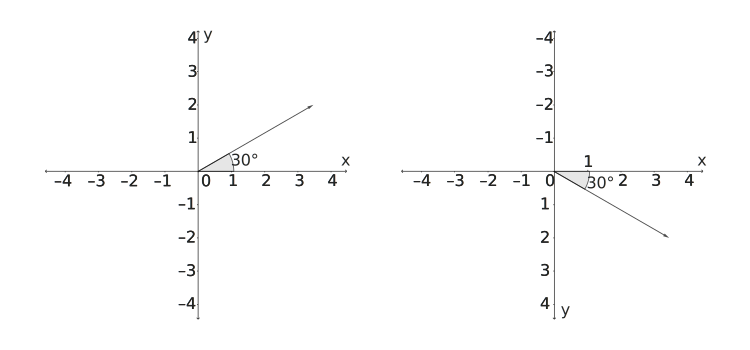
\includegraphics[width=\maxwidth{\textwidth}]{../img/cartesian-systems.pdf}
  \caption[Pravotočivá a levotočivá kartézská soustava souřadnic]{Pravotočivá (vlevo) a levotočivá (vpravo) kartézská soustava souřadnic}
  \label{fig:cartesian-systems}
\end{figure}

Na Obrázku~\ref{fig:cartesian-systems} jsou znázorněny dva typy kartézské soustavy souřadnic -- pravotočivá a levotočivá.
V matematice a geometrii je nejběžnější pravotočivá soustava souřadnic, nicméně \acrshort{svg} používá levotočivou (angl.~left-handed), jak je tomu běžné u počítačové grafiky.
Pro převod úhlu z běžně uvažovaného pravotočivého do levotočivého \acrshort{svg} úhlu slouží právě metoda \texttt{toLeftHandedSystem}.
Ta přijde vhod při rotování vektorů, či celých \acrshort{svg} konstruktů.

Třída \texttt{GlobalIdGenerator} slouží jako generátor identifikátorů a klíčů pro naše objekty.
Zajišťuje, že vždy vrátí unikátní číslo jako nový identifikátor.
Jednoduchá implementace je začít s číslem 0 a každé další zvětšit o 1.
Tato třída je singleton, jeden z objektově orientovaných designových vzorů uvedený Gammou a kol. (také známých jako \enquote{Gang of Four})~\cite[s.~144]{gamma_designpatterns_1995}.
Tím může existovat nejvýše jedna její instance v běžícím systému.

Třída \texttt{SvgPathStringBuilder} konstruuje \acrshort{svg} path data atribut \cite[\S~9.3]{brinza_svg_2018}.
Obsahuje mnoho dalších metod.
Kromě těch, které lze vidět na Obrázku~\ref{fig:utils-class-diagram}, například pro každý příkaz lze pozice (location) specifikovat i relativně k předchozí pozici (místo absolutně).
Třída odpovídá vzoru builder~\cite[s.~110]{gamma_designpatterns_1995}.
Užívání této třídy odpovídá vypisování \enquote{příkazů} pro path data atribut.
Užitečnost této třídy spočívá v přehlednosti -- je lepší používat její metody s deskriptivním názvem místo path data příkazů, které mají formu jednoho písmene a argumentů.

\section{Scénáře}

Případy užití definují funkcionalitu systému a reprezentují se diagramem případů užití (use case diagram).
Každý případ užití popisuje jeden způsob, jak lze systém použít.
Uživatelé systému (lidé, stroje, nebo jiné systémy) jsou v diagramu reprezentováni tzv. herci (actors).
Model tak popisuje způsoby, kterými lze systém použít jeho okolím a jaké služby systém nabízí.~\cite[s.~65]{overgaard_usecases_2005}

Případy užití nebudeme popisovat všechny, kvůli stručnosti.
Dále některé případy užití jsou si velmi podobné, například export do \acrshort{svg} je téměř stejný jako export do \acrshort{png}, akorát se u \acrshort{svg} nevolí barva pozadí.
Zvolíme tedy případy užití, které nějak modelové nebo zásadní.

\begin{figure}[!htb]
  \centering
  \includegraphics[width=\maxwidth{0.7\textwidth}]{../img/diagrams/use-case-diagram.pdf}
  \caption{Diagram případů užití}
  \label{fig:use-case-diagram}
\end{figure}

\newcommand{\ucsub}[1]{\textbf{#1}}
\newcommand{\uc}[1]{\subsection*{#1}}
\def\ucstart{\ucsub{Počáteční stav}\\\indent}
\def\ucnormal{\ucsub{Běžný průběh}}
\def\ucerrors{\ucsub{Možné chyby}}
\def\ucend{\ucsub{Stav systému po dokončení}\\\indent}

\uc{Přidání entitního typu do \acrshort{er} diagramu}
\ucstart{}
V systému je rozdělaný projekt.
\acrshort{er} diagram lze editovat.

\ucnormal{}
\begin{enumerate}
  \item Uživatel přetáhne myší konstrukt \enquote{entitní typ} z panelu konstruktů do \acrshort{er} diagramu.
  \item V diagramu je vytvořen nový entitní typ s výchozím názvem.
  \item Uživatel zvolí právě vytvořený entitní typ myší.
  \item V panelu \enquote{Control Panel} upraví vlastnost entitního typu \enquote{label}.
  \item Název entitního typu se změní na uživatelem definovaný.
\end{enumerate}

\ucend{}
V diagramu je nový entitní typ, který má uživatelem definovaný název.
Změna se projeví i ve schematické kategorii, respektive ve \acrshort{vsk}.

\uc{Přidání atributu k entitnímu typu v \acrshort{er} diagramu}
\ucstart{}
V \acrshort{er} diagramu je entitní typ. Diagram lze editovat.

\ucnormal{}
\begin{enumerate}
  \item Uživatel pravým tlačítkem myši klikne na entitní typ.
  \item Otevře se kontextové menu.
  \item Uživatel zvolí položku \enquote{Add attribute type}.
  \item Do \acrshort{er} diagramu je přidán nový atribut, který je spojen s entitním typem.
  \item Uživatel zvolí právě vytvořený atribut myší.
  \item V ovládacím panelu upraví vlastnost \enquote{label}.
  \item Název atributu je nastaven na právě uživatelem definovaný.
  \item Uživatel případně zvolí spojení mezi entitním typem a atributem myší.
  \item V ovládacím panelu zvolí kardinalitu ze čtyř předdefinovaných možností.
  \item Tato kardinalita je pro spojení nastavena.
\end{enumerate}

\ucend{}
V modelu systému je uložen nový atribut entitního typu, který má daný název a kardinalitu.
Změna se projeví i ve schematické kategorii, resp.~ve \acrshort{vsk}.

\uc{Přidání spojení mezi dva \acrshort{er} elementy diagramu}
\ucstart{}
V \acrshort{er} diagramu dva existující elementy.

\ucnormal{}
\begin{enumerate}
  \item Uživatel zvolí první element levým tlačítkem myši.
  \item Uživatel klikne na druhý element pravým tlačítkem myši.
  \item Zobrazí se kontextové menu.
  \item Uživatel zvolí položku \enquote{New connection}.
  \item Mezi elementy se vloží spojení.
\end{enumerate}

\ucerrors{}
\begin{itemize}
  \item Elementy mohou být nekompatibilní -- např. dva vztahové typy, dva entitní typy.
\end{itemize}

\ucend{}
V modelu i v zobrazeném diagramu bude mezi elementy nové spojení.
\uc{Přidání vztahového typu do \acrshort{er} diagramu}
\ucstart{}
V diagramu je entitní typ nebo více entitních typů, které se budou účastnit vztahového typu.
Případně je lze vytvořit i v průběhu toho případu užití.
Změna se projeví i ve schematické kategorii, resp.~ve \acrshort{vsk}.

\ucnormal{}
\begin{enumerate}
  \item Uživatel z panelu s konstrukty myší přetáhne vztahový typ do \acrshort{er} diagramu.
  \item V \acrshort{er} diagramu se objeví nový vztahový typ.
  \item Uživatel v ovládacím panelu změní název vztahového typu.
  \item Uživatel spojí entitní typ se vztahovým typem podle už popsaného případu užití spojování elementů. Tím přidá účastníka vztahového typu.
  \item To zopakuje s dalšími účastníky (ne nutně jinými).
\end{enumerate}

\ucend{}
V systému je nyní nový vztahový typ s účastníky. To se projeví i ve schematické kategorii, resp.~\acrshort{vsk}.

\uc{Export libovolného diagramu do \acrshort{png}}
\ucstart{}
V systému je rozdělaný projekt.

\ucnormal{}
\begin{enumerate}
  \item Uživatel zvolí položku \menu{File > Export as > PNG} v hlavním menu aplikace.
  \item Otevře se dialog s možnostmi exportu s výběrem diagramu k exportu. Výchozí zvolený diagram bude ten, ve kterém naposledy uživatel pracoval.
  \item V dialogu dále uživatel zvolí, jestli chce do \acrshort{png} souboru zahrnout i serializovanou verzi projektu, aby šel později \acrshort{png} soubor otevřít v aplikaci.
  \item Uživatel v dialogu dále zvolí, jestli má \acrshort{png} mít barvu pozadí, případně jakou. Výchozí nastavení je \acrshort{png} bez pozadí, tedy transparentní.
  \item Uživatel potvrdí dialog.
  \item V prohlížeči uživatele se \enquote{stáhne} exportovaný \acrshort{png} soubor, který má název odpovídající názvu projektu.
\end{enumerate}

\ucerrors{}
\begin{itemize}
  \item V zařízení uživatele není dostatek persistentní paměti na uložení obrázku. O zachycení a obstarání této chyby se stará webový prohlížeč uživatele.
  \item Uživatel zruší dialog místo potvrzení. V takovém případě se nic dalšího nestane (nedojde k exportu).
\end{itemize}

\ucend{}
V uživatelské složce nastavené ve webovém prohlížeči na uložení stahovaných souborů bude uložen \acrshort{png} soubor s rasterizovaným diagramem.

  \chapter{Implementace}\label{chapter:implementace}

V této kapitole popíšeme postup implementace aplikace na kresbu diagramů \acrfull{er}, \acrfull{vsk} a syrových schematických kategorií.

\section{Použité technologie}

K vývoji jsme použili framework React~\cite{react_2023}.
React zjednodušuje tvorbu webových uživatelských rozhraní a celých webových aplikací tím, že umožňuje vytvářet celé komponenty a skládat z nich další.

Programovací jazyk jsme zvolili TypeScript~\cite{microsoft_typescriptjavascript_2023}, který k JavaScriptu přidává statické typování.
Výsledkem kompilace je JavaScript, který lze interpretovat prohlížečem.

Pro správu globálního stavu aplikace jsme použili knihovnu Zustand~\cite{daishikato_zustand_2023}.
V React totiž každá komponenta má svůj stav, který předává jako vlastnosti svým dětem.
Úprava stavu musí být uskutečněna dětmi pomocí události, kterou odebírá rodič.
V našem případě, kdy v jednom diagramu bude mnoho volných komponent (konstruktů), které mezi sebou potřebují komunikovat tento přístup není vhodný.
Přestože v React existují způsoby pro sdílení globálního stavu (React Context), jejich metoda sdílení stavu pro naši aplikaci není vhodná.
Zustand umožňuje vytvořit React Hook, pomocí kterého můžeme v libovolné komponentě číst i upravovat jeden globální stav.

Knihovna Zundo~\cite{kornoelje_zundo_2023} umožňuje globální stav vracet o stav zpět a dopředu (undo/redo).
Ovšem zachytává i nepatrné změny a tak se sledování stavů musí vhodně vypínat a zapínat.

Dále využijeme knihovnu Immer~\cite{michelweststrate_immer_2023}, která umožňuje v React stav mutovat.
Při použití Reactu by se totiž stav přímo mutovat neměl, protože by nebyla zaregistrována jeho změna, React by na ni nemohl náležitě zareagovat a došlo by k nekonzistenci.
React změnu stavu detekuje referenčním (ne hlubokým) porovnáním předchozího a nového stavu komponenty.
Při každé změně stavu se proto běžně musí vytvořit nový objekt.
Pokud je objekt hluboce zanořený, je tvorba nového objektu velmi explicitní a zdlouhavá na programování.
React by se správně měl používat bez zanořených stavů, takže každá komponenta se stará o svůj minimální stav.
Protože však používáme jeden složitý globální stav, Immer je vhodná pomoc.
Immer udělá většinu práce za nás tím, že vytvoří tzv. draft (pracovní verze) stavu a sleduje změny, které na něm program dělá.
Pomocí těchto změn pak vytvoří novou instanci stavu.
Porovnání práce se stavem bez a s knihovnou Immer lze vidět v Kódu~\ref{code:immer}.

Další důležitou použitou knihovnou je class-transformer~\cite{attilaolah_classtransformer_2023}.
V JavaScriptu, resp. v TypeScriptu existují dva druhy objektů -- \emph{plain} a \emph{class} objekt.
Při serializaci class objektů do JSON~\cite{tc39group_jsondata_2017} a zpět ztrácí objekt své metody, metody předků a další informace o třídě, z které byla zkonstruována jeho instance.
Knihovna class-transformer umožňuje mezi těmito typy objektů převádět a my tak můžeme používat instanční metody na objektech deserializovaných z JSON.
Knihovna nefunguje perfektně pro všechny druhy datových složek, a pokládá na třídy další určité restrikce.

Pro zjednodušení práce s CSS styly používáme knihovnu Tailwind CSS~\cite{tailwindlabs_tailwindcss_2020}.
Tailwind CSS proráží metodu nastavování stylů pomocí tzv. utilitních tříd.
Velmi dobře se kombinuje s frameworkem React, protože místo psaní stylů do CSS souborů s arbitrárními názvy, Tailwind CSS umožňuje styl komponent upravovat přímo v jejich atributu \texttt{class}.
Například, pokud chceme nastavit okraje ovládacího prvku na 24 pixelů, použijeme třídu \texttt{m-6}, kde \texttt{m} je zkratka ze slova margin (okraj) a \texttt{6} znamená \enquote{šestá úroveň}.
Úrovně různých nastavení mají předdefinované (ale nastavitelné) hodnoty a umožňují konzistentní styl -- délky, barvy i celé kombinace několika vlastností.
Při kompilaci aplikace se ve výsledném balíčku CSS zakomponují z Tailwind CSS pouze třídy, které byly v aplikaci opravdu použity.

Pro kompilaci a vytvoření výsledného balíčku statické webové aplikace používáme nástroj Vite (čte se francouzsky, [vít]).
Výstupem této kompilace je ideálně pouze jediný HTML soubor, jediný JavaScript soubor a jediný CSS soubor, které jsou připraveny na nasazení.
Vite totiž přeloží TypeScript do JavaScriptu, najde a propojí všechny importované moduly a spojí vše do jediného souboru.
\mcomment{Stačí pro použité technologie takhle strana? Mám ještě o čem psát, konkrétně třeba knihovny na úpravu datových chunků PNG souborů.}

Stěžejní knihovnou, která poskytuje prvky uživatelského rozhraní, je FlexLayout~\cite{_flexlayout_2023}.
Jedná se o rozhraní s okny, která se dají přesouvat, roztahovat a přepínat záložkami.
Tato knihovna byla zvolena, protože je flexibilní a uživatel si své pracovní prostředí díky jejím prvkům může libovolně upravit.

\begin{lstlisting}[language=JavaScript,float=htb,caption=Použití knihovny Immer,label=code:immer]
// tvorba stavu v React
const [state, setState] = useState({
  person: {
    name: "Name",
    age: 30,
    inventory: {
      description: "Description",
      productIds: [1,2,3]
    }
  }
});

// aktualizace stavu bez knihovny Immer
setState(prevState => ({
  ...prevState,
  person: {
    ...prevState.person,
    inventory: {
      ...prevState.person.inventory,
      productIds: [...prevState.person.inventory.productIds, 4]
    }
  }
}))

// aktualizace stavu s knihovnou Immer
setState(produce(draft => {
  draft.person.inventory.productIds.push(4)
}))
\end{lstlisting}

\section{Uživatelská dokumentace}
Pro potřeby uživatele popíšeme uživatelské rozhraní aplikace, jehož ukázku lze vidět na Obrázku~\ref{fig:user-interface}.

\begin{figure}[!htb]
 \centering 
 \includegraphics[width=\maxwidth{\textwidth}]{../img/app/user-interface.png}
 \caption{Ukázka uživatelského rozhraní aplikace}
 \label{fig:user-interface}
\end{figure}

V horní liště aplikace se nachází menu.
Tlačítko File obsahuje možnosti pro vytvoření nového projektu a pro export.
Tlačítko Edit obsahuje možnosti Undo a Redo.
Následuje přepínač \enquote{Sync Pan \& Zoom}, který zamkne synchronizaci pozice pláten.
Přetažení a přiblížení v jednom plátně tak způsobí totožný přesun a přiblížení ve všech ostatních plátnech.
Poslední položkou horní lišty je editovatelné textové pole s názvem diagramu.
Tento název se odráží v názvu souboru při exportu diagramu.

Rozhraní aplikace se skládá z oken, která obsahují záložky s různým obsahem.
Záložky lze přesouvat mezi okny a přetahovat přes jiné záložky myší, čímž může být vytvořeno nové okno.
Při přetahování je uživateli intuitivně vizuálně znázorněno, která z akcí se stane po puštění záložky.
Okna lze zvětšovat a zmenšovat přetažením jejich krajů.
Pokud v nějakém okně nezůstane ani jedna záložka, okno zanikne.
\mcomment{K uživatelské dokumentaci ještě něco dodám, až budu mít dodělanou aplikaci.}

Právě aktivní okno je zvýrazněno světle modrou barvou.
Tato informace říká, kterým plátnem se bude řídit synchronizace pozic, a který diagram bude výchozí při exportování.

Záložka s názvem Control Panel obsahuje ovládací panel, ve kterém lze upravovat hodnoty jednotlivých vlastností elementů diagramu.
Lze ho pozorovat na Obrázku~\ref{fig:control-panel}, kde je zvoleno spojení, jehož kardinalitu a kotvy lze přenastavit v ovládacím panelu.

Záložka s popiskem Drag and Drop, která je také vidět na Obrázku~\ref{fig:control-panel} v levém dolním rohu, obsahuje konstrukty, které lze podržet a přesunout myší do plátna, čímž dojde k vytvoření daného konstruktu v daném plátně.

Význam záložek s popisky \acrshort{er} Diagram, Schemcat Diagram a Schemcat Visualization je zřejmý -- obsahují popořadě plátna pro \acrshort{er} diagram, schematickou kategorii a vizualizaci schematické kategorie.

\begin{figure}[!htb]
 \centering 
 \includegraphics[width=\maxwidth{\textwidth}]{../img/app/control-panel.png}
 \caption{Ukázka ovládacího panelu}
 \label{fig:control-panel}
\end{figure}

\section{Technická dokumentace}

Zdrojový kód aplikace je k dispozici elektronické příloze, viz Příloha~\ref{appendix:electronic}.
Popíšeme zde některé důležité složky se zdrojovým kódem aplikace.

\begin{description}
  \item[\directory{src/components}] obsahuje React komponenty.
    Podsložky seskupují více podobných komponent.
    Některé z nich uvedeme.
  \item[\directory{src/components/UserControls}] seskupuje komponenty základních uživatelských prvků -- zaškrtávací pole, komponenta pro výběr barvy uživatelem, atd.
  \item[\directory{src/components/Menu}] seskupuje komponenty, které se týkají hlavního menu v horní liště aplikace a kontextového menu.
  \item[\directory{src/components/Dialog}] seskupuje komponenty dialogů pro export a potvrzování akcí.
  \item[\directory{src/hooks}] obsahuje React hooks, včetně důležitého \texttt{useStore.ts}, který obstarává instanci modelu s pomocí knihovny Zustand a jeho editaci pomocí knihovny Immer.
  \item[\directory{src/model}] obsahuje soubory, ve kterých se nacházejí jednotlivé třídy modelu.
  \item[\directory{src/utils}] obsahuje soubory s operacemi, které se týkají transformace textových řetězců, práce s poli, apod.
\end{description}

Vedle některých souborů, např.~\texttt{Array.ts}, sídlí i soubory se stejným názvem, pouze odlišnou příponou, např.~\texttt{Array.test.ts}.
Tyto soubory obsahují unit testy, které ověřují funkcionalitu některých operací.

Vstupním bodem aplikace je soubor \directory{index.html}, který volá jediný skript -- \directory{src/main.tsx}.
Úkolem tohoto skriptu je do \acrshort{dom} stromu připojit framework React a vložit do něj hlavní komponentu aplikace.
Soubor obsahující hlavní komponentu aplikace je \directory{src/App.tsx}.
Tato komponenta se stará o přípravu uživatelského rozhraní za použití komponent z knihovny FlexLayout.
Do nich poté nasazuje vlastní komponenty aplikace.
Některé komponenty blíže popíšeme.

\begin{description}
  \item[ControlPanel] představuje ovládací panel, ve kterém uživatel mění hodnoty vlastností elementů diagramu.
    V modelu je pomocí dekorátorů (funkce jazyku TypeScript) určeno, který ovládací prvek má být použit pro kterou vlastnost třídy daného elementu.
    Tato informace je pak za běhu použita k použití správné komponenty.
    Jde o způsob reflexe, který je v TypeScriptu v době psaní práce experimentální (\texttt{reflect-metadata}).
  \item[AnchorPicker] slouží pro výběr kotvy, tj. bodu, kde má být přichyceno spojení na elementu diagramu.
  \item[Draggable] je obecná komponenta, která očekává děti a umožňuje jejich přetahování uživatelem.
  \item[ErNode] představuje element \acrshort{er} diagramu, tedy buď entitní typ, vztahový typ, nebo atribut.
    Který tvar vykreslí, rozhodne pomocí hodnoty typu \texttt{ErNodeType} z modelu.
  \item[IdentifierFence] je komponenta zodpovědná za vykreslování složených identifikátorů.
    Ty jsou vykresleny jako část obvodu obdélníku s oblými rohy, kterému říkáme \emph{fence} (neboli plot).
    V pracovní verzi se místo toho používaly Beziérovy křivky.
    Výsledek však nebyl dostatečně estetický.
  \item[PannableZoomableSvg] reprezentuje \acrshort{svg} plátno, které lze přesouvat, přibližovat a oddalovat myší.
    Dosahuje toho přepočítáváním \acrshort{svg} atributu \texttt{viewBox}.
\end{description}

Většina souborů obsahuje komentáře a TSDoc~\cite{microsoft_whattsdoc_2023} dokumentaci.

\section{Vývoj}\label{section:development}

K vývoji je potřeba mít nainstalovaný Node JS~\cite{openjsfoundation_nodejs_2023}.
Naše prostředí má Node verze 20.
Po instalaci by měl být k dispozici program \texttt{corepack}, kterým lze aktivovat náš upřednostňovaný správce balíčků \texttt{pnpm}~\cite{pnpm_pnpmfast_2023}.
Spustíme příkaz\footnote{rozsah \texttt{\^{}8} specifikuje verzi použitou v době psaní práce, nejnovější verzi lze nainstalovat tím, že místo tohoto rozsahu použijeme \texttt{latest}}
\begin{verbatim}
corepack prepare --activate pnpm@^8
\end{verbatim}
a poté ve složce \directory{schemcat} se zdrojovým kódem spustíme
\begin{verbatim}
pnpm install
\end{verbatim}
což nainstaluje všechny potřebné závislosti.

Poté lze používat všechny příkazy, které jsme definovali v souboru \texttt{package.json}.
Např.~příkaz
\begin{verbatim}
pnpm run dev
\end{verbatim}
spustí vývojový server, který sleduje změny ve zdrojovém kódu a sám stránku webového prohlížeče aktualizuje, když se kód změní.
To umožňuje rapidní cyklus vývoje a testování změn.

Příkaz
\begin{verbatim}
pnpm run build
\end{verbatim}
sestaví projekt a výsledné soubory připravené k nasazení uloží do složky \texttt{dist}.

\section{Instalace a nasazení}

Kromě zdrojového kódu je v Příloze~\ref{appendix:electronic} také sestavený projekt.
Stačí, aby správce soubory přesunul a nasadil na statický webový server.
Tento statický server však musí při odesílání souborů přes \acrshort{http} přiřazovat korektní \acrshort{mime} hlavičky, jinak není fungování projektu zaručeno.

Uživatel musí mít moderní webový prohlížeč, který podporuje ES6 moduly\footnote{prohlížeče definované v tabulce na této adrese \url{https://caniuse.com/es6-module}}.
Pokud je potřeba přidat podporu starších prohlížečů, je třeba postupovat podle Sekce~\ref{section:development}.
Dále nainstalovat balíček \texttt{@vitejs/plugin-legacy}\footnote{\url{https://www.npmjs.com/package/@vitejs/plugin-legacy}}.
Poté je třeba definovat v souboru \texttt{package.json} položku \texttt{browserslist} s rozsahem webových prohlížečů, které chceme podporovat podle specifikace\footnote{\url{https://browsersl.ist/}}.
Nakonec je nutné projekt sestavit.

Pokud chceme sestavený projekt spustit lokálně a máme nainstalovaný správce balíčků ze Sekce~\ref{section:development}, stačí spustit příkaz
\begin{verbatim}
pnpx http-server .
\end{verbatim}
ve složce se soubory sestaveného projektu.
Na obrazovce se pak vypíší lokální adresy, na kterých běží tento statický server.

  \chapter*{Závěr}
\addcontentsline{toc}{chapter}{Závěr}

Tato práce se zabývala využitím schematické kategorie~\cite{svoboda_categorical_2021} jako prostředkem ke konceptuálnímu modelování s vyšší vyjadřovací schopností, než mají běžné modely, včetně \acrshort{er} a \acrshort{uml}.
Jedná se o čerstvý koncept, který by mohl unifikovat různé databázové systémy a smazat rozdíly mezi konceptuální a logickou vrstvou.
Konceptuální modelování pomocí schematických kategorií je obecnější a má vyšší vyjadřovací schopnost než kterákoli existující řešení, která jsme analyzovali v této práci.

Za účelem přiblížení k realizaci tohoto ambiciózního cíle unifikace konceptuálního modelování byla vyvinuta webová aplikace, která umožňuje konceptuální modelování v \acrshort{er} a automatický převod modelu do schematické kategorie.
Aplikace umožňuje interaktivně prozkoumávat schematickou kategorii a také přibližuje její strukturu pomocí navržené vizualizace schematické kategorie.
Dovolí tak zkušeným databázovým inženýrům a softwarovým analytikům seznámit se se schematickou kategorií s pomocí něčeho, co už znají -- \acrshort{er} modelu.
Aplikace dále umožňuje výzkumníkům, kteří pracují se schematickou kategorií, rychlejší experimentování.

Při implementaci aplikace s pomocí zvolených technologií však došlo k mnoha problémům.
Největším viníkem byla nejspíše volba frameworku React, která se před implementací zdála být vhodným kandidátem pro zrychlení vývoje jednostránkové moderní webové aplikace.
Bohužel se při vývoji ukázalo, že React klade restrikce na model aplikace a dále například neumožňuje jednoduchý tok dat mezi sourozenci ve stromě webového dokumentu.
Jelikož diagramy obsahují skoro výhradně komponenty, které jsou svými sourozenci, bylo obtížné vytvořit algoritmy, které kontrolují validitu diagramů apod.
Dalším způsobeným problémem bylo, že React požaduje, aby všechny instance dat byly immutable.
Úprava diagramu se tak ztížila.

Tyto a další problémy byly částečně vyřešeny knihovnami pro React, které ale také měly své chyby.
Například knihovna Zustand umožnila správu globálního stavu, který je k dispozici všem komponentám v aplikaci.
Nicméně komponenty kvůli tomu musely obsahovat spoustu opakujícího se kódu, který zajistil reagování komponenty na změnu globálního stavu.
React je více vhodný při práci ve větším týmu na dlouholetých projektech, kvůli svému zaměření na izolované komponenty.
Autor práce neměl s frameworkem větší předchozí zkušenost a pro příště by volil jiný způsob implementace webové aplikace při samostatné práci v jednom člověku.
Například by se mohlo jednat o vanilla JavaScript, který umožňuje přímou mutaci modelu.

Zdlouhavým a problémovým procesem byl vývoj algoritmu, který vykresluje složené identifikátory.
Při vývoji se prošlo dvěma odlišnými přístupy -- Beziérovými křivkami a obdélníky s oblými rohy.
U obou přístupů bylo obtížné najít polohu průsečíků křivky identifikátoru se spojeními, které křižuje, a posléze volba pořadí průsečíků pro vykreslení co nejkratší křivky.
Algoritmus funguje stabilně, nicméně je určitě prostor pro jeho vylepšení, co se týče stručnosti a výkonnosti.

Celkově byla aplikace a zvlášť její model vyvinut s možností rozšíření na mysli.
Prostor pro rozšíření funkcionality aplikace spočívá například v přidání dalších známých prostředků k tvorbě konceptuálního modelu (např. \acrshort{uml}), možnosti přímého modelování pomocí schematických kategorií, přidání distanční živé spolupráce, a více validací korektnosti diagramů.


  \include{literatura}

  %%% Obrázky v bakalářské práci
  %%% (pokud jich je malé množství, obvykle není třeba seznam uvádět)
  \listoffigures

  %%% Tabulky v bakalářské práci (opět nemusí být nutné uvádět)
  %%% U matematických prací může být lepší přemístit seznam tabulek na začátek práce.
  \listoftables
\else
  % DRAFT VERZE
  % \title{\NazevPrace}
  % \author{\AutorPrace}
  % \date{Draft \today}

  % \include{titulka}
  \tableofcontents
  \chapter*{Úvod}
\addcontentsline{toc}{chapter}{Úvod}

\todotext{Úvod}

  \chapter{Existující nástroje}

V~této kapitole zanalyzujeme některé existující nástroje pro tvorbu diagramů
a~porovnáme je dle navržených kritérií. Nástroji, které budeme porovnávat jsou
\begin{itemize}
  \item diagrams.net~\cite{diagramsnet21} vhodné pro tvorbu libovolných diagramů,
  \item drawSQL~\cite{drawsql21} určené pro tvorbu relačních schémat,
  \item ERDPlus~\cite{erdplus21} k~vytváření zejména ER diagramů~\cite{Chen76}.
\end{itemize}

Před představením existujících nástrojů určíme srovnávací kritéria, dle kterých
budeme nástroje analyzovat.

\section{Srovnávací kritéria}

Prvním kritériem pro porovnání nástrojů je jejich kategorie, která vypovídá
o~účelu nástroje a~cílové skupině zákazníků. Základní kategorie jsou
\begin{itemize}
  \item konceptuální vrstva -- tyto nástroje jsou většinou určené pro tvorbu ER
  diagramů, případně jiným způsobem modelují vztahy a~atributy entit, na které
  při datovém modelování vymezujeme svůj diskurz,
  \item logická (též technologická) vrstva -- tyto nástroje umožňují tvorbu
  diagramů s~ohledem na typ struktur, v~kterých jsou data uchovávána, např.
  relační databáze,
  \item kresba libovolných diagramů -- nástroje, které nejsou omezeny téměř
  žádným standardem či konvencí a~umožňují kresbu libovolných diagramů,
  \item kresba omezených diagramů -- nástroje, které umožňují kresbu diagramů
  omezených na existující schémata (ER, UML~\cite{uml2017}, \dots).
\end{itemize}

Dalším kritériem je typ úložiště. Nástroje mohou ukládat svá data do paměti
prohlížeče (lokálně pro uživatele), na své servery, nebo používat externí
úložiště uživatele, například Google
Drive\footnote{\url{https://www.google.com/drive/}}. Čím více různých typů
úložiště nástroj podporuje, tím lépe, neboť uživatel může flexibilně zvolit jeho
účelům vyhovující způsob uchovávání dat. Pro interaktivní spolupráci s~týmem je
lepší sdílené úložiště a~pro lokální práci je vhodnější lokální úložiště.

Interaktivní spolupráce je dalším důležitým kritériem. U~velkých projektů je
vývoj modelu urychlen, pokud nástroj spolupráci umožňuje.

Dále budeme porovnávat formát, do kterého nástroj diagram ukládá (pokud
k~uloženému souboru má uživatel přístup). Může se jednat o~serializovaný dokument
do dobře známého standardního formátu, nebo o~vlastní formát, který je často
nakonec také založený na nějakém standardu.

Kromě uložení rozdělané práce do vhodného formátu musí nástroj umožnit export do
formátu, který uživatelé využijí pro své účely. Formáty pro export lze rozdělit
do několika kategorií:
\begin{itemize}
  \item serializovaný formát -- většinou se jedná o~vlastní formát aplikace
a~takový soubor nelze jinou aplikací otevřít, ale lze jej programově zpracovat,
  \item rastrové formáty, např. PNG\footnote{Portable Network Graphics --
  \url{https://www.w3.org/TR/2003/REC-PNG-20031110/}} -- mají nejširší využití
  a~podporu, lze je použít v~dokumentech a~na webových stránkách,
  \item vektorové formáty, např. SVG~\cite{Dirk18} -- nemají tak rozšířenou
  podporu, nicméně jsou vhodnější v~dokumentech po estetické stránce (zvlášť při
  tištění); dále existují vektorové editory, pomocí nichž lze výsledek libovolně
  upravovat bez potřeby souboru ve serializovaném formátu; většina webových
  prohlížečů formát SVG podporuje a~soubor vykreslí; do této kategorie lze
  zařadit i~jiné otevřené strukturované formáty, např. VSDX\footnote{Microsoft
  Visio XML formát založený na ISO 29500 --
  \url{https://interoperability.blob.core.windows.net/files/MS-VSDX/\%5bMS-VSDX\%5d.pdf}},
  \item zjednodušený export -- některé nástroje šetří práci uživatele tím, že
  diagram rovnou exportují do HTML\footnote{HyperText Markup Language --
  \url{https://w3.org/TR/2021/SPSD-html52-20210128/}}, PDF\footnote{Portable
  Document Format, ISO 32000 -- \url{https://iso.org/standard/75839.html}}
  a~podobných finálních formátů pro okamžitou aplikaci, přestože uživatel může
  zvolit jiný formát a~finální vytvořit sám,
  \item schématické formáty, např. SQL\footnote{Structured Query Language --
  \url{https://iso.org/standard/63555.html}} -- téměř výhradně u~nástrojů
  lo\-gic\-ké vrst\-vy; umožňují rovnou vytvářet schémata pro databáze.
\end{itemize}

Stejně jako u~typu úložiště, čím více různých formátů exportu nástroj podporuje,
tím lépe, neboť nástroj je flexibilní.

Posledním, neméně důležitým kritériem, je způsob komercializace. Většina volně
dostupných nástrojů je nějakým způsobem zpoplatněna, ať už se jedná
o~jednorázový nebo pravidelný poplatek. Nejčastějším komerčním modelem je verze
zdarma s~omezenými funkcemi a~dále několik placených plánů různé úrovně
s~odemčenými pokročilými funkcemi. U~tohoto modelu je důležité vyrovnat funkce
tak, aby byl nástroj použitelný i~v~bezplatné verzi, a~aby byly placené funkce
atraktivní pro uživatele. Při srovnávání budeme věnovat pozornost i~tomu, jestli
jsou placené funkce esenciální.

\section{diagrams.net}
\label{section:digramsnet}

Srovnávací kritéria:
\begin{itemize}
  \item kategorie -- kresba libovolných diagramů,
  \item typ úložiště -- lokální, externí, prohlížeč,
  \item export -- serializovaný, rastrový, vektorový, zjednodušený,
  \item interaktivní spolupráce -- částečně podporována (pomocí externích úložišť),
  \item komercializace -- veškeré funkce jsou zdarma a~není potřeba uživatelský
  účet; z~jiného pohledu lze počítat cenu externích úložišť, ale ta jsou
  volitelná.
\end{itemize}

Nástroj diagrams.net~\cite{diagramsnet21}, dříve draw.io, je obecný open-source
kreslící nástroj (který však nepřijímá změny od externích vývojářů) vydaný
s~licencí Apache License
2.0\footnote{\url{https://www.apache.org/licenses/LICENSE-2.0}}, dostupný jako
webová aplikace\footnote{na adrese \url{https://app.diagrams.net}} nebo jako
desktopová aplikace. Desktopová verze aplikace je sestavena stejným způsobem
jako webová, pouze je zabalena pomocí platformy Electron~\cite{electron21}  do
okna Chromium. Je vyvinut v~běžných we\-bo\-vých tech\-no\-lo\-gi\-ích
(Java\-Script\footnote{Standardizován jako ECMAScript, ISO 16262 --
\url{https://iso.org/standard/55755.html}}, CSS\footnote{Cascading Style Sheets --
\url{https://www.w3.org/TR/css}}, HTML).

Diagramy lze uložit do serializovaného XML\footnote{Extensible Markup Language
-- \url{https://www.w3.org/TR/xml/}} formátu .drawio. V~tomto formátu je pro
každý diagram XML element \texttt{diagram}, ve kterém se nachází data zakódována
do Base64\footnote{RFC 2045 \S6.8 --
\url{https://datatracker.ietf.org/doc/html/rfc2045\#section-6.8}}. Tato data
jsou komprimována pomocí zlib\footnote{\url{https://zlib.net}} a~obsahují další
XML dokument (URL-encoded\footnote{RFC 3986 \S2.1 --
\url{https://datatracker.ietf.org/doc/html/rfc3986\#section-2.1}}, tj.
zakódovaný), tentokrát již serializaci vlastního diagramu. Formát tak není bez
dekomprese čitelný člověkem. Výhodou je, že lze uložit více diagramů do jednoho
souboru a~každý pojmenovat. Rozhraní k~tomu určené je identické s~listy souboru
tabulkových procesorů, jako Microsoft Excel\footnote{\url{https://aka.ms/excel}}
a~Google Sheets\footnote{\url{https://sheets.google.com}}.

Soubor s~diagramy lze také uložit do formátu SVG, který je navíc otevřený
a~podporují ho jiné nástroje. Uživatel má při exportu k~dispozici možnost
\textit{Include a~copy of my diagram}, která do SVG souboru zahrne již zmíněný
Base64 řetězec, ve kterém je diagram serializovaný. Ve výsledku to znamená, že
takto exportované SVG soubory umí diagrams.net i~otevřít a~práce na nich může
plnohodnotně pokračovat. Toto řešení se nám líbí, protože se jedná o~schování
vlastního formátu do SVG, který je nejvhodnějším pro přechovávání a~zobrazování
diagramů.

Dalšími možnostmi exportu a~ukládání jsou
\begin{itemize}
  \item rastrové soubory PNG, JPEG\footnote{Joint Photographic Experts Group,
  ISO 19566 -- \url{https://iso.org/standard/65348.html}},
  \item soubor PDF, do kterého je ve vektorovém formátu diagram vložen,
  \item soubor HTML, do kterého lze podobně jako v~SVG data diagramu uložit
v~serializované formě, případně pouze vložit veřejný odkaz URL na diagram (pokud
je použito odpovídající úložiště); v~tomto souboru je pak zahrnut JavaScript od
diagrams.net, který diagram vykreslí,
  \item otevřený formát VSDX, původně vyvinutý pro Microsoft Visio.
\end{itemize}

Ze stejných souborů lze diagramy také importovat, ovšem editovat je lze jen
pokud je v~nich zahrnut formát drawio, čehož je dosaženo u~některých formátů
popsaných výše.

Jako úložiště si lze vybrat Google Drive,
OneDrive\footnote{\url{https://aka.ms/onedrive}},
Dropbox\footnote{\url{https://dropbox.com}},
GitHub\footnote{\url{https://github.com}},
GitLab\footnote{\url{https://gitlab.com}}, paměť prohlížeče a~místní úložiště
(disk uživatele). Soubor lze ze stejných úložišť i~otevřít a~importovat, navíc
k~tomu i~z~libovolné dostupné URL.

Interaktivní spolupráce je umožněna pouze pokud soubor jako úložiště využívá
takové, ke kterému mají přístup zápisu (popř. pouze čtení) všichni účastnící se
uživatelé (Google Drive, OneDrive, Dropbox, GitHub, GitLab). Tato úložiště je
však nutno manuálně vhodně nastavit (přístup ostatním uživatelům). U~všech
úložišť je rychlost reflektování změn ostatních uživatelů podobná -- vcelku
pomalá, protože aplikace musí změny aktivně kontrolovat a~načítat.

Menu \texttt{File $\rightarrow$ Publish} chybně napovídá, že se jedná o~funkci
interaktivní spolupráce. Ve skutečnosti je uživateli jen zobrazen odkaz na
soubor ve vybraném úložišti (ale pouze pro Google Drive a~OneDrive, jinak je
tato možnost vypnuta). Spolupracující uživatel tak musí tento soubor v~daném
úložišti uložit k~sobě (sdíleně), aby mohla spolupráce začít.

Jako další možnost jsme zvažovali desktopovou aplikaci s~načteným souborem,
který je libovolným externím nástrojem sdílen mezi uživateli. Bohužel, soubor se
nepřenačítá automaticky, ale musí být manuálně synchronizován tlačítkem
\texttt{File $\rightarrow$ Synchronize (Alt+Shift+S)}, které je dostupné pouze
v~desktopové verzi aplikace. Uživatel je při externí změně souboru upozorněn
(avšak ne spolehlivě vždy) červeným nápisem. Algoritmus synchronizace funguje
správně a~tak, jak uživatel očekává.

Nejlepší způsob dosažení interaktivní spolupráce je dle našeho názoru volba
systému pro správu Git\footnote{Systém pro správu verzí Git --
\url{https://git-scm.com}} repozitářů (GitLab nebo GitHub), protože
\begin{enumerate}
  \item tato úložiště jsou dostupná jak z~webové, tak z~desktopové verze
  aplikace,
  \item synchronizace probíhá pomocí systému Git,
  \item díky použití systému Git lze jednoduše spravovat verze a~body v~historii
  při vývoji diagramu.
\end{enumerate} 

K~poslednímu bodu je třeba podotknout, že jiná webová úložiště také podporují
správu verzí, avšak není tak rozvinutá, jako správa systémem k~tomu určeným --
Git. Diagrams.net sám o~sobě správu verzí neobsahuje, jen obvyklé ``Undo, Redo''
pro aktuálního uživatele. Úpravy ostatních uživatelů nelze vracet postupně, lze
se pouze vrátit za bod synchronizace.

Uživateli jsou v~levém postranním panelu k~dispozici standardní tvary ER
diagramů, UML diagramů~\cite{uml2017}, flowchart diagramů a~další základní tvary
pro kresbu diagramů. Tvary lze libovolně kombinovat a~spojovat podržením levého
tlačítka a~tažením myší z~a~do kotev na krajích objektů. Každý objekt
a~spojovací čára má vlastnosti, které lze upravovat v~pravém postranním panelu.
Upravovat lze přímo i~vlastnosti formátu SVG.

Uživatelské rozhraní, které je vidět na obrázku \ref{fig:diagrams.net}, je velmi
podobné kancelářským aplikacím Google. Je tak přívětivé pro nové uživatele,
kteří již s~aplikacemi Google dříve pracovali.

Jako výhody určujeme
\begin{itemize}
  \item univerzálnost a~flexibilita -- nástroj lze použít pro tvorbu jakýchkoli
  diagramů,
  \item množství podporovaných formátů -- export pokrývá téměř všechny možné
  účely,
  \item cena -- všechny funkce jsou zdarma,
  \item více diagramů v~jednom souboru
\end{itemize}
a~nevýhodami jsou
\begin{itemize}
  \item chybějící možnost pro export do (jednoduše) strojově zpracovatelného
  formátu, nelze tak bez lidské práce diagram převést do logické vrstvy (to je
  zapříčiněno obecností nástroje, jeho účelem je kresba, ne abstrakce),
  \item pomalé zobrazování změn při interaktivní spolupráci, zároveň není
  zpočátku jasné, jak spolupráce dosáhnout.
\end{itemize}

Výhodou i~nevýhodou může být nutnost použití externího úložiště. Pro velké
společnosti se může jednat o~bezpečnostní opatření, protože diagrams.net
k~diagramům nemá přístup. Pro malé týmy se může jednat o~nevýhodu, protože je
potřeba účet na externím webu, nebo jiný způsob sdílení a~správa tohoto
úložiště.

\begin{figure}
  \centering
  \includegraphics[width=\textwidth]{../img/diagrams.net.png}
  \caption{Tvorba ER diagramu v~aplikaci diagrams.net}
  \label{fig:diagrams.net}
\end{figure}

\section{drawSQL}

Srovnávací kritéria:
\begin{itemize}
  \item kategorie -- logická vrstva,
  \item typ úložiště -- online, poskytované autory produktu
  \item export -- schématický (obecný SQL i~platformě specifické formáty),
  rastrový PNG, serializovaný (JSON~\cite{json2017}, v~době psaní práce se
  chystá)
  \item interaktivní spolupráce -- pouze v~placené verzi,
  \item komercializace -- omezená verze navždy zdarma, různé měsíčně placené
  plány.
\end{itemize}

Nástroj drawSQL~\cite{drawsql21} je modelovací nástroj pro tvorbu relačních
schémat. Aplikace je dostupná ve webovém prohlížeči\footnote{na adrese
\url{https://drawsql.app}}. Je vyvinuta ve standardních webových technologiích
a~používá framework Vue.js. Plán zdarma umožňuje tvorbu veřejně přístupných
diagramů, které mohou mít maximálně 15 tabulek (entit). Měsíčně placené plány
umožňují vytvářet neveřejné diagramy, více (až neomezeně mnoho) tabulek
v~diagramu, více uživatelů, kteří mohou na diagramu spolupracovat, a~přístup
k~verzovacím nástrojům. K~vyzkoušení i~používání nástroje je potřeba uživatelský
účet.

Hlavní funkcí drawSQL je export schématu do SQL. Proto si uživatel při vytváření
diagramu zvolí cílovou databázi, pro kterou schéma tvoří. Výsledné SQL tak bude
mít tvar, se kterou cílová databáze umí pracovat. Podporovanými databázemi jsou
MySQL\footnote{\url{https://mysql.com}},
PostgreSQL\footnote{\url{https://postgresql.org}} a~SQL
Server\footnote{Microsoft SQL Server -- \url{https://aka.ms/sqlserver}}.

Rozhraní, které je vidět na obrázku \ref{fig:drawsql}, obsahuje diagram
a~postranní panel. V~postranním panelu lze vytvářet jednotlivé tabulky,
definovat jejich sloupce a~vlastnosti jednotlivých sloupců -- typ sloupce,
nullability\footnote{\emph{nullability} je příznak, který určuje, zda lze sloupec
v~řádku nastavit na hodnotu \texttt{NULL}}, zda se jedná o~primární klíč, unikátní klíč
nebo index. Tyto změny se v~reálném čase reflektují v~diagramu, ve kterém může
uživatel jednotlivé sloupce spojovat, čímž vytváří cizí klíče. Pozici těchto
lomených čar lze upravovat pouze posunutím tabulky v~diagramu. Pokud je cizích
klíčů víc, začne být diagram velmi nepřehledný.

Diagram lze importovat ze souboru SQL stisknutím \texttt{File $\rightarrow$
Import}. Stisknutím tlačítka \texttt{File $\rightarrow$ Export} se otevře
nabídka Export, ve které může uživatel diagram exportovat do SQL své předem
zvolené databáze, nebo do rastrového obrázku ve formátu PNG. Vývojáři aplikace
plánují implementovat také export diagramu pomocí serializace do formátu JSON.
V~nabídce Export je navíc možnost nechat si vygenerovat platformně specifický
kód jako například migrační třídy pro Laravel\footnote{Framework pro PHP --
\url{https://laravel.com}}, definice modelů pro Laravel a~migrační schémata pro
AdonisJS\footnote{Framework pro Node.js -- \url{https://adonisjs.com}}.

Interaktivní spolupráce je k~dispozici pouze v~placené verzi. Dle našeho názoru
je interaktivní spolupráce hlavní funkcí tohoto nástroje oproti konkurenčním
relačním modelovacím nástrojům. Některá integrovaná vývojová prostředí (např.
Visual Studio\footnote{Vývojové prostředí Microsoft Visual Studio --
\url{https://visualstudio.microsoft.com}}) obsahují nástroj pro relační
modelování i~generování databázového schématu. Hlavním omezením těchto nástrojů
je však absence interaktivní spolupráce, jedná se spíše o~spolupráci iterací.
Proto považujeme určení interaktivní spolupráce za placenou funkci za negativní
rozhodnutí pro využitelnost nástroje v~relaci s~konkurencí.

Web drawSQL také zveřejňuje šablony modelů\footnote{na adrese
\url{https://drawsql.app/templates}} (jedná se spíše o~příklady). Šablony jsou
většinou potenciální modely známých produktů (např.
WordPress\footnote{\url{https://wordpress.com}}) a~tvoří je autoři drawSQL.
Tuto funkci považujeme za výhodu, protože společnosti a~individuální vývojáři se
mohou inspirovat existujícími a~ověřenými řešeními, případně nezačínat se svým
modelem od nuly.

Závěrem určíme výhody drawSQL:
\begin{itemize}
  \item příjemné uživatelské rozhraní (viz obrázek \ref{fig:drawsql}),
  \item možnost určení typu relace, o~sémantiku se aplikace stará sama
  (one-to-one, one-to-many, many-to-many),
  \item několik platformě specifických generátorů modelu,
  \item šablony a~příklady existujících modelů
\end{itemize}
a~nevýhody:
\begin{itemize}
  \item nelze upravit ani přesunout lomené čáry spojující cizí klíče, což
  způsobuje chaos pokud je v~diagramu větší množství entit,
  \item interaktivní spolupráce pouze v~placeném plánu,
  \item správa verzí pouze v~placeném plánu,
  \item k~vyzkoušení nástroje je potřeba uživatelský účet,
  \item podporuje pouze relační databáze.
\end{itemize}

\begin{figure}
  \centering
  \includegraphics[width=\textwidth]{../img/drawsql.png}
  \caption{Tvorba diagramu v~drawSQL}
  \label{fig:drawsql}
\end{figure}

\section{ERDPlus}
\begin{itemize}
  \item kategorie -- logická vrstva,
  \item typ úložiště -- online, poskytované autory produktu
  \item export -- rastrový PNG,
  \item interaktivní spolupráce -- není,
  \item komercializace -- zdarma.
\end{itemize}

Nástroj ERDPlus~\cite{erdplus21} je modelovací nástroj pro tvorbu ER diagramů,
relačních schémat a~hvězdicových schémat. Aplikace je dostupná ve webovém
prohlížeči\footnote{na adrese \url{https://erdplus.com}}. Její uživatelské
rozhraní je tedy vyvinuto ve standardních webových technologiích -- HTML, CSS
a~JavaScript -- a~dále využívá framework React~\cite{react2021} pro tvorbu
rozhraní v~jazyce JavaScript.

ERDPlus lze používat bez založení uživatelského účtu a~vytvořený diagram
exportovat do speciálního formátu erdplus, nicméně uživatel tak přijde o~možnost
využití úložiště diagramů na serveru aplikace. Diagramy (ERDPlus je nazývá
\emph{dokumenty}) lze organizovat do složek a podsložek. Služby ERDPlus včetně
úložiště nejsou žádným způsobem zpoplatněny.

Tvorba ER diagramů je intuitivní s~jednoduchým uživatelským rozhraním, které je
vidět na obrázku \ref{fig:erdplus}. Uživatel má na výběr mezi vytvořením entity,
atributu, relace, spojení mezi těmito objekty a~jednoduchého textového popisku.
V~pravé části rozhraní se nachází panel s~vlastnostmi zvoleného objektu. V~tomto
panelu může uživatel také rychleji tvořit atributy entit a~relací. Při zvolení
relace lze v~panelu zvolit entity, které mají být v~relaci, a~spojení je pak
automaticky vytvořeno. Zároveň lze zvolit jednotlivé multiplicity relace.

Soubor s~diagramem je v~úložišti reprezentován vlastním formátem erdplus. Jedná
se o~textový soubor, jehož obsahem je JSON reprezentace diagramu. Diagram lze
exportovat do rastrového formátu PNG.

Zajímavou funkcí je také převod do relačního schématu. Tato funkce je dostupná
pouze tehdy, když uživatel ER diagram uloží na server ERDPlus. Poté zvolí
možnost \emph{Convert to Relational Schema} a~ERDPlus vytvoří nové relační
schéma. Z~relačních schémat lze podobně vygenerovat SQL.

Vlastnoruční tvorba relačních diagramů probíhá podobně. Uživatel může tvořit
tabulky, přidávat jim sloupce a v~tabulkách volit primární klíče v~postranním
panelu. Pomocí tlačítka \texttt{Connect} lze poté přidat cizí klíč, který
odkazuje do jiné tabulky tažením myši. ERDPlus do tabulky přidá všechny primární
klíče, které cílová tabulka obsahuje, jako nové sloupce. K~vytvoření cizího
klíče, který odkazuje na stejnou tabulku (tzv. rekurzivní klíč) slouží tlačítko
\texttt{Recursive Key} ve vlastnostech tabulky. Hvězdicovým schématům se věnovat
nebudeme, protože jsou mimo rozsah této práce.

Výhody:
\begin{itemize}
  \item převod diagramu z~ER do relačního diagramu,
  \item jednoduchost a intuitivnost procesu kresby diagramu 
\end{itemize}
a nevýhody:
\begin{itemize}
  \item relační diagram bývá nepřehledný, nelze měnit pořadí jednotlivých
  definovaných sloupců v~tabulce,
  \item chybí vektorový export,
  \item diagramy nelze stylizovat.
\end{itemize}

\begin{figure}
  \centering
  \includegraphics[width=\textwidth]{../img/erdplus.png}
  \caption{Tvorba ER diagramu v~ERDplus}
  \label{fig:erdplus}
\end{figure}

\section{nomnoml}

\begin{itemize}
  \item kategorie -- kresba omezených diagramů -- UML,
  \item typ úložiště -- online,,
  \item export -- rastrový PNG, vektorový SVG,
  \item interaktivní spolupráce -- není k~dispozici,
  \item komercializace -- zdarma s~otevřeným zdrojovým kódem.
\end{itemize}

Nástroj nomnoml je modelovací nástroj pro tvorbu UML diagramů dostupný ve
webovém prohlížeči\footnote{na adrese \url{https://nomnoml.com}}. Jeho klíčová
vlastnost je, že místo interakce myší s~webovou aplikací probíhá kresba
deklarativně -- psaním.

Uživatelské rozhraní (viz obrázek \ref{fig:nomnoml}) se skládá z~oblasti pro
textový vstup, nad kterou je zároveň (v~reálném čase) vykreslován výsledný
diagram. V~pravé horní části se nachází několik tlačítek, při kliknutí na
některé z~nich se vždy otevře pravý postranní panel s~odpovídajícími informacemi
a funkcemi. První tlačítko ukazuje rychlý přehled jazyka, ve kterém se má
diagram definovat. Druhé tlačítko odhalí kompletní referenci k~tomuto jazyku.
Dále lze najít tlačítka pro export, sdílení a uložení do místního úložiště
uživatele.

Jazyk diagramů je velmi jednoduchý. Skládá se z~definic entit a jejich relací.
Uživatel může vyjít z~úvodního diagramu, který se ukáže při navštívení hlavní
stránky nástroje. Pro ukázku, definice entity vypadá následovně

\noindent\texttt{[<abstract> Entita|soukromaSlozka; soukromaSlozka2|verejnyAtribut]}.

Svislá čára odděluje kategorie atributů, může jich být neomezené množství.
Entita je definována jako abstraktní, což také ovlivní její výsledný styl
vzhledu v~diagramu.

Dále se v~jazyce definují vztahy mezi entitami následovně
\texttt{[Entita]->[Entita2]}. Různé šipky mají různé významy. Vztah \texttt{->}
je \emph{asociace}, dále \texttt{o->} je \emph{agregace}, apod.

V~jazyce lze také deklarovat direktivy, začínající znakem \texttt{\#}. Těmi lze
upravit vzhled, vytvořit nové styly, a nastavit algoritmy, kterými bude zvoleno
rozložení entit v~diagramu. Algoritmy lze nastavit direktivou \texttt{\#ranker}
a na výběr je ze tří možností: \texttt{network-simplex}, \texttt{tight-tree},
\texttt{longest-path}. Nástroj nomnoml používá k~vykreslování diagramu knihovnu
dagre\footnote{\url{https://github.com/dagrejs/dagre}} pro JavaScript, jejíž
vývoj byl však ukončen. Z~dokumentace této knihovny vyplývá, že možnost
\emph{ranker} mění algoritmus, který vrcholům v~grafu (diagramu) přiřazuje
důležitost, která se pak odráží v~pořadí zobrazení entit. Definitivní význam
této možnosti není z~dokumentace zřejmý, u~nástroje nomnoml lze však pozorovat
změnu v~pořadí a vzdálenostech entit (délce spojovacích čar). Uživatel tak může
vyzkoušet různá rozložení a použít to, které je vizuálně nejpřehlednější.

Diagram lze exportovat do formátu PNG a dále podobně jako v~sekci
\ref{section:digramsnet}, nomnoml také umožňuje export do SVG se zakomponovaným
zdrojovým kódem. Uživatel tak může diagram distribuovat v~tomto formátu a
zároveň tento formát v~nástroji nomnoml i otevřít a plnohodnotně pokračovat
v~práci. Podobně je možné sdílet odkaz přímo na vytvořený diagram ve službě
nomnoml. Ten je vytvořen tak, že do odkazu URL je jako parametr \texttt{source}
zapsán přímo zdrojový kód diagramu. Výsledná adresa URL je tak velice dlouhá,
ale služba nomnoml nemusí diagramy ukládat, stačí jej vykreslit z~dat v~odkazu.
Přestože se nejedná o~opravdové online úložiště, kategorizovali jsme ho tímto
způsobem. Rozdělaný diagram lze také uložit do paměti prohlížeče.

Nástroj nomnoml je tedy inovativní svým přístupem ke kresbě diagramů.
U~složitých diagramů se však nutně ve zdrojovém kódu uživatel ztrácí, protože
nomnoml nenabízí žádné dělení čí kompozici tohoto kódu. S~vizuální reprezentací
grafu nelze přímo (např. myší) pracovat, veškeré rozložení a orientaci diagramu
tak musí uživatel nechat na algoritmu nástroje. Nástroj dále nenabízí ani
možnost pracovat s~několika diagramy najednou. Z~těchto důvodů určujeme produkt
jako vhodný pouze pro jednotlivce a tvorbu méně rozsáhlých UML diagramů.

\begin{figure}
  \centering
  \includegraphics[width=\textwidth]{../img/nomnoml.png}
  \caption{Tvorba UML diagramu v~nomnoml}
  \label{fig:nomnoml}
\end{figure}

\section{Závěr existujících řešení}

Přehled analýzy zmíněných existujících řešení je vidět v~tabulce
\ref{tab:existing-comparison}. % TODO doplnit

\newcommand{\tnote}[1]{\textsuperscript{#1}}
\begin{table}
  \begin{center}
    \begin{tabular}{r|cccc}
      \toprule
      název produktu           & \textbf{diagrams.net}                       & \textbf{drawSQL}                                & \textbf{ERDPlus} & \textbf{nomnoml}\\
      \midrule                 
      kategorie (vrstva)       & libovolné d.                          & logická                                         & konceptuální & omezené d. \\    
      serializovaný ex.     & ano                                         & ne\tnote{\ref{tab:ec:plan}}                     & ano & ano \\               
      rastrový ex.         & ano                                         & ano                                             & ano & ano  \\            
      vektorový ex.        & ano                                         & ne                                              & ne & ano \\              
      schématický ex. & ne                                          & SQL                                             & SQL & ne \\             
      zjednodušený ex.      & HTML, PDF                                   & ano\tnote{\ref{tab:scaffolding}} & ne & ne \\               
      poskytuje úložiště       & ne\tnote{\ref{tab:ec:external-storage}}     & ano                                             & ano & ano\tnote{\ref{tab:ec:urlsharing}} \\            
      paměť prohlížeče & ano                                         & ne                                               & ne & ano \\                
      \midrule[\heavyrulewidth]
      \end{tabular}
  \end{center}
  
  \footnotesize
  \begin{enumerate}[a.,ref=\alph*,noitemsep]
    \item plánovaná funkce \label{tab:ec:plan}
    \item využívá úložiště třetích stran \label{tab:ec:external-storage}
    \item platformně-specifický scaffolding -- automatické generování kódu pro specifické platformy a programovací jazyky \label{tab:scaffolding}
    \item diagram je uložen v~URL, pomocí které lze diagram sdílet \label{tab:ec:urlsharing}
  \end{enumerate}
  
  \caption{Srovnání existujících řešení}
  \label{tab:existing-comparison}
\end{table}
  \chapter{Teoretický rámec}\label{chapter:teorie}

V této kapitole představíme potřebné teoretické koncepty, které bude využívat výsledná aplikace.
Mezi tyto koncepty patří \acrfull{er} model a nově vyvíjený konceptuální model v podobě schematické kategorie~\cite{svoboda_categorical_2021} v rozšířené verzi navržené vedoucím práce.

\section{\acrlong{er}}\label{section:entity-relationship}

Datový model \acrfull{er} poprvé představil Peter Pin-Shan Chen už v roce 1976~\cite{chen_er_1976}.
Od té doby se však \acrshort{er} vyvíjel, jak se potřeby datového modelování rozšiřovaly.
\acrshort{er} není standardizováno, ale jednu moderní verzi představili Atzeni, Ceri, Paraboschi a Torlone~\cite[s.~163-179]{atzeni_database_1999}.
Na jejich \acrshort{er} modelu založíme ten náš, který zde popíšeme.

V Tabulce~\ref{tab:er-constructs} jsou vyobrazeny jednotlivé konstrukty \acrshort{er} modelu.

\begin{table}[htb]
  \centering
  \begin{tabular}{@{}rm{9cm}@{}} \toprule
    Konstrukt             & Vizuální reprezentace                                     \\ \midrule
    Entitní typ           & {\centering\includegraphics{../img/er-model/entity.pdf}}  \\
    Vztahový typ          & \includegraphics{../img/er-model/relationship.pdf}        \\
    Atribut               & \includegraphics{../img/er-model/attribute.pdf}           \\
    Složený atribut       & \includegraphics{../img/er-model/composite-attribute.pdf} \\
    Interní identifikátor & \includegraphics{../img/er-model/identifier.pdf}          \\
    Externí identifikátor & \includegraphics{../img/er-model/external-identifier.pdf} \\
    Zobecnění             & \includegraphics{../img/er-model/generalization.pdf}      \\ \bottomrule
  \end{tabular}
  \caption[Grafická reprezentace konstruktů \acrshort{er} modelu]{Grafická reprezentace konstruktů \acrshort{er} modelu, upraveno a přeloženo~\cite[s.~164, Obr.~5.4]{atzeni_database_1999}}
  \label{tab:er-constructs}
\end{table}

Zde blíže popíšeme jejich sémantiku:
\begin{itemize}
  \item Entitní typ (Entity Type) reprezentuje předpis pro instance entit reálného světa.
        Každý entitní typ má jméno, které je unikátní v daném schématu.
  \item Vztahový typ (Relationship Type) reprezentuje vztah mezi dvěma nebo více (ne nutně různými) entitními typy.
        Každý vztahový typ má jméno.
  \item Atribut (Attribute) reprezentuje vlastnost entitních nebo vztahových typů.
        Každý atribut má jednoznačné jméno.
  \item Složený atribut (Composite Attribute) je atribut, který má sám atributy.
        Zakazujeme však další větvení, tedy atributy složeného atributu už samy nemohou být složené.
        Každý složený atribut má sám jméno, podobně jako jeho vlastní atributy.
  \item \label{def:cardinality}Kardinalita (Cardinality) je dvojice $(a, b) \in \set{\zero, \one}\times \set{\one, \many}$, kde $a$ nazýváme minimální kardinalita (spodní hranice) a $b$ maximální kardinalita (horní hranice).
        Kardinalitu musí mít každý atribut a každý účastník vztahového typu.
        Výchozí kardinalita je \oneone{} a ve schématu se většinou neuvádí.
        Spodní hranice 0 znamená, že účast je volitelná; hranice 1 znamená, že účast je povinná.
        Horní hranice 1 znamená, že účast je nejvýše jedna; hranice~\many{} znamená, že účastí je libovolný počet.
        \begin{itemize}
          \item Hranice kardinalit pro jednotlivé účastníky vztahových typů vyjadřují minimální a resp. maximální počet výskytů jednotlivých instancí účastníků v tomto vztahu.
          \item Hranice kardinalit u atributů vyjadřují minimální a resp. maximální počet hodnot atributu, které se vztahují k dané instanci entity/vztahu.
        \end{itemize}
  \item Identifikátor (Identifier) umožňuje jednoznačně rozlišit (identifikovat) instance entitních typů.
        Pro každý entitní typ je povinný alespoň jeden identifikátor, ale může jich být více.
        Každý identifikátor je tvořen buď
        \begin{itemize}
          \item jedním nebo více atributy daného entitního typu; takový identifikátor nazýváme \emph{interní}, nebo
          \item jedním, nebo více vztahovými typy, jichž se daný entitní typ účastní, a žádným či libovolným množstvím atributů daného entitního typu; takový identifikátor nazýváme \emph{externí}.
        \end{itemize}
  \item Zobecnění (generalization), nebo také ISA hierarchie\footnote{ISA z anglického \enquote{is a}, analogicky ke vztahu \enquote{has a}} (ISA Hierarchy), vyjadřuje vztah podobný dědičnosti v objektově orientovaném programování.
        Jde o vztah mezi entiním typem $E$ zvaným \emph{rodič} a jedním nebo více \emph{dětmi} $E_1, \dots, E_n$.
        Všechny vlastnosti rodiče (atributy, identifikátory, spojené vztahové typy a další ISA hierarchie) jsou i vlastnosti každého z dětí.
        Každá instance dítěte je také instancí rodiče.
\end{itemize}

Entitní typy, které nemají ani jeden interní identifikátor (musí mít tedy externí), nazýváme \emph{slabé} entitní typy (weak entity types).
Pokud mají interní identifikátor, nazýváme je \emph{silné} entitní typy (strong entity types).

Vztahový typ se externí identifikace může účastnit nejvýše od jednoho účastníka.
Jinak řečeno, pokud je vztahový typ součástí slabého identifikátoru nějakého entitního typu, daný vztahový typ už nemůže být součástí slabého identifkátoru jiného entitního typu.
Jeden entitní typ však může mít více externích identifikátorů, který každý zahrnuje daný vztahový typ.
Nicméně, externí identifikace se může řetězit, jako na Obrázku~\ref{fig:er-external-identifier-chain}.
Nesmí ovšem vzniknout orientovaný cyklus, a to ani v kombinaci s ISA hierarchiemi.
Formálněji -- pokud vytvoříme orientovaný graf $G=(V,E)$ takový, že
\begin{itemize}
  \item vrcholy $V$ jsou entitní typy a
  \item hrany $E$ jsou
        \begin{itemize}
          \item pro každý externí identifikátor od identifikovaného entitního typu $a$ k identifikujícímu entitnímu typu $b$ orientovaná hrana $(a, b)$,
          \item pro každou ISA hierarchii pro každý vztah rodič-dítě, kde $a$ je dítě a $b$ je rodič, orientovaná hranu $(a, b)$,
        \end{itemize}
\end{itemize}
pak graf $G$ musí být acyklický.

V \acrshort{er} se nesmí vyskytovat identifikátory, které jsou redundantní.
Pro každé dva identifikátory jednoho entitního typu $I, J$, pokud $J\subset I$, pak $I$ je \emph{redundantní}, protože k identifikaci entitního typu stačí $J$.
Všechny atributy a vztahové typy v $I\setminus J$ nejsou potřeba k identifikaci.
Ukázka redundantního identifikátoru je na Obrázku~\ref{fig:redundant-ids}.

\begin{figure}[!htb]
  \centering
  \includegraphics[width=\maxwidth{\textwidth}]{../img/er-model/redundant-ids.pdf}
  \caption{Ukázka redundantního a neredundantního identifikátoru}
  \label{fig:redundant-ids}
\end{figure}

Entitní typ, který má externí identifikátor, musí být účastněn vztahového typu (jímž je identifikován) s kardinalitou $(\one, \one)$.
Teoreticky by se mohl účsatnit i jinou kardinalitou, ale pro naše účely tyto situace modelovat nebudeme.

\begin{figure}[!htb]
  \centering
  \includegraphics[width=\maxwidth{\textwidth}]{../img/er-model/external-id-chain.pdf}
  \caption{Zřetězení externích identifikátorů}
  \label{fig:er-external-identifier-chain}
\end{figure}

U kardinality poznamenejme, že se v \acrshort{er} modelu často dovoluje použít jako hranice libovolná nezáporná celá čísla, tedy $(a, b)\in \mathbb N_0\times \left(\mathbb N_0 \cup \set{\many}\right)$, tž.~$a\leq b$ (dodefinujeme $\forall a\in\mathbb N_0\colon a < \many$).
Dají se tak vyjádřit přesnější omezení, např. že jeden uživatel může mít maximálně 5 bankovních účtů.
Ovšem námi definované hranice kardinality vyjadřují volitelnost/povinnost pro spodní hranici a jednočetnost/mnohočetnost pro horní hranici.
Pokryjeme jimi z teoretického pohledu a s ohledem na povahu konstruktů v nejrůznějších logických modelech všechny strukturálně odlišné situace, které by mohly nastat.

Dále upozorněme, že místo~\many{} se v \acrshort{er} modelu může použít symbol \texttt{n} nebo \texttt{N} pro vyjádření \enquote{libovolného počtu}.
Důležitá je ale konzistentnost, aby se v jednom modelu nevyskytovaly dva různé symboly, což by mohlo zmást čtenáře.
V této práci budeme používat pouze symbol~\many{}.

\section{Schematická kategorie}\label{section:schemcat}

V této sekci popíšeme mechanismus pro konceptuální modelování s názvem schematická kategorie společně s teorií kategorií, na které je založena.
Nejdříve ale představíme motivaci za uvedením nového způsobu konceptuálního modelování.

\subsection{Motivace}\mcomment{Tady se musím více rozepsat}

Při začátku vývoje databázových systémů bylo popsáno několik databázových modelů dat.
Už v roce 1975 je ANSI rozdělila do tří vrstev~\cite{steeljr._interimreport_1975}.
\begin{itemize}
  \item Konceptuální vrstva popisuje část světa, na kterou vymezujeme svůj diskurz.
  \item Logická vrstva popisuje logickou strukturu dat (např. graf, tabulka, \dots).
  \item Fyzická vrstva popisuje, jak jsou data fyzicky uložena v paměťové jednotce.
\end{itemize}

Přestože databázových modelů bylo navrženo několik, časem se ukázalo, že nejužitečnější je ten relační.
To proto, že data byla často tabulkové povahy.
Pokud výjimečně nebyla takové povahy, musela se relačnímu modelu přizpůsobit.

S příchodem potřeby zpracování velkých dat (Big Data)~\cite{cron_bigdata_2012} se ukázalo, že relační model není dostačující.
Ve velkém množství dat, která spolu nutně nesouvisí, není totiž jednoduché najít tabulkovou strukturu.
V různých situacích jsou tedy vhodné různé databázové systémy.
Dokonce se začalo používat více databázových systémů najednou.
Například pro cache lze použít key/value store, pro data různorodé povahy lze použít dokumentové databáze a pro silně strukturovaná data starší relační databáze.

Naše vize do budoucna je mít jediný databázový systém, který má jediné rozhraní, jediný způsob modelování dat a jediný dotazovací jazyk, ale zároveň není závislý na fyzické vrstvě.
V současných systémech je často tvorba a iterace databázových schémat časově náročná a obtěžující.
Chceme proto sloučit konceptuální a logickou vrstvu a předejít tak problémům a lidskému rozhodování při převodu mezi nimi.
Vznikne tak pouze jedna vrstva, ve které se pracuje unifikovaným, konceptuálním způsobem.

Prvním krokem v této vizi by mohly být schematické kategorie, které uživateli umožní popsat strukturu dat, se kterými chce v databázi pracovat.
Jejich koncept popisují Martin Svoboda, Pavel Čontoš a Irena Holubová~\cite{svoboda_categorical_2021}.

Prostředky \acrshort{er} jsou vhodné ke konceptuálnímu modelování, nicméně mají několik nevýhod.
Některé z nich zde identifikujeme.
\begin{itemize}
  \item V \acrshort{er} lze často modelovat jeden případ mnoha způsoby a není předem jasné, který z nich je nejlepší.
        Schematické kategorie většinu takových rozdílů smažou, zejména rozdíly mezi entitními typy, vztahovými typy a atributy.
        Často totiž tyto rozdíly nejsou důležité.
  \item \acrshort{er} zavádí několik omezení, např.~vztahové typy nemohou mít interní identifikátor a složené atributy se nemohou libovolně větvit.
        Tato omezení vznikají, protože se historicky \acrshort{er} používalo zejména pro konceptuální modelování pro relační databáze.
        Libovolně větvené atributy se těžko převedou do relačního modelu.
\end{itemize}

\acrfull{uml}~\cite{omg_uml_2017} také umožňuje vytvářet konceptuální schémata.
Při vývoji software, zvlášť při práci v týmech, je většinou zvoleno \acrshort{uml} oproti \acrshort{er}.
Je to dáno existencí rozličných nástrojů na vytváření \acrshort{uml} diagramů a nástrojů na automatizaci převodu do logické vrstvy.
Vyjadřovací schopnost \acrshort{uml} je nicméně menší, než u \acrshort{er}.
Postupným vývojem \acrshort{uml} se expresivnost dodává.
Nicméně dosahuje se toho přes konstrukty (např.~stereotypy), u kterých lze poznat, že nesouhlasí s původní myšlenkou \acrshort{uml}.

\subsection{Teorie kategorií}

Nejdříve popíšeme obecný pojem kategorie z teorie kategorií, na níž je schematická kategorie založena.

Kategorie je matematická struktura, která zobecňuje mnoho jiných matematických struktur.
Umožňuje tak mimo jiné studovat vztahy mezi nimi.
Poprvé byla představena Eilenbergem a MacLanem v roce 1945~\cite{eilenberg_generaltheory_1945}.

Kategorie $C=(\mathcal O, \mathcal M, \circ)$ se skládá
z \begin{itemize}
  \item množiny objektů $\mathcal O$,
  \item množiny morfismů $\mathcal M$; každý morfismus $f \in \mathcal M$ má zdrojový objekt $A\in\mathcal O$ (budeme naývat také \emph{doména}), cílový objekt $B\in\mathcal O$ (také \emph{kodoména}), ne nutně různý, a zapisujeme $f: A\to B$ ($f$ je morfismus z $A$ do $B$),
  \item operace skládání $\circ\colon \mathcal M\times\mathcal M \to \mathcal M$; pro každé dva morfismy $f,g\in\mathcal M$, tž. $f\colon A\to B, g\colon B\to C$, musí $g\circ f\in \mathcal M$ (tranzitivita); pro tuto operaci navíc platí vlastnosti
        \begin{itemize}
          \item asociativita -- pro morfismy $f,g,h\in\mathcal M$ takové, že $f\colon A\to B, g\colon B\to C, h\colon C\to D$, platí $h\circ (g \circ f) = (h\circ g)\circ f$,
          \item identitní morfismy -- pro každý morfismus $f\in\mathcal M, f\colon A\to B$ a jeho objekty $A$, resp. $B\in\mathcal O$ existují morfismy $1_A$, resp. $1_B\in\mathcal M$, tž. $f\circ 1_A = f = 1_B\circ f$; morfismy $1_A$, resp. $1_B$ nazýváme \emph{identitní morfismy}.
        \end{itemize}
\end{itemize}

Objekty a morfismy lze definovat i obecněji s použitím tříd místo množin, ale pro naše účely budou stačit množiny.

Jako jednoduchý příklad kategorie uvedeme reálná čísla s neostrou nerovností.
Objekty této kategorie jsou reálná čísla $\mathcal O=\R$.
Pro každá reálná čísla $A,B\in\R$ přidáme morfismus $f\colon A\to B$ právě tehdy, když $A\leq B$.
Pro všechny morfismy $f,g\in\mathcal M$ a objekty $A, B, C\in\mathcal O$ takové, že $f\colon A\to B$ a $g\colon B\to C$ definujme $g\circ f=h$, kde $h\colon A\to C$ a $h\in\mathcal M$.

Kategorie je možné vizuálně reprezentovat orientovaným multigrafem, kde vrcholy jsou objekty a orientované hrany morfismy.
Příklad této vizualizace je na Obrázku~\ref{fig:category-example}.
Jedná se o kategorii se třemi objekty $A, B, C$.
Všimněme si, že každý objekt má svůj identitní morfismus.

\begin{figure}[!htb]
  \shorthandoff{"}
  \centering
  % https://tikzcd.yichuanshen.de/#N4Igdg9gJgpgziAXAbVABwnAlgFyxMJZABgBpiBdUkANwEMAbAVxiRAEEQBfU9TXfIRQBGclVqMWbAELdeIDNjwEio4ePrNWiEAGFu4mFADm8IqABmAJwgBbJGRA4ISURK1sLcyzfuI3zkgATNSaUjrG3iDWdg7UgYgh7uEgxgA6aQDGWFaZAARe1Ax0AEYwDAAK-MpCIFZYxgAWOFExfo4JjgwQEGhEQQDsZBaMcDDixWWV1YJs9U0toZLaIMIA+pw8PrH+8S67IN29RACcw6PjRaXlVUqzOvPNIEseOuuyW9G+wXs-hz19FBnUgjBhjCbXaZ3FQPBpPF4pdb6LgULhAA
  \begin{tikzcd}
    A \arrow[r, "f"] \arrow[rd, "g\circ f"'] \arrow["1_A"', loop, distance=2em, in=215, out=145] & B \arrow[d, "g"] \arrow["1_B"', loop, distance=2em, in=35, out=325] \\
    & C \arrow["1_C"', loop, distance=2em, in=35, out=325]
  \end{tikzcd}
  \caption{Příklad kategorie}%
  \label{fig:category-example}%
  \shorthandon{"}
\end{figure}

\subsection{Schematická kategorie}

Schematická kategorie je mechanismus na popis konceptuálního schématu dat založený na teorii kategorií.
Oproti~\acrshort{er} má schematická kategorie větší vyjadřovací sílu.
Její koncept společně s algoritmem převodu z \acrshort{er} schématu do schematické kategorie uvádí~\cite{svoboda_categorical_2021}.
My však použijeme upravenou definici schematické kategorie navrženou vedoucím práce.

Nejprve zavedeme pomocný pojem \emph{signatura}.
Jedá se o řetězec nad abecedou symbolů $\N$.
Prázdný řetězec značíme $\varepsilon$.
Operaci zřetězení značíme symbolem $\cdot$ tečky.
Příklady signatur: $\varepsilon$, $13$, $13\cdot 7$.

Formálně je schematická kategorie instance kategorie $(\mathcal O, \mathcal M, \circ)$ taková, že
\begin{itemize}
  \item každý objekt této kategorie má strukturu trojice: (identita, název, množina identifikátorů), kde
        \begin{itemize}
          \item identita je libovolný symbol z $\N$, který umožňuje rozlišit a unikátně identifikovat každý objekt; tedy speciálně i pro případ, kdy by všechny ostatní složky měl totožné s jiným objektem,
          \item název reprezentuje textovým řetězcem uživatelské jméno daného objektu, může být i prázdný, pak ho značíme $\bot$,
          \item množina identifikátorů obsahuje identifikátory; každý jednotlivý identifikátor je množina identit a vyjadřuje, čím lze daný objekt konceptuálně identifikovat (podobně jako identifikátory z \acrshort{er}),
        \end{itemize}
  \item každý morfismus má strukturu osmice: (signatura, doména, kodoména, název, kardinalita, duplicity, uspořádání),
        \begin{itemize}
          \item signatura byla již popsána jako pomocný pojem; její účel je umožnit (společně s doménou a kodoménou) rozlišit a unikátně identifikovat každý morfismus v daném schématu; jedná se o řetězec vyjadřující orientovanou cestu, složený ze signatur bázových morfismů (zřetězujeme ve stejném pořadí jako se zapisuje skládání morfismů v kategorii, viz Obrázek~\ref{fig:morphism-signatures}),
          \item doména a kodoména odpovídají zdrojovému a cílovému objektu tohoto morfismu,
          \item směr je buď \zero{} (tam) nebo \one{} (zpět) s výchozí hodnotou \zero{}; hodnota \one{} vyjadřuje, že tento morfismus je pouze inverze k jinému, dodaná pro úplnost modelu,
          \item název je uživatelské jméno tohoto morfismu, může být i prázdné $\bot$,
          \item kardinalita je dvojice (min, max), která odpovídá kardinalitě z \acrshort{er} v Sekci~\ref{def:cardinality},
          \item duplicity a uspořádání jsou booleovské hodnoty (\texttt{true}/\texttt{false}), které konceptuálně modelují, zda jsou pro vztažené instance (modelovány kodoménou), která jsou morfismem spojena k vztahované instanci (modelována doménou), povoleny duplicity, resp. jestli mají být uspořádány; tyto hodnoty mají význam, pouze pokud je horní hranice kardinality tohoto morfismu \many; výchozí hodnota obou složek je proto \texttt{false}.
        \end{itemize}
\end{itemize}

Morfismy schematické kategorie rozdělíme na několik vzájemně disjunktních druhů.
Příklad každého druhu lze pozorovat na Obrázku~\ref{fig:morphism-signatures}.
\begin{itemize}
  \item \emph{Bázové} (base) morfismy jsou ty, které vyjadřují konceptuální spojení dvou objektů ze schématu (tedy odpovídají jednotlivým spojením z ER); jejich signatura je jeden unikátní symbol z abecedy.
  \item \emph{Identitní} (identity) morfismy jsou ty, které vznikly jen kvůli splnění stejnojmenného axiomu z definice kategorie; jejich signatura je $\varepsilon$.
  \item \emph{Odvozené} (derived) morfismy jsou ty, které vznikly kvůli tranzitivitě (tedy aby byly morfismy uzavřené na operaci skládání); jejich signatura je opravdová cesta -- zřetězené signatury morfismů, ze kterých byl tento morfismus vytvořen.
\end{itemize}

Ve schematické kategorii bez újmy na vyjadřovací schopnosti zakážeme bázové smyčky (tj. bázový morfismus, jehož doména a kodoména je totožná).
Pokud chceme vyjádřit rekurzivní vztah, můžeme bázovou smyčku nahradit objektem, který tento vztah reprezentuje.
Navíc dodáme dva bázové morfismy, které spojí objekt vztahu s objektem, jehož se vztah týká.

Operaci skládání morfismů $\circ$ ve schematické kategorii lze definovat následovně.
Pro dva morfismy $f,g\in\mathcal M$ a objekty $A,B,C\in \mathcal O$ takové, že $f\colon A\to B, g\colon B\to C$ a
\begin{itemize}
  \item $f$ se skládá z $(\sig_1, \dom_1, \mathit{mid}, \name_1, (\minn_1, \maxx_1), \dup_1, \ord_1)$,
  \item $g$ se skládá z $(\sig_2, \mathit{mid}, \cod_2, \name_2, (\minn_2, \maxx_2), \dup_2, \ord_2)$,
\end{itemize}
je jejich složením $g\circ f$ morfismus $h\in M, h\colon A\to C$ skládající se z
\begin{multline*}
  (\sig_2\cdot \sig_1, \dom_1, \cod_2, \bot, (\min(\minn_1, \minn_2), \max(\maxx_1, \maxx_2)),\\
  \dup_1 \lor \dup_2, \ord_1\land \ord_2)\,.
\end{multline*}

Protože $f$ a $g$ na sebe navazují, musí být kodoména $f$ totožná s doménou $g$, označili jsme ji $\mathit{mid}$.
Dále, protože $dom_1, \mathit{mid}$ a $cod_2$ odpovídají identitám objektů $A, B, $ resp. $C$, složený morfismus má doménu $dom_1$ a kodoménu $cod_2$.
Když u jednoho z morfismů záleží na duplicitách bude záležet i u složeného na duplicitách.
Aby záleželo u složeného morfismu na uspořádání, musí však záležet na uspořádání u obou skládaných morfismů.

\begin{figure}[!htb]
  \centering
  \begin{tikzpicture}
    \tikzset{vertex/.style={shape=circle,draw,minimum size=1em}}
    \tikzset{edge/.style = {->,> = latex'}}
    \node[vertex] (a) {};
    \node[vertex] (b) [right=of a] {};
    \node[vertex] (c) [right=of b] {};

    \draw[edge] (a) to[bend left] node[above] {$13$} (b) ;
    \draw[edge] (b) to[bend left] node[above] {$7$}  (c);
    \draw[edge] (a) to[bend right] node[below] {$7\cdot 13$} (c);
    \draw[edge] (a) to[loop left] node[left] {$\varepsilon$} (a);
    \draw[edge] (b) to[loop above] node[above] {$\varepsilon$} (b);
    \draw[edge] (c) to[loop right] node[right] {$\varepsilon$} (c);
  \end{tikzpicture}
  \caption{Signatury morfismů, $\cdot$ je operace konkatenace (zřetězování) symbolů}
  \label{fig:morphism-signatures}
\end{figure}

\begin{figure}[!htb]
  \centering
  \includegraphics[width=\maxwidth{\textwidth}]{../img/schemcat-diagrams/raw-schemcat-example.pdf}
  \caption{Příklad schematické kategorie}
  \label{fig:raw-schemcat}
\end{figure}

Na Obrázku~\ref{fig:raw-schemcat} je příklad schematické kategorie se třemi objekty.
Objekt \enquote{osoba} je identifikován dohromady dvojicí objektů \enquote{jméno} a \enquote{příjmení}.
Objekty \enquote{jméno} a \enquote{příjmení} jsou každý identifikován sám sebou, proto jim náleží jediný identifikátor vždy v podobě $\set{\varepsilon}$.
Na obrázku jsou dále bázové morfismy (plné čáry) se svými signaturami a kardinalitami, přičemž výchozí (\one{}, \one{}) neuvádíme.
Identitní a dva vybrané odvozené morfismy jsou vyznačeny čárkovanými křivkami.
Jejich signatury jsou složené řetězce, resp. prázdné řetězce $\varepsilon$.

\section{Vizualizace schematické kategorie}\label{section:vsk}

Schematická kategorie je formálně zadefinovaný model.
Pro potenciálního uživatele schematické kategorie je její jednolitost a informativnost příliš nepřehledná.
Navrhněme proto způsob vizualizace, který přinese odlišení a zvýraznění některých důležitých konstruktů, včetně vyobrazení některých složek objektů a morfismů, ale zachovává vyjadřovací sílu představených schematických kategorií.
Pojmenujme ho \acrfull{vsk}.

Objekt schematické kategorie, který má jediný identifikátor $\set{\varepsilon}$ nazveme \emph{self-identifikovaný} objekt.
Instance takových objektů jsou identifikovány svými hodnotami.
Jsou tedy podobné atributům z \acrshort{er}, a proto je budeme značit kružnicí.

Objekty, které nejsou self-identifikované, jsou určitě identifikované jinými objekty.
Jsou významově analogické entitním nebo vztahovým typům z \acrshort{er}.
Značit je budeme obdélníkem.

Dvojice duálních morfismů budeme vždy značit jedinou neorientovanou hranou vedoucí mezi příslušnými objekty.
Nebudeme vizualizovat identitní ani odvozené morfismy.
Neukážeme ani signatury morfismů, nejsou totiž potřeba.

Kardinality morfismů budeme vykreslovat blízko domény patřičného morfismu.
Výchozí kardinality zobrazovat nebudeme.

Identifikátory objektů budeme značit stejně jako v \acrshort{er} přeškrtnutím patřičných morfismů, a i v případě jednoduchých identifikátorů.

Složky morfismu \emph{uspořádání} a \emph{duplicity} budou pro výchozí hodnoty (\texttt{false} a \texttt{false}) neviditelné.
Jinak v cílovém objektu na konci spojovací čáry morfismu vyznačíme hodnotu \texttt{true} uspořádání symbolem $\leq$, resp. $+$ pro duplicity.

Uživatelské názvy objektů i morfismů budeme vykreslovat, podobně jako v \acrshort{er}, u self-identifikovaných objektů v blízkosti objektu, jinak uvnitř obdélníku.

Na Obrázku~\ref{fig:schemcat-visualization-example} vidíme diagram odpovídající schematické kategorii z Obrázku~\ref{fig:raw-schemcat}.
Sémantika kardinalit (\one, \many) u obou obrázků taková, že konceptuálně může jedno jméno, resp. příjmení patřit více osobám.

\begin{figure}[!htb]
  \centering
  \includegraphics[width=\maxwidth{\textwidth}]{../img/schemcat-diagrams/schemcat-visualization-example.pdf}
  \caption{Příklad vizualizace schematické kategorie}
  \label{fig:schemcat-visualization-example}
\end{figure}

Na Obrázku~\ref{fig:scv-ord-dup} lze vidět vizualizaci schematické kategorie, která má u jednoho z morfismů aktivní uspořádání a duplicity.
Význam tohoto schématu je takový, že seznam úkolů může mít libovolný počet úkolů, a to dokonce se stejným popisem (duplicity) a že je důležité udržovat informaci o pořadí, ve kterém byly jednotlivé úkoly přidávány (uspořádání).

\begin{figure}[!htb]
  \centering
  \includegraphics[width=\maxwidth{\textwidth}]{../img/schemcat-diagrams/scv-ord-dup.pdf}
  \caption{Vizualizace schematické kategorie s využitými složkami \emph{uspořádání} a \emph{duplicity}}
  \label{fig:scv-ord-dup}
\end{figure}

\section{Převod ER na schematickou kategorii}

Algoritmus převodu z \acrshort{er} na schematickou kategorii už popsali Svoboda a kol.~\cite[s.~192-196]{svoboda_categorical_2021}.
Pro naši upravenou verzi schematické kategorie však musíme upravit i algoritmus převodu.

Uvědomme si nejdříve, že v \acrshort{er} diagramu, který dostaneme nemusí mít některý entitní typ ani jeden vlastní atribut.
Přestože každý entitní typ musí mít alespoň jeden identifikátor, tento identifikátor nemusí být tvořen vlastním atributem.
To ze dvou důvodů, které se vzájemně nevylučují:
\begin{enumerate}
  \item entitní typ může být dítě v hierarchii, kdy dědí identifikátor od rodiče,
  \item nebo se může jednat o slabý entitní typ, který má pouze externí identifikátory, které neobsahují ani jeden interní identifikátor.
\end{enumerate}

Mějme tedy validní \acrshort{er} diagram.
Převedeme ho na schematickou kategorii.

Kvůli definici schematické kategorie budeme vybírat unikátní identifikátory z abecedy $\N$.
V $\N$ je k tomu určitě dostatek symbolů.

Nejdříve definujeme správné pořadí, ve kterém převádět entitní typy.
Vezměme závislostní graf, který jsme definovali kvůli zakázání cyklů v Sekci~\ref{section:entity-relationship}.
Tento graf je z definice orientovaný a pro korektní \acrshort{er} je acyklický.
Jedná se tedy o \acrshort{dag}.
Vezměme jeho libovolné topologické uspořádání.
Entitní typy budeme převádět od \emph{největšího} prvku tohoto uspořádání k nejmenšímu.
To proto, abychom nejdříve převedli nějaký takový entitní typ, pro který už jsou vyřešené ty, na kterých je identifikačně závislý.
Jinak by náš převod slabého entitního typu nemusel mít korektní identifikátory.
S tímto pořadím budeme počítat po celý algoritmus.

Začneme s prázdnou schematickou kategorií a postupně budeme převádět konstrukty \acrshort{er} do konstruktů schematické kategorie.

Pro každý (jednoduchý nebo složený) atribut z \acrshort{er} vytvořme odpovídající objekt schematické kategorie (s odpovídajícím názvem a unikátní identitou).
Množina identifikátorů objektu bude vždy obsahovat pouze jediný identifikátor $\set{\varepsilon}$, půjde tedy o self-identifikovaný objekt.

Pro každý složený atribut $C$ z \acrshort{er} diagramu a pro každý jeho atribut $A$ zvolíme unikátní symbol $n\in N$ a vytvoříme dva duální bázové morfismy mezi odpovídajícími objekty $O_C$ a $O_A$.
\begin{align*}
  (n, \mathit{identita}\ O_C, \mathit{identita}\ O_A, \bot, \oneone, \false, \false)\,, \\
  (n, \mathit{identita}\ O_C, \mathit{identita}\ O_A, \bot, \onemany, \false, \false)\,.
\end{align*}\mcomment{Mají doména/kodoména duálních morfismů být ve stejném pořadí? Nemám prohodit u toho druhého doménu s kodoménou?}



Pro každý entitní typ $E$ z \acrshort{er} diagramu vytvoříme jemu odpovídající objekt $O_E$, ale zatím necháme množinu identifikátorů prázdnou.
Pro atributy $E$, vezmeme každý odpovídající objekt $O_A$ a vytvoříme bázový morfismus mezi $O_E$ a $O_A$ (i k němu duální) podobně jako výše.
Kardinalitu směrem k atributu nastavme na kardinalitu $A$ vzhledem k $E$ a kardinalitu směrem zpět na
\begin{itemize}
  \item \oneone{} pokud je $A$ jednoduchý identifikátor $E$,
  \item \onemany{} pokud je $A$ součástí složeného identifikátoru $E$,
  \item jinak \zeromany{} u obyčejného atributu.
\end{itemize}

Pro každý interní identifikátor $I$ entitního typu $E$ přidejme do množiny identifikátorů objektu $O_E$ novou množinu složenou ze signatur morfismů, které vedou do jednotlivých atributů v $I$ (resp. odpovídajících objektů).
Pokud $E$ nemá externí identifikátor, označíme ho za \emph{vyřešený}.

Pro každý vztahový typ $R$ z \acrshort{er} diagramu vytvoříme odpovídající objekt $O_R$ stejně jako pro atributy -- s množinou identifikátorů $\set{\varepsilon}$.
Všechny atributy a složené atributy $R$ spojíme s $O_R$ stejně jako tomu bylo u entitních typů a jejich atributů.
Mezi $R$ a každým účastníkem tohoto vztahového typy, označme $E$ (resp. mezi jejich odpovídajícími objekty) vytvořme bázový morfismus s kardinalitou tam stejnou jako je kardinalita $E$ vzhledem k $R$.
Kardinalita směrem zpět (tedy kardinalita duálního morfismu) bude stejná jako kardinalita $R$ vzhledem  k $E$.

Nyní postupně \enquote{vyřešíme} všechny nevyřešené entitní typy $E$.
Pro každý takový entitní typ se podíváme na jeho externí identifikátory.
Vše opakujeme, dokud existují nevyřešené entitní typy.
Externí identifikátor se může skládat z vlastních atributů a vztahových typů, kterých se $E$ účastní (ten musí být alespoň jeden).
Pokud nejsou všechny entitní typy, do kterých vede nějaký externí identifikátor vyřešené, pak zvolíme jiný nevyřešený entitní typ a opakujeme znovu.
Jinak pro každý externí identifikátor vytvoříme odpovídající množinu signatur, kterou posléze vložíme do $O_E$.
Signatury vlastních atributů získáme z odpovídajících morfismů, jako tomu bylo u interních identifikátorů, označme tuto množinu $W$.
Jinak najdeme orientovanou cestu přes odpovídající morfismy z $E$ do každého $E_i$ entitního typu, do kterého vede externí identifikátor.
Nechť $c$ je zřetězení signatur morfismů, přes které tato cesta vede.
Nechť $O_i$ je objekt odpovídající $E_i$.
Pro každý identifikátor $I_k$ z množiny identifikátorů $O_i$ vytvoříme $S\coloneqq \set{c_k\cdot c\mid c_k\in I_k}$.
Do množiny identifikátorů objektu $O_E$ vložíme $W\cup S$.

Zřetězili jsme tak signatury identifikátorů \enquote{vzdálených entit, které nás identifikují} se signaturami cest do těchto entit.
Sjednocením s vlastními signaturami jsme získali množinu signatur, která odpovídá danému externímu identifikátoru.
Protože jsme dostali korektní \acrshort{er}, kde nejsou cykly externích identifikátorů, cyklus výše určitě někdy skončí.
To proto, že určitě najde alespoň jeden vyřešený entitní typ (list ve stromě externí identifikace).

Nyní převedeme ISA hierarchie.
Pro každý vztah rodič-dítě ($P, C$) z každé ISA hierarchie vezmeme odpovídající objekty $O_P, O_C$ a vytvoříme mezi nimi bázový morfismus (z $O_C$ do $O_P$) s kardinalitou \oneone{} a k němu duální morfismus s kardinalitou \oneone{}.
Správně \enquote{dořetězené} identifikátory (zřetězené přes právě vytvořený morfismus) z $O_P$ vložíme do $O_C$.
Tím $O_C$ \enquote{zdědil} identifikátory od $O_P$.

Do schematické kategorie dodáme pomocí operace skládání morfismů $\circ$ všechny odvozené morfismy chybějící do tranzitivního uzávěru.
Pro každý objekt $O$ dodáme identitní morfismus $O\to O$ s kardinalitou \oneone{} a množinou identifikátorů $\set{e}$.

Tím je algoritmus dokončen a máme korektní schematickou kategorii odpovídající \acrshort{er} diagramu.

  \chapter{Specifikace}\label{chapter:specifikace}

V této kapitole navrhneme software, který plánujeme implementovat, pomocí požadavků, konceptuálního datového modelu, procesů, tříd a scénářů.
Kromě toho také uvedeme koncept řešení, který poskytne rychlý přehled toho, jak bude systém technologicky navržen.
Řídíme se tak běžným postupem softwarového inženýrství~\cite{sommerville_softwareengineering_2011}.

\section{Požadavky}

V této sekci představíme funkční a nefunkční požadavky na systém~\cite[s.~83]{sommerville_softwareengineering_2011}.

\subsection{Funkční požadavky}
Vzhledem k většímu množství funkčních požadavků je rozdělíme do několika kategorií, které budou seskupovat požadavky týkající se podobné části systému.

\subsubsection*{Projekt}
\begin{itemize}
  \item Součástí projektu budou tři typy diagramů -- \acrshort{er}, schematická kategorie a vizualizace schematické kategorie.
  \item Projekt bude obsahovat data, z kterých bude možné obnovit všechny tři diagramy, na kterých uživatel pracuje během jednoho sezení.
  \item V systému bude možné vytvořit nový projekt, uložit ho a načíst.
  \item Projekt bude možné pojmenovat pro odlišení od ostatních projektů.
\end{itemize}

\subsubsection*{Export}
\begin{itemize}
  \item Jednotlivé diagramy bude možné exportovat do rastrového i vektorového formátu.
  \item Do těchto exportovaných formátů bude volitelně možné vložit projekt, který z nich pak bude možné načíst.
        Tímto bude projekt možné otevřít jak v prohlížeči obrázků (a zobrazit rastrově nebo vektorově diagram), tak v našem systému a pokračovat v práci.
  \item Při exportu do \acrshort{png} bude možný výběr mezi průhledným a celobarevným pozadím.
\end{itemize}

\subsubsection*{Diagramy}
\begin{itemize}
  \item Zobrazení diagramu bude možné posouvat myší.
  \item Zobrazení diagramu bude možné přibližovat a oddalovat kolečkem myši.
  \item Posunutí a přiblížení bude volitelně možné synchronizovat mezi všemi diagramy.
  \item Systém bude kontrolovat validitu uživatelem vytvořených konstruktů.
  \item Elementy bude možné posunovat držením levého tlačítka myši a tažením.
  \item Související elementy napříč diagramy se volitelně budou posouvat společně.
  \item Vlastnosti všech objektů bude možné měnit (popisky, typ, pozice).
        Tyto změny budou reflektovány v ostatních diagramech.
  \item Při držení klávesy \keys{\ctrl} bude možné zvolit více objektů najednou postupným klikáním levého tlačítka myši.
  \item Veškeré elementy bude možné z diagramu mazat alespoň klávesou \keys{Delete}.
  \item Všechny elementy bude možné zvolit levým tlačítkem myši.
\end{itemize}

\subsubsection*{ER Diagram}
\begin{itemize}
  \item Do diagramu bude možné přidat entitní typ (silné i slabé), vztahový typ, atribut (včetně složeného atributu),
  \item K entitním typům bude možné přidat identifikátory, včetně externích.
  \item Bude možné vytvořit ISA hierarchii mezi entitními typy.
  \item Mezi jednotlivými elementy diagramu bude možné přidat spojovací čáru.
  \item U spojení bude možné specifikovat a zobrazit kardinalitu.
        Dolní mez bude buď 0 nebo 1, horní mez 1 nebo $n$.
        Výchozí kardinality \oneone{} nebudou zobrazeny.
  \item Uživatel bude moct využít předpřipravené konstrukty, které bude možné vložit do diagramu.
        Například se může jednat o ISA hierarchie s předpřipravenými entitami.
\end{itemize}

\subsubsection*{Schematická kategorie}
\begin{itemize}
  \item Objekty a morfismy schematické kategorie bude možné přidávat a mazat, přičemž tato změna se odrazí v ostatních diagramech.
  \item V diagramu se zobrazí data o objektech a morfismech včetně kardinalit a popisků.
        Výchozí kardinality \oneone{} se zobrazovat nebudou.
  \item Při zvolení objektu se zvýrazní všechny objekty v okolí, které ho identifikují (např. barevně, vzdálené identifikátory jinou barvou).
\end{itemize}

\subsubsection*{Vizualizace schematické kategorie}
\begin{itemize}
  \item Vizualizace schematické kategorie ze schematické kategorie zjistí sémantiku a vizualizuje ji různými tvary.
  \item Objekty a morfismy bude možné přidávat a mazat i ve vizualizaci schematické kategorie.
  \item Při zvolení objektu se barevně zvýrazní bezprostřední a vzdálené identifikátory různými barvami.
\end{itemize}

\subsection{Nefunkční požadavky}

\begin{itemize}
  \item Aplikaci bude možné používat na všech běžných desktopových operačních systémech.
  \item Nesmí dojít ke ztrátě práce při náhlém ukončení aplikace kvůli interním či externím vlivům.
        To může být zařízeno např. průběžným ukládáním práce.
  \item Aplikaci bude možné používat i při výpadku internetového připojení.
  \item V rámci bezpečnosti žádná data týkající se práce na projektu neopustí zařízení klienta, pokud tak klient explicitně neučiní (například export a přesun souboru).
  \item Aplikace bude navržena tak, aby bylo možné bez větších komplikací rozšířit její funkcionalitu (např. přidat podporu UML).
  \item Aplikace bude nenáročná na provoz a investice provozovatele.
\end{itemize}

\section{Entity}\label{section:conceptual-model}

V této kapitole představíme konceptuální datový model aplikace.
Využijeme k tomu prostředky \acrfull{uml}~\cite{omg_uml_2017}.

\begin{figure}[!htb]
  \centering
  \includegraphics[width=\maxwidth{\textwidth}]{../img/diagrams/er-diagram-model.pdf}
  \caption{Konceptuální schéma -- ER diagram}
  \label{fig:class-diagram:er-diagram}
\end{figure}

Na Obrázku~\ref{fig:class-diagram:er-diagram} je \acrshort{UML} konceptuální schéma modelující \acrshort{er} diagram.
Obsahuje třídy odpovídající všem konstruktům popsaných v Sekci~\ref{section:entity-relationship} -- entitní typ, vztahový typ, atribut, složený atribut, ISA hierarchie, kardinalita a identifikátor.
Entitní typ, vztahový typ i atribut mají složku vyjadřující jejich uživatelské jméno.
Navíc jsme uvedli tři třídy asociace k asociacím mezi těmito objekty, které mají všechny svou kardinalitu:
\begin{itemize}
  \item \emph{Membership} (členství) vyjadřuje vztah mezi entitním typem nebo vztahovým typem a atributem.
        Toto jméno vyjadřuje, že atributy považujeme za členy (members) entitních a vztahových typů.
        Entitní i vztahové typy mají buď žádný atribut, nebo libovolné množství atributů.
  \item \emph{Composition} (složení) vyjadřuje vztah mezi složeným atributem a atributy, z kterých se skládá.
        Složený atribut musí mít alespoň jeden atribut, jinak ho nepovažujeme za složený.
  \item \emph{Participation} (účast) vyjadřuje vztah mezi vztahovým typem a entitními typy, které se daného vztahového typu účastní.
\end{itemize}

Názvy pro naše tři třídy asociace byly inspirovány \acrshort{er} diagramem, který modeluje \acrshort{er} od Atzeniho~\cite[Obr.~5.22]{atzeni_database_1999}

Tyto tři třídy asociace jsme mohli sjednotit do jedné, protože všechny obsahují pouze jednu instanci kardinality.
Tím by však zanikl jejich rozlišný význam, který může být v určitém kontextu důležitý.
Mohli bychom jim také uvést společného předka, ale to považujeme za zbytečné a konceptuálně nemnoho vypovídající.

Kardinalita se skládá ze dvou složek, jejichž možné hodnoty jsou dány enumeracemi.
To vyjadřuje naše omezení, která jsme na kardinalitu položili.

ISA hierarchie se přesně podle definice skládá z jednoho entitního typu rodiče a jednoho či více entitních typů dětí.
Mohli jsme místo toho modelovat vztah jednoho rodiče s jedním dítětem, ale v \acrshort{er} je důležité nad těmito vztahy uvažovat po $n$-ticích.

Identifikátory jsme namodelovali bez rozlišení významu externích a interních identifikátorů, protože to je vlastnost, která pro každý identifikátor vyplyne až v instanci modelu.
Každý entitní typ musí mít z definice našeho \acrshort{er} modelu alespoň jeden identifikátor.
Ten se může skládat z libovolného množství atributů a vztahových typů.
V instanci modelu bychom označili identifikátor mající alespoň jeden vztahový typ jako externí, jinak interní.
Přestože model technicky povoluje i identifikátory bez členů, nejsou takové identifikátory validní.

\begin{figure}[!htb]
  \centering
  \includegraphics[width=\maxwidth{\textwidth}]{../img/diagrams/schema-category-model.pdf}
  \caption{Konceptuální schéma -- schematická kategorie}
  \label{fig:class-diagram:schemcat}
\end{figure}

Na Obrázku~\ref{fig:class-diagram:schemcat} je konceptuální model schematické kategorie.
Stěžejními třídami v modelu jsou objekt, morfismus a signatura.

Signatura se skládá z jednotlivých symbolů, kterých může být 0 (prázdný řetězec $\varepsilon$) a více.
Jedná se totiž z definice o řetězec.
Jednotlivými symboly budou přirozená čísla.
Signatury půjde navíc řetězit za sebe.
Pokud označíme danou instanci signatury \texttt{tato}, zřetězení by mělo probíhat v pořadí \texttt{tato} $\cdot$ \texttt{další}, stejně jako je to běžné u jazyků.
V implementaci by se mělo dbát na správné pořadí při skládání morfismů, které je opačné a odpovídá pořadí skládání funkcí.

V konceptuálním modelu vyjadřujeme, že každý objekt musí mít alespoň jeden identifikátor, který se skládá ze signatur.
Speciálně tímto identifikátorem může být i $\set{\varepsilon}$, protože signatura může být prázdný řetězec.
Jak jednotlivé identifikátory, tak celá jejich sada u daného objektu, by měla být množina, a proto se nemusí dbát na absenci pořadí a nemožnost duplicit.

Pro morfismy je vyjádřeno, že by měl mít každý svou signaturu.
Mohli bychom morfismy vydělit na námi definované druhy specializováním třídy morfismu na \hlcomment{bázový}{jakto, že odvozených může být nekonečno?}, odvozený a identitní.
U bázových by bylo vyjádřeno, že jejich signaturou je pouze jediný symbol.
U odvozených je jejich signaturou již namodelovaná třída signatury.
A u identitních je jejich signaturou prázdný řetězec, tedy konstanta.
Toto rozdělení nám však pro konceptuální model přijde zbytečné, protože se jedná o vlastnost morfismu, která vyplyne z toho, z kolika symbolů se jeho signatura skládá.

Další prvky konceptuálního modelu schematické kategorie jsou zřejmé a vycházejí přímo z definice schematické kategorie ze Sekce~\ref{section:schemcat}.

\begin{figure}[!htb]
  \centering
  \includegraphics[width=\maxwidth{\textwidth}]{../img/diagrams/scv-model.pdf}
  \caption{Konceptuální schéma -- \acrlong{vsk}}
  \label{fig:class-diagram:scv}
\end{figure}

Konceptuální model vizualizace schematické kategorie, který je na Obrázku~\ref{fig:class-diagram:scv}, je podobný konceptuálnímu modelu schematické kategorie, s několika málo rozdíly.
Duální bázové morfismy splývají do jedné neorientované hrany \texttt{Connection}.
Doména a kodoména původních duálních morfismů se stávají zdrojovým a cílovým objektem daného spojení.
Kvůli tomuto splynutí má také každá výsledná hrana dvě kardinality -- jednu pro každý morfismus, respektive pro každý objekt, který hrana spojuje.
Koncept signatury ve vizualizaci zaniká.
Místo toho jsou identifikátory objektů tvořeny přímo navazujícími morfismy.
Objekty a morfismy ztrácí svoji identitu, resp. signaturu.
Ta konceptuálně ve vizualizaci schematické kategorie není.

V konceptuálním modelu vizualizace schematické kategorie nově rozlišujeme dva typy objektů -- self-identifikovaný objekt (definovaný v Sekci~\ref{section:vsk}) a naproti tomu externě identifikovaný objekt.
Rozlišujeme je kvůli tomu, že ve vizualizaci schematické kategorie jsou tyto odlišné typy objektů zobrazeny různými tvary.

Další koncepty jsou totožné s konceptuálním modelem schematické kategorie.

\section{Procesy}

Součástí specifikace softwarového systému jsou i procesy.
Ty uvedeme v této sekci.

\subsubsection*{Modelování entitního typu v \acrshort{er} diagramu}

Uživatel mezi existující elementy diagramu vloží nový entitní typ.

\noindent Kroky zahrnují:
\begin{enumerate}
  \item Přidání nového prvku do diagramu.
  \item Zvolení druhu prvku -- entitní typ.
  \item Zadání popisku (názvu entitního typu).
  \item Případná změna pozice entitního typu v diagramu.
  \item Případné přidání atributů k entitnímu typu a volba jejich kardinality.
\end{enumerate}

\subsubsection*{Modelování vztahového typu v \acrshort{er} diagramu}
Uživatel bude dále chtít do \acrshort{er} diagramu přidat vztahový typ.
Vztahový typ musí mít alespoň dva (ne nutně různé) účastníky, jimiž mohou být pouze entitní typy.

\noindent Kroky zahrnují:
\begin{enumerate}
  \item Přidání nového prvku do diagramu.
  \item Zvolení druhu prvku -- vztahový typ.
  \item Zadání popisku (názvu vztahového typu).
  \item Zvolení pozice vztahového typu v diagramu.
  \item Zvolení účastníků vztahového typu.
  \item Zvolení kardinalit účastníků vztahového typu.
\end{enumerate}

\subsubsection*{Modelování atributu vztahového typy v \acrshort{er} diagramu}
Modelování samostatného atributu může probíhat podobně jako v předchozích scénářích, ale protože se jedná o jeden z nejčastějších procesů, nabídneme alternativně zkratku, kterou zde popíšeme.

\noindent Kroky zahrnují:
\begin{enumerate}
  \item Zvolení entitního typu nebo vztahového typu, ke kterému přidat atribut.
  \item Přidání atributu a jeho spojení se zvoleným typem.
  \item Zadání názvu atributu.
  \item Případná změna pozice atributu v diagramu.
\end{enumerate}

\subsubsection*{Editace existujících prvků \acrshort{er} diagramu}
Úprava existujících prvků probíhá pro všechny prvky podobně.
Při modelování může uživatel přehodnotit model a upravit vlastnosti některých prvků.

\noindent Kroky zahrnují:
\begin{enumerate}
  \item Zvolení prvku v diagramu k editaci.
  \item Zvolení vlastnosti prvku, která bude upravena.
  \item Zadání/změna hodnoty vlastnosti prvku.
\end{enumerate}

\subsubsection*{Mazání prvků v \acrshort{er} diagramu}

Při modelování může uživatel přehodnotit model a odstranit některé prvky, načež je případně nahradit jinými.

\noindent Kroky zahrnují:
\begin{enumerate}
  \item Zvolení prvku či prvků v diagramu, které chceme smazat.
  \item Odstranění prvků z diagramu.
  \item Odstranění souvisejících spojení s jinými prvky diagramu.
  \item U entitních typů odstranění případných identifikátorů z diagramu.
\end{enumerate}

\subsubsection*{Volba identifikátoru entitního typu v \acrshort{er} diagramu}

Při modelování entitního typu bude uživatel muset přidat jeho identifikátory.

\noindent Kroky zahrnují:
\begin{enumerate}
  \item Zvolení jednoho a více atributů či vztahových typů, které mají tvořit nový identifikátor.
  \item Přidání identifikátoru do diagramu.
  \item Kontrola validity \acrshort{er}, protože mohl vzniknout redundantní identifikátor.
\end{enumerate}

\subsubsection*{Změna typu elementu \acrshort{er} diagramu}

Uživatel potřebuje měnit typ elementu diagramu, například když se rozhodne, že je v daném případě lepší modelovat entitní typ jako složený atribut.

\noindent Kroky zahrnují:
\begin{enumerate}
  \item Specifikace elementu diagramu, který bude uživatel měnit (entitní typ, vztahový typ, nebo atribut).
  \item Volba typu elementu, na který se má element změnit.
  \item Kontrola validity diagramu.
        Úpravou mohl vzniknout nevalidní \acrshort{er} diagram.
        Uživatel je na chyby upozorněn a je na něm, aby diagram upravil do validního stavu.
\end{enumerate}

\subsubsection*{Kontrola validity \acrshort{er} diagramu}
Při každé zásadní změně systém musí kontrolovat, zda je diagram stále validní a případně nalezení chyb uživatele upozornit.

\noindent Kroky zahrnují:
\begin{enumerate}
  \item Kontrola toho, že každý entitní typ má alespoň jeden identifikátor, včetně identifikátorů z dědičnosti z ISA hierarchií.
  \item Kontrola toho, že pokud je entitní typ identifikován vztahovým typem, pak je v něm účastněn s kardinalitou \oneone{}.
  \item Kontrola atributů a jejich spojení -- složené atributy musí být spojeny s právě jedním entitním nebo vztahovým typem a jedním nebo více jednoduchými atributy a s ničím víc.
        Jednoduché atributy jsou spojeny buď s právě jedním entitním nebo vztahovým typem, nebo s právě jedním složeným atributem.
  \item Kontrola vztahových typů -- účastní se jich alespoň dva (ne nutně různé) entitní typy a libovolný počet atributů a nic víc.
  \item Kontrola existence referovaných prvků v diagramu -- pokud byl jeden z účastníků spojení nebo identifikace odstraněn z datového modelu, pak musí být odstraněno i dané spojení/identifikátor.
  \item Kontrola účastníků ISA hierarchií -- zda existují a zda se jedná o entitní typy.
  \item Kontrola neexistence redundantních identifikátorů, které byly popsány v Sekci~\ref{section:entity-relationship}.
  \item Validace neexistence cyklů slabých entitních typů a hierarchií, jak byla popsána v Sekci~\ref{section:entity-relationship}.
  \item Zobrazení všech chyb, pokud byly nějaké nalezeny.
\end{enumerate}

\subsubsection*{Změna zobrazení}

Při modelování se uživatel bude chtít zaměřit na jednu část diagramu přesunem plátna a přiblížením.

\noindent Kroky zahrnují
\begin{enumerate}
  \item Zvolit diagram, jehož plátno se bude přesouvat a přibližovat.
  \item Pokud je zvolena synchronizace pláten, pak stejné přiblížení a přesun nastavit i v ostatních plátnech.
  \item Omezit přiblížení na nějaké minimální a maximální, aby nedošlo k dezorientování uživatele v plátně.
  \item Nastavit přiblížení a přesun plátna na uživatelem žádané.
\end{enumerate}

\subsubsection*{Export libovolného diagramu}

Uživatel bude chtít diagram exportovat, pro přenos na jiné médium, případně vložení do externího dokumentu.

\noindent Kroky zahrnují:
\begin{enumerate}
  \item Zvolení akce exportování diagramu.
  \item Zvolení formátu výsledného souboru.
  \item Zvolení diagramu, který bude exportován.
        Výchozím zvoleným diagramem bude ten, na kterém uživatel naposledy pracoval.
  \item Pokud je pro formu exportu zvolen obrázek, je nabídnuta volba vložení dat projektu do obrázku, aby šel později v systému upravit.
  \item Pokud je formátem rastrový obrázek, je nabídnuto vložení pozadí s volitelnou barvou.
  \item Diagram je exportován do zvoleného formátu.
\end{enumerate}

Další procesy uvádět nebudeme, protože jsou analogické těm popsaným.
Zaměřili jsme se jen na ty nejdůležitější reprezentanty.

\subsubsection*{Převod na schematickou kategorii}

Změny \acrshort{er} diagramu se projeví ve schematické kategorii.

\begin{enumerate}
  \item Uživatel upraví \acrshort{er} diagram.
  \item Změny se projeví v diagramu schematické kategorie.
  \item Změny ve schematické kategorii se projeví ve vizualizaci schematické kategorie.
\end{enumerate}

\subsubsection*{Vizualizace identifikátorů ve schematické kategorii}
V diagramu schematické kategorie nejsou nijak vyznačené identifikátory objektů, protože jinak by diagram byl moc nepřehledný.
K účelu komunikace informace o identifikátorech slouží tento proces, který zobrazí pouze identifikátory jednoho zvoleného objektu.

Kroky zahrnují:
\begin{enumerate}
  \item Volba objektu, jehož identifikátory mají být zobrazeny.
  \item Zvýraznění každého identifikátoru (např.~barevně).
  \item Volitelně zvýraznění i identifikátorů objektů, které jsou součástí identifikátorů z předchozího kroku.
        Je tak viditelné vícero vrstev identifikace.
\end{enumerate}

Další procesy již popisovat nebudeme, neboť jsou analogické k již popsaným.
Zaměřili jsme se pouze na ty nejdůležitější reprezentanty.

\section{Koncept}\label{section:concept}

Zejména kvůli nefunkčnímu požadavku na možnost použití aplikace na všech běžných desktopových operačních systémech volíme za řešení webovou aplikaci.
Pro nenáročnost na provoz a bezpečnost dat se bude jednat konkrétně o statickou webovou aplikaci.
To si můžeme dovolit díky tomu, že aplikace nepotřebuje databázi ani složitý back-end.

Aby se jednalo o statickou webovou aplikaci, server musí umět pouze odesílat webové stránky uživateli.
Výsledný formát aplikace musí být tedy soubory webových technologií, které se budou bez úprav odesílat do prohlížeče uživatele.
Docílí se toho překladem z moderních webových technologií vyššího řádu do starších webových technologií nižšího řádu (HTML, JavaScript, CSS).

Zvoleným programovacím jazykem bude TypeScript, který byl vytvořen společností Microsoft~\cite{microsoft_typescriptjavascript_}.
Tento jazyk je nadstavbou jazyka JavaScript, která přidává mj. statické typové kontroly.
Statické typové kontroly umožňují udržitelnost větších projektů, protože vytváří kontrakty mezi částmi aplikace (např. typy parametrů funkce), na rozdíl od jazyka JavaScript, který je dynamicky typovaný.
Kontroly se uskutečňují při překladu do jazyka JavaScript.

Jako framework zvolíme React od společnosti Meta Open Source~\cite{react_2023}.
Jedná se o framework pro tvorbu webových aplikací a uživatelských rozhraní, který používá vývojové paradigma tzv. komponent.
Idea je taková, že vývojář vytváří malé komponenty, které skládá do větších komponent, z kterých nakonec složí webovou aplikaci.
Pod komponentou si lze představit nějaký ovládací prvek uživatelského rozhraní, např. tlačítko, nebo např. entitní typ z \acrshort{er}.
React podporuje TypeScript, což odpovídá našemu zvolenému programovacímu jazyku.
Tento framework byl v roce 2022 nejpoužívanější front-end webový framework~\cite{stackoverflow_developersurvey_}.
Tím máme zaručenu velkou komunitu vývojářů a velký výběr knihoven.

Diagramy budeme vykreslovat pomocí \acrfull{svg}~\cite{brinza_svg_2018}.
To je přímo podporované v HTML většinou moderních webových prohlížečů.

Hlavní komponentou aplikace bude \acrshort{svg} plátno, ve kterém budou položené komponenty jednotlivých konstruktů diagramů, které budou složeny ze \acrshort{svg} tvarů.
Kromě pláten budeme potřebovat modul s uživatelskými prvky, jako jsou tlačítka pro menu a ovládací prvky pro změnu vlastností konstruktů v diagramech.
Posledním hlavním modulem, bude modul s modelem aplikace, obsahující nejrůznější třídy a rozhraní, které budou odpovídat jednotlivým konstruktům a diagramům.

\section{Třídy}\label{section:classes}

V této sekci definujeme třídy datového modelu našeho systému.
Rozšíříme a konkretizujeme tím konceptuální model ze Sekce~\ref{section:conceptual-model}.

Kvůli zvoleným knihovnám, které představíme později při implementaci systému, jsou na datový model kladeny určité restrikce.

\emph{Každá třída musí mít bezparametrický konstruktor}.
Při deserializaci objektu z \acrshort{json} v jazyce JavaScript, resp. TypeScript, dostaneme prostý objekt (plain object, tj. objekt bez prototypového řetízku, angl. prototype chain).
Tento objekt navíc nebude mít ani funkce, ty totiž do \acrshort{json} serializovat nelze.
Budeme tedy muset převést prostý objekt na instanci třídy a k tomu budeme potřebovat zkonstruovat \enquote{výchozí} instanci.
Do té posléze přiřadíme data z prostého objektu.
Každá třída tedy musí mít konstruktor bez parametrů, příp. musí mít všechny parametry nastavenou výchozí hodnotu.

\emph{Všechny datové složky každé třídy musí mít atributy specifikující jejich typ}.
Podobně jako předchozí restrikce má i tato jako důvod deserializaci.
Stejně jako celé objekty musí být převedeny na instance, tak i jejich hluboce zanořené objekty.
Při převádění musí být známo, jaká třída patří danému objektu.
Protože TypeScript typové anotace jsou při kompilaci do JavaScriptu odstraněny, musí tohoto být dosaženo atributy, které jsou k dispozici za běhu.

\emph{Každá třída modelu musí mít datovou složku \texttt{[immerable] = true}}.
Symbol \texttt{immerable} je definován knihovnou Immer~\cite{michelweststrate_immer_2017}, kterou popíšeme později při implementaci.
Zjednodušeně řečeno, tato datová složka říká knihovně, že instance dané třídy může považovat za použitelné pro svou funkcionalitu.

\emph{Celý datový model musí tvořit orientovaný les} (tj. orientovaný graf, kde mezi každými dvěma vrcholy vede nejvýše jedna cesta).
Myslíme tím to, že v modelu nejsou vnitřní reference a na každou instanci třídy může držet referenci nejvýše jedna jiná instance (její majitel).
Tato restrikce vzniká kvůli frameworku React~\cite{react_2023}.
Ten totiž reaguje na změny v datovém modelu porovnáním referencí, a proto nemůžeme nikdy instance tříd přímo měnit, vždy musíme vytvořit novou instanci.
Jinak řečeno, instance tříd jsou immutable.
Pokud by potom držely dvě různé instance referenci na nějakou jinou instanci, mohli bychom zapomenout přenastavit obě tyto reference.
Navíc tento proces nedělá vývojář manuálně, ale používá knihovnu, která kvůli zjevným výkonnostním důvodům nemůže udržovat všechny reference v instanci modelu tímto způsobem.
Vizualizace tohoto problému je vidět na Obrázku~\ref{fig:immutability-references}, kde dvě instance (1, 2) referují na jednu instanci (3).
Upravíme instanci 3, tedy musíme vytvořit novou instanci (4).
Zapomeneme ale aktualizovat referenci z instance 1 (například, protože k ní zrovna nemáme přístup).

\begin{figure}[!htb]
  \centering
  \includegraphics[width=\maxwidth{\textwidth}]{../img/react-references.pdf}
  \caption{Ukázka problému immutability a referencí}
  \label{fig:immutability-references}
\end{figure}

Problém s referencemi lze vyřešit tím, že každá odkazovaná třída v modelu bude mít datovou složku \texttt{id}, která bude instance unikátně identifikovat.
Potom instance jiných tříd budou referovat pomocí těchto složek.
Podobně je tomu například v relačních databázích.
Nevýhodou je, že může dojít ke dvěma nevalidním stavům: instance s daným \texttt{id} už neexistuje (např. byla smazána), nebo jich existuje více (došlo chybně k duplikaci objektu bez změny \texttt{id}).
Systém by se měl postarat o to, aby k tomu nedošlo.
Bohužel jsme se tímto připravili také o některé výhody, které v JavaScriptu poskytuje \acrfull{gc}.
Mezi objekty totiž referujeme způsobem, o kterém \acrshort{gc} nemůže vědět.

Když teď známe všechny restrikce na náš model, můžeme ho začít navrhovat.
Stejně jako pro konceptuální model k tomu použijeme \acrshort{uml} třídy s komentářem v textu.
Některé výše zmíněné povinné datové složky a atributy budeme v modelu považovat za implicitní.

Nebudeme popisovat úplně celý datový model kvůli jeho rozsahu.
Některé záležitosti, které se týkají pouze zobrazování nebo nejsou důležité ve více částech aplikace, vynecháme.

\begin{figure}[!htb]
  \centering
  \includegraphics[width=\maxwidth{\textwidth}]{../img/diagrams/diagram-class-diagram.pdf}
  \caption{Diagram tříd -- diagram}
  \label{fig:diagram-class-diagram}
\end{figure}

Na Obrázku~\ref{fig:diagram-class-diagram} je diagram tříd popisující základní obecné konstrukty, které se týkají všech diagramů v systému.
Třída \texttt{Cardinality} obsahuje mj. operaci \texttt{isDefault}, která říká, zda se jedná o výchozí kardinalitu (námi definovanou jako \oneone).
V jazyce TypeScript, resp. JavaScript, nelze přetěžovat operátory, všechny operace musí být metody v dané třídě.
Dále v nich neexistuje koncept hodnotového porovnání instancí tříd, resp. porovnání objektů.
Pokud se porovnávají instance operátorem \texttt{==}, porovnávají se reference.

Z těchto důvodů nelze kardinalitu porovnat s jinou instancí bez přítomnosti odpovídající metody.
V našem případě je pouze potřeba zjistit, zda se jedná o výchozí kardinalitu, a proto definujeme odpovídající operaci.

Třída \texttt{Anchor} (kotva) se týká pouze zobrazení.
Říká, z a do které oblasti elementu diagramu vede odpovídající spojení.
Každý element diagramu si sám definuje a vypočítá těchto 9 kotev, které by se měly nacházet po jeho obvodu s výjimkou center.
Tyto kotvy jsou relativní k rozměrům a umístění elementu, a proto je musí vždy přepočítat.

Kvůli restrikci o více referencích má třída \texttt{DiagramNode} své \texttt{id}.
Toto bude běžné u většiny tříd, které reprezentují elementy diagramů.

\begin{figure}[!htb]
  \centering
  \includegraphics[width=\maxwidth{\textwidth}]{../img/diagrams/er-class-diagram.pdf}
  \caption{Diagram tříd -- \acrshort{er}}
  \label{fig:er-class-diagram}
\end{figure}

Na Obrázku~\ref{fig:er-class-diagram} je diagram tříd, které se týkají \acrshort{er} diagramu.

Hlavní třída \texttt{ErDiagramModel} je majitel svých \texttt{ErNode}, \texttt{Connection}, \texttt{ErIdentifier} a \texttt{ErIsaHierarchy}.
Pro zobrazování a uživatelskou interakci drží také rozhraní \texttt{ErDiagramIdentityDiscriminator}, které obaluje \texttt{id} uživatelem právě vybraných elementů diagramu.
Tento obal navíc obsahuje typový diskriminátor \texttt{type}, jenž vyjadřuje, o jaký druh elementu se jedná.
Tato typová diskriminace je důležitá, aby systém věděl, kde má daný element s daným \texttt{id} hledat, zdali mezi \texttt{nodes}, \texttt{links}, \texttt{identifiers}, nebo \texttt{hierarchies}.

Podobně je určen typ \texttt{ErNode}, který pro element diagramu říká, jak se má zobrazovat.
V \acrshort{er} jsme definoval tři hlavní elementy -- entitní typ, vztahový typ a atribut.
Mohli jsme tyto elementy modelovat jako jednotlivé třídy, ale tento přístup je vhodnější, protože rozdíl mezi nimi je pouze ve vizualizaci.
Také se tímto způsobem v jazyce TypeScrip jednodušeji pozná, o jaký typ má aktuálně držená instance \texttt{ErNode}.
V reakci na to lze jednodušeji implementovat v systému rozličnou logiku týkající se pouze jednotlivých typů elementů.

V diagramu používáme množinový typ \texttt{Set}, který je v JavaScriptu zabudovaný.
Jednodušeji se pak pracuje s odpovídajícími datovými složkami, kde nezáleží na pořadí a duplicitách.
Atributy \texttt{children} a \texttt{identities}, které tento typ mají, mají teoreticky kardinalitu \onemany{}.
V ISA hierarchii musí být alespoň jedno dítě a v identifikátoru alespoň jedna identita.

U třídy \texttt{ErIdentifier} bylo nutné názvem rozlišit jednotlivé datové složky.
Pojmenování může být matoucí, takže ho zde popíšeme.
Identifikátor (identifier) se skládá z jednoho entitního typu, jehož tímto identifikuje (identifies).
Součástí identifikátoru jsou pak jednotlivé elementy, ze kterých se identifikátor skládá.
Říkáme jim identity (identities).

Pro správné zobrazení diagramu má třída \texttt{ErDiagramModel} také datovou složku \texttt{viewBox}.
Ta vyjadřuje, na jakou část diagramu se má plátno zaměřit.
Jedná se o obdélník, který svou pozicí vyjadřuje přesun plátna a svou šířkou a výškou vyjadřuje přiblížení.
Třída \texttt{Rectangle} je obecná, a používá se proto i v jiných částech systému, kde je potřeba pracovat s obdélníky.


\begin{figure}[!htb]
  \centering
  \includegraphics[width=\maxwidth{\textwidth}]{../img/diagrams/schemcat-class-diagram.pdf}
  \caption{Diagram tříd -- schematická kategorie}
  \label{fig:schemcat-class-diagram}
\end{figure}

Digram tříd, které se týkají schematické kategorie, je na Obrázku~\ref{fig:schemcat-class-diagram}.
Význam většiny obsahu tohoto diagramu je evidentní.
Upozorníme pouze na atribut \texttt{respectiveErConnectionId}.

Tento atribut vyjadřuje \texttt{id} \acrshort{er} spojení, z kterého daný morfismus vznikl.
Tato informace je užitečná pro aktualizaci morfismu v návaznosti na úpravu \acrshort{er} diagramu.
Také lze při úpravě schematické kategorie některé změny naopak převést zpět do \acrshort{er}.

Objekty schematické kategorie, které vznikly převodem z \acrshort{er} budou mít stejnou hodnotu \texttt{key} jako \texttt{id} odpovídajícího objektu.
Tím zaručíme stejnou svázanost diagramů jako tomu je u morfismů.

\begin{figure}[!htb]
  \centering
  \includegraphics[width=\maxwidth{\textwidth}]{../img/diagrams/utils-class-diagram.pdf}
  \caption{Diagram tříd -- vybrané další třídy}
  \label{fig:utils-class-diagram}
\end{figure}

Další vybrané třídy, které ale nesouvisí přímo s diagramy, jsou na Obrázku~\ref{fig:utils-class-diagram}.
Pro práci s 2D geometrií budeme potřebovat třídy \texttt{Vector2} a \texttt{Angle}.

Třída \texttt{Vector2} reprezentuje dvourozměrný vektor s vhodnými operacemi včetně sčítání a odčítání s jinými vektory, násobení skalárem a negace (unární minus).
Další operace jsou vidět na Obrázku~\ref{fig:utils-class-diagram} a jejich význam by měl být evidentní.
Třída poskytuje také běžně používané vektory jako statické atributy.
Operace, které pracují s úhly, používají k jejich reprezentaci třídu \texttt{Angle}.

Třída \texttt{Angle} reprezentuje úhly nezávisle na jejich jednotkách.
Je to vhodnější, než používat pouze pomocné metody, které by převáděly stupně na radiány a naopak.
Interně je úhel reprezentován ve stupních, protože při počítání s radiány by kvůli menším číslům mohlo docházet ke ztrátě přesnosti.

Metoda \texttt{normalized} převede úhel do rozsahu $[0°, 360°)$, resp. $[0, 2\pi)$.
To jak pro negativní, tak pro pozitivní úhly mimo tyto rozsahy.

\begin{figure}[!htb]
  \centering
  \includegraphics[width=\maxwidth{\textwidth}]{../img/cartesian-systems.pdf}
  \caption[Pravotočivá a levotočivá kartézská soustava souřadnic]{Pravotočivá (vlevo) a levotočivá (vpravo) kartézská soustava souřadnic}
  \label{fig:cartesian-systems}
\end{figure}

Na Obrázku~\ref{fig:cartesian-systems} jsou znázorněny dva typy kartézské soustavy souřadnic -- pravotočivá a levotočivá.
V matematice a geometrii je nejběžnější pravotočivá soustava souřadnic, nicméně \acrshort{svg} používá levotočivou (angl.~left-handed), jak je tomu běžné u počítačové grafiky.
Pro převod úhlu z běžně uvažovaného pravotočivého do levotočivého \acrshort{svg} úhlu slouží právě metoda \texttt{toLeftHandedSystem}.
Ta přijde vhod při rotování vektorů, či celých \acrshort{svg} konstruktů.

Třída \texttt{GlobalIdGenerator} slouží jako generátor identifikátorů a klíčů pro naše objekty.
Zajišťuje, že vždy vrátí unikátní číslo jako nový identifikátor.
Jednoduchá implementace je začít s číslem 0 a každé další zvětšit o 1.
Tato třída je singleton, jeden z objektově orientovaných designových vzorů uvedený Gammou a kol. (také známých jako \enquote{Gang of Four})~\cite[s.~144]{gamma_designpatterns_1995}.
Tím může existovat nejvýše jedna její instance v běžícím systému.

Třída \texttt{SvgPathStringBuilder} konstruuje \acrshort{svg} path data atribut \cite[\S~9.3]{brinza_svg_2018}.
Obsahuje mnoho dalších metod.
Kromě těch, které lze vidět na Obrázku~\ref{fig:utils-class-diagram}, například pro každý příkaz lze pozice (location) specifikovat i relativně k předchozí pozici (místo absolutně).
Třída odpovídá vzoru builder~\cite[s.~110]{gamma_designpatterns_1995}.
Užívání této třídy odpovídá vypisování \enquote{příkazů} pro path data atribut.
Užitečnost této třídy spočívá v přehlednosti -- je lepší používat její metody s deskriptivním názvem místo path data příkazů, které mají formu jednoho písmene a argumentů.

\section{Scénáře}

Případy užití definují funkcionalitu systému a reprezentují se diagramem případů užití (use case diagram).
Každý případ užití popisuje jeden způsob, jak lze systém použít.
Uživatelé systému (lidé, stroje, nebo jiné systémy) jsou v diagramu reprezentováni tzv. herci (actors).
Model tak popisuje způsoby, kterými lze systém použít jeho okolím a jaké služby systém nabízí.~\cite[s.~65]{overgaard_usecases_2005}

Případy užití nebudeme popisovat všechny, kvůli stručnosti.
Dále některé případy užití jsou si velmi podobné, například export do \acrshort{svg} je téměř stejný jako export do \acrshort{png}, akorát se u \acrshort{svg} nevolí barva pozadí.
Zvolíme tedy případy užití, které nějak modelové nebo zásadní.

\begin{figure}[!htb]
  \centering
  \includegraphics[width=\maxwidth{0.7\textwidth}]{../img/diagrams/use-case-diagram.pdf}
  \caption{Diagram případů užití}
  \label{fig:use-case-diagram}
\end{figure}

\newcommand{\ucsub}[1]{\textbf{#1}}
\newcommand{\uc}[1]{\subsection*{#1}}
\def\ucstart{\ucsub{Počáteční stav}\\\indent}
\def\ucnormal{\ucsub{Běžný průběh}}
\def\ucerrors{\ucsub{Možné chyby}}
\def\ucend{\ucsub{Stav systému po dokončení}\\\indent}

\uc{Přidání entitního typu do \acrshort{er} diagramu}
\ucstart{}
V systému je rozdělaný projekt.
\acrshort{er} diagram lze editovat.

\ucnormal{}
\begin{enumerate}
  \item Uživatel přetáhne myší konstrukt \enquote{entitní typ} z panelu konstruktů do \acrshort{er} diagramu.
  \item V diagramu je vytvořen nový entitní typ s výchozím názvem.
  \item Uživatel zvolí právě vytvořený entitní typ myší.
  \item V panelu \enquote{Control Panel} upraví vlastnost entitního typu \enquote{label}.
  \item Název entitního typu se změní na uživatelem definovaný.
\end{enumerate}

\ucend{}
V diagramu je nový entitní typ, který má uživatelem definovaný název.
Změna se projeví i ve schematické kategorii, respektive ve \acrshort{vsk}.

\uc{Přidání atributu k entitnímu typu v \acrshort{er} diagramu}
\ucstart{}
V \acrshort{er} diagramu je entitní typ. Diagram lze editovat.

\ucnormal{}
\begin{enumerate}
  \item Uživatel pravým tlačítkem myši klikne na entitní typ.
  \item Otevře se kontextové menu.
  \item Uživatel zvolí položku \enquote{Add attribute type}.
  \item Do \acrshort{er} diagramu je přidán nový atribut, který je spojen s entitním typem.
  \item Uživatel zvolí právě vytvořený atribut myší.
  \item V ovládacím panelu upraví vlastnost \enquote{label}.
  \item Název atributu je nastaven na právě uživatelem definovaný.
  \item Uživatel případně zvolí spojení mezi entitním typem a atributem myší.
  \item V ovládacím panelu zvolí kardinalitu ze čtyř předdefinovaných možností.
  \item Tato kardinalita je pro spojení nastavena.
\end{enumerate}

\ucend{}
V modelu systému je uložen nový atribut entitního typu, který má daný název a kardinalitu.
Změna se projeví i ve schematické kategorii, resp.~ve \acrshort{vsk}.

\uc{Přidání spojení mezi dva \acrshort{er} elementy diagramu}
\ucstart{}
V \acrshort{er} diagramu dva existující elementy.

\ucnormal{}
\begin{enumerate}
  \item Uživatel zvolí první element levým tlačítkem myši.
  \item Uživatel klikne na druhý element pravým tlačítkem myši.
  \item Zobrazí se kontextové menu.
  \item Uživatel zvolí položku \enquote{New connection}.
  \item Mezi elementy se vloží spojení.
\end{enumerate}

\ucerrors{}
\begin{itemize}
  \item Elementy mohou být nekompatibilní -- např. dva vztahové typy, dva entitní typy.
\end{itemize}

\ucend{}
V modelu i v zobrazeném diagramu bude mezi elementy nové spojení.
\uc{Přidání vztahového typu do \acrshort{er} diagramu}
\ucstart{}
V diagramu je entitní typ nebo více entitních typů, které se budou účastnit vztahového typu.
Případně je lze vytvořit i v průběhu toho případu užití.
Změna se projeví i ve schematické kategorii, resp.~ve \acrshort{vsk}.

\ucnormal{}
\begin{enumerate}
  \item Uživatel z panelu s konstrukty myší přetáhne vztahový typ do \acrshort{er} diagramu.
  \item V \acrshort{er} diagramu se objeví nový vztahový typ.
  \item Uživatel v ovládacím panelu změní název vztahového typu.
  \item Uživatel spojí entitní typ se vztahovým typem podle už popsaného případu užití spojování elementů. Tím přidá účastníka vztahového typu.
  \item To zopakuje s dalšími účastníky (ne nutně jinými).
\end{enumerate}

\ucend{}
V systému je nyní nový vztahový typ s účastníky. To se projeví i ve schematické kategorii, resp.~\acrshort{vsk}.

\uc{Export libovolného diagramu do \acrshort{png}}
\ucstart{}
V systému je rozdělaný projekt.

\ucnormal{}
\begin{enumerate}
  \item Uživatel zvolí položku \menu{File > Export as > PNG} v hlavním menu aplikace.
  \item Otevře se dialog s možnostmi exportu s výběrem diagramu k exportu. Výchozí zvolený diagram bude ten, ve kterém naposledy uživatel pracoval.
  \item V dialogu dále uživatel zvolí, jestli chce do \acrshort{png} souboru zahrnout i serializovanou verzi projektu, aby šel později \acrshort{png} soubor otevřít v aplikaci.
  \item Uživatel v dialogu dále zvolí, jestli má \acrshort{png} mít barvu pozadí, případně jakou. Výchozí nastavení je \acrshort{png} bez pozadí, tedy transparentní.
  \item Uživatel potvrdí dialog.
  \item V prohlížeči uživatele se \enquote{stáhne} exportovaný \acrshort{png} soubor, který má název odpovídající názvu projektu.
\end{enumerate}

\ucerrors{}
\begin{itemize}
  \item V zařízení uživatele není dostatek persistentní paměti na uložení obrázku. O zachycení a obstarání této chyby se stará webový prohlížeč uživatele.
  \item Uživatel zruší dialog místo potvrzení. V takovém případě se nic dalšího nestane (nedojde k exportu).
\end{itemize}

\ucend{}
V uživatelské složce nastavené ve webovém prohlížeči na uložení stahovaných souborů bude uložen \acrshort{png} soubor s rasterizovaným diagramem.

  \chapter{Implementace}\label{chapter:implementace}

V této kapitole popíšeme postup implementace aplikace na kresbu diagramů \acrfull{er}, \acrfull{vsk} a syrových schematických kategorií.

\section{Použité technologie}

K vývoji jsme použili framework React~\cite{react_2023}.
React zjednodušuje tvorbu webových uživatelských rozhraní a celých webových aplikací tím, že umožňuje vytvářet celé komponenty a skládat z nich další.

Programovací jazyk jsme zvolili TypeScript~\cite{microsoft_typescriptjavascript_2023}, který k JavaScriptu přidává statické typování.
Výsledkem kompilace je JavaScript, který lze interpretovat prohlížečem.

Pro správu globálního stavu aplikace jsme použili knihovnu Zustand~\cite{daishikato_zustand_2023}.
V React totiž každá komponenta má svůj stav, který předává jako vlastnosti svým dětem.
Úprava stavu musí být uskutečněna dětmi pomocí události, kterou odebírá rodič.
V našem případě, kdy v jednom diagramu bude mnoho volných komponent (konstruktů), které mezi sebou potřebují komunikovat tento přístup není vhodný.
Přestože v React existují způsoby pro sdílení globálního stavu (React Context), jejich metoda sdílení stavu pro naši aplikaci není vhodná.
Zustand umožňuje vytvořit React Hook, pomocí kterého můžeme v libovolné komponentě číst i upravovat jeden globální stav.

Knihovna Zundo~\cite{kornoelje_zundo_2023} umožňuje globální stav vracet o stav zpět a dopředu (undo/redo).
Ovšem zachytává i nepatrné změny a tak se sledování stavů musí vhodně vypínat a zapínat.

Dále využijeme knihovnu Immer~\cite{michelweststrate_immer_2023}, která umožňuje v React stav mutovat.
Při použití Reactu by se totiž stav přímo mutovat neměl, protože by nebyla zaregistrována jeho změna, React by na ni nemohl náležitě zareagovat a došlo by k nekonzistenci.
React změnu stavu detekuje referenčním (ne hlubokým) porovnáním předchozího a nového stavu komponenty.
Při každé změně stavu se proto běžně musí vytvořit nový objekt.
Pokud je objekt hluboce zanořený, je tvorba nového objektu velmi explicitní a zdlouhavá na programování.
React by se správně měl používat bez zanořených stavů, takže každá komponenta se stará o svůj minimální stav.
Protože však používáme jeden složitý globální stav, Immer je vhodná pomoc.
Immer udělá většinu práce za nás tím, že vytvoří tzv. draft (pracovní verze) stavu a sleduje změny, které na něm program dělá.
Pomocí těchto změn pak vytvoří novou instanci stavu.
Porovnání práce se stavem bez a s knihovnou Immer lze vidět v Kódu~\ref{code:immer}.

Další důležitou použitou knihovnou je class-transformer~\cite{attilaolah_classtransformer_2023}.
V JavaScriptu, resp. v TypeScriptu existují dva druhy objektů -- \emph{plain} a \emph{class} objekt.
Při serializaci class objektů do JSON~\cite{tc39group_jsondata_2017} a zpět ztrácí objekt své metody, metody předků a další informace o třídě, z které byla zkonstruována jeho instance.
Knihovna class-transformer umožňuje mezi těmito typy objektů převádět a my tak můžeme používat instanční metody na objektech deserializovaných z JSON.
Knihovna nefunguje perfektně pro všechny druhy datových složek, a pokládá na třídy další určité restrikce.

Pro zjednodušení práce s CSS styly používáme knihovnu Tailwind CSS~\cite{tailwindlabs_tailwindcss_2020}.
Tailwind CSS proráží metodu nastavování stylů pomocí tzv. utilitních tříd.
Velmi dobře se kombinuje s frameworkem React, protože místo psaní stylů do CSS souborů s arbitrárními názvy, Tailwind CSS umožňuje styl komponent upravovat přímo v jejich atributu \texttt{class}.
Například, pokud chceme nastavit okraje ovládacího prvku na 24 pixelů, použijeme třídu \texttt{m-6}, kde \texttt{m} je zkratka ze slova margin (okraj) a \texttt{6} znamená \enquote{šestá úroveň}.
Úrovně různých nastavení mají předdefinované (ale nastavitelné) hodnoty a umožňují konzistentní styl -- délky, barvy i celé kombinace několika vlastností.
Při kompilaci aplikace se ve výsledném balíčku CSS zakomponují z Tailwind CSS pouze třídy, které byly v aplikaci opravdu použity.

Pro kompilaci a vytvoření výsledného balíčku statické webové aplikace používáme nástroj Vite (čte se francouzsky, [vít]).
Výstupem této kompilace je ideálně pouze jediný HTML soubor, jediný JavaScript soubor a jediný CSS soubor, které jsou připraveny na nasazení.
Vite totiž přeloží TypeScript do JavaScriptu, najde a propojí všechny importované moduly a spojí vše do jediného souboru.
\mcomment{Stačí pro použité technologie takhle strana? Mám ještě o čem psát, konkrétně třeba knihovny na úpravu datových chunků PNG souborů.}

Stěžejní knihovnou, která poskytuje prvky uživatelského rozhraní, je FlexLayout~\cite{_flexlayout_2023}.
Jedná se o rozhraní s okny, která se dají přesouvat, roztahovat a přepínat záložkami.
Tato knihovna byla zvolena, protože je flexibilní a uživatel si své pracovní prostředí díky jejím prvkům může libovolně upravit.

\begin{lstlisting}[language=JavaScript,float=htb,caption=Použití knihovny Immer,label=code:immer]
// tvorba stavu v React
const [state, setState] = useState({
  person: {
    name: "Name",
    age: 30,
    inventory: {
      description: "Description",
      productIds: [1,2,3]
    }
  }
});

// aktualizace stavu bez knihovny Immer
setState(prevState => ({
  ...prevState,
  person: {
    ...prevState.person,
    inventory: {
      ...prevState.person.inventory,
      productIds: [...prevState.person.inventory.productIds, 4]
    }
  }
}))

// aktualizace stavu s knihovnou Immer
setState(produce(draft => {
  draft.person.inventory.productIds.push(4)
}))
\end{lstlisting}

\section{Uživatelská dokumentace}
Pro potřeby uživatele popíšeme uživatelské rozhraní aplikace, jehož ukázku lze vidět na Obrázku~\ref{fig:user-interface}.

\begin{figure}[!htb]
 \centering 
 \includegraphics[width=\maxwidth{\textwidth}]{../img/app/user-interface.png}
 \caption{Ukázka uživatelského rozhraní aplikace}
 \label{fig:user-interface}
\end{figure}

V horní liště aplikace se nachází menu.
Tlačítko File obsahuje možnosti pro vytvoření nového projektu a pro export.
Tlačítko Edit obsahuje možnosti Undo a Redo.
Následuje přepínač \enquote{Sync Pan \& Zoom}, který zamkne synchronizaci pozice pláten.
Přetažení a přiblížení v jednom plátně tak způsobí totožný přesun a přiblížení ve všech ostatních plátnech.
Poslední položkou horní lišty je editovatelné textové pole s názvem diagramu.
Tento název se odráží v názvu souboru při exportu diagramu.

Rozhraní aplikace se skládá z oken, která obsahují záložky s různým obsahem.
Záložky lze přesouvat mezi okny a přetahovat přes jiné záložky myší, čímž může být vytvořeno nové okno.
Při přetahování je uživateli intuitivně vizuálně znázorněno, která z akcí se stane po puštění záložky.
Okna lze zvětšovat a zmenšovat přetažením jejich krajů.
Pokud v nějakém okně nezůstane ani jedna záložka, okno zanikne.
\mcomment{K uživatelské dokumentaci ještě něco dodám, až budu mít dodělanou aplikaci.}

Právě aktivní okno je zvýrazněno světle modrou barvou.
Tato informace říká, kterým plátnem se bude řídit synchronizace pozic, a který diagram bude výchozí při exportování.

Záložka s názvem Control Panel obsahuje ovládací panel, ve kterém lze upravovat hodnoty jednotlivých vlastností elementů diagramu.
Lze ho pozorovat na Obrázku~\ref{fig:control-panel}, kde je zvoleno spojení, jehož kardinalitu a kotvy lze přenastavit v ovládacím panelu.

Záložka s popiskem Drag and Drop, která je také vidět na Obrázku~\ref{fig:control-panel} v levém dolním rohu, obsahuje konstrukty, které lze podržet a přesunout myší do plátna, čímž dojde k vytvoření daného konstruktu v daném plátně.

Význam záložek s popisky \acrshort{er} Diagram, Schemcat Diagram a Schemcat Visualization je zřejmý -- obsahují popořadě plátna pro \acrshort{er} diagram, schematickou kategorii a vizualizaci schematické kategorie.

\begin{figure}[!htb]
 \centering 
 \includegraphics[width=\maxwidth{\textwidth}]{../img/app/control-panel.png}
 \caption{Ukázka ovládacího panelu}
 \label{fig:control-panel}
\end{figure}

\section{Technická dokumentace}

Zdrojový kód aplikace je k dispozici elektronické příloze, viz Příloha~\ref{appendix:electronic}.
Popíšeme zde některé důležité složky se zdrojovým kódem aplikace.

\begin{description}
  \item[\directory{src/components}] obsahuje React komponenty.
    Podsložky seskupují více podobných komponent.
    Některé z nich uvedeme.
  \item[\directory{src/components/UserControls}] seskupuje komponenty základních uživatelských prvků -- zaškrtávací pole, komponenta pro výběr barvy uživatelem, atd.
  \item[\directory{src/components/Menu}] seskupuje komponenty, které se týkají hlavního menu v horní liště aplikace a kontextového menu.
  \item[\directory{src/components/Dialog}] seskupuje komponenty dialogů pro export a potvrzování akcí.
  \item[\directory{src/hooks}] obsahuje React hooks, včetně důležitého \texttt{useStore.ts}, který obstarává instanci modelu s pomocí knihovny Zustand a jeho editaci pomocí knihovny Immer.
  \item[\directory{src/model}] obsahuje soubory, ve kterých se nacházejí jednotlivé třídy modelu.
  \item[\directory{src/utils}] obsahuje soubory s operacemi, které se týkají transformace textových řetězců, práce s poli, apod.
\end{description}

Vedle některých souborů, např.~\texttt{Array.ts}, sídlí i soubory se stejným názvem, pouze odlišnou příponou, např.~\texttt{Array.test.ts}.
Tyto soubory obsahují unit testy, které ověřují funkcionalitu některých operací.

Vstupním bodem aplikace je soubor \directory{index.html}, který volá jediný skript -- \directory{src/main.tsx}.
Úkolem tohoto skriptu je do \acrshort{dom} stromu připojit framework React a vložit do něj hlavní komponentu aplikace.
Soubor obsahující hlavní komponentu aplikace je \directory{src/App.tsx}.
Tato komponenta se stará o přípravu uživatelského rozhraní za použití komponent z knihovny FlexLayout.
Do nich poté nasazuje vlastní komponenty aplikace.
Některé komponenty blíže popíšeme.

\begin{description}
  \item[ControlPanel] představuje ovládací panel, ve kterém uživatel mění hodnoty vlastností elementů diagramu.
    V modelu je pomocí dekorátorů (funkce jazyku TypeScript) určeno, který ovládací prvek má být použit pro kterou vlastnost třídy daného elementu.
    Tato informace je pak za běhu použita k použití správné komponenty.
    Jde o způsob reflexe, který je v TypeScriptu v době psaní práce experimentální (\texttt{reflect-metadata}).
  \item[AnchorPicker] slouží pro výběr kotvy, tj. bodu, kde má být přichyceno spojení na elementu diagramu.
  \item[Draggable] je obecná komponenta, která očekává děti a umožňuje jejich přetahování uživatelem.
  \item[ErNode] představuje element \acrshort{er} diagramu, tedy buď entitní typ, vztahový typ, nebo atribut.
    Který tvar vykreslí, rozhodne pomocí hodnoty typu \texttt{ErNodeType} z modelu.
  \item[IdentifierFence] je komponenta zodpovědná za vykreslování složených identifikátorů.
    Ty jsou vykresleny jako část obvodu obdélníku s oblými rohy, kterému říkáme \emph{fence} (neboli plot).
    V pracovní verzi se místo toho používaly Beziérovy křivky.
    Výsledek však nebyl dostatečně estetický.
  \item[PannableZoomableSvg] reprezentuje \acrshort{svg} plátno, které lze přesouvat, přibližovat a oddalovat myší.
    Dosahuje toho přepočítáváním \acrshort{svg} atributu \texttt{viewBox}.
\end{description}

Většina souborů obsahuje komentáře a TSDoc~\cite{microsoft_whattsdoc_2023} dokumentaci.

\section{Vývoj}\label{section:development}

K vývoji je potřeba mít nainstalovaný Node JS~\cite{openjsfoundation_nodejs_2023}.
Naše prostředí má Node verze 20.
Po instalaci by měl být k dispozici program \texttt{corepack}, kterým lze aktivovat náš upřednostňovaný správce balíčků \texttt{pnpm}~\cite{pnpm_pnpmfast_2023}.
Spustíme příkaz\footnote{rozsah \texttt{\^{}8} specifikuje verzi použitou v době psaní práce, nejnovější verzi lze nainstalovat tím, že místo tohoto rozsahu použijeme \texttt{latest}}
\begin{verbatim}
corepack prepare --activate pnpm@^8
\end{verbatim}
a poté ve složce \directory{schemcat} se zdrojovým kódem spustíme
\begin{verbatim}
pnpm install
\end{verbatim}
což nainstaluje všechny potřebné závislosti.

Poté lze používat všechny příkazy, které jsme definovali v souboru \texttt{package.json}.
Např.~příkaz
\begin{verbatim}
pnpm run dev
\end{verbatim}
spustí vývojový server, který sleduje změny ve zdrojovém kódu a sám stránku webového prohlížeče aktualizuje, když se kód změní.
To umožňuje rapidní cyklus vývoje a testování změn.

Příkaz
\begin{verbatim}
pnpm run build
\end{verbatim}
sestaví projekt a výsledné soubory připravené k nasazení uloží do složky \texttt{dist}.

\section{Instalace a nasazení}

Kromě zdrojového kódu je v Příloze~\ref{appendix:electronic} také sestavený projekt.
Stačí, aby správce soubory přesunul a nasadil na statický webový server.
Tento statický server však musí při odesílání souborů přes \acrshort{http} přiřazovat korektní \acrshort{mime} hlavičky, jinak není fungování projektu zaručeno.

Uživatel musí mít moderní webový prohlížeč, který podporuje ES6 moduly\footnote{prohlížeče definované v tabulce na této adrese \url{https://caniuse.com/es6-module}}.
Pokud je potřeba přidat podporu starších prohlížečů, je třeba postupovat podle Sekce~\ref{section:development}.
Dále nainstalovat balíček \texttt{@vitejs/plugin-legacy}\footnote{\url{https://www.npmjs.com/package/@vitejs/plugin-legacy}}.
Poté je třeba definovat v souboru \texttt{package.json} položku \texttt{browserslist} s rozsahem webových prohlížečů, které chceme podporovat podle specifikace\footnote{\url{https://browsersl.ist/}}.
Nakonec je nutné projekt sestavit.

Pokud chceme sestavený projekt spustit lokálně a máme nainstalovaný správce balíčků ze Sekce~\ref{section:development}, stačí spustit příkaz
\begin{verbatim}
pnpx http-server .
\end{verbatim}
ve složce se soubory sestaveného projektu.
Na obrazovce se pak vypíší lokální adresy, na kterých běží tento statický server.

  \chapter*{Závěr}
\addcontentsline{toc}{chapter}{Závěr}

Tato práce se zabývala využitím schematické kategorie~\cite{svoboda_categorical_2021} jako prostředkem ke konceptuálnímu modelování s vyšší vyjadřovací schopností, než mají běžné modely, včetně \acrshort{er} a \acrshort{uml}.
Jedná se o čerstvý koncept, který by mohl unifikovat různé databázové systémy a smazat rozdíly mezi konceptuální a logickou vrstvou.
Konceptuální modelování pomocí schematických kategorií je obecnější a má vyšší vyjadřovací schopnost než kterákoli existující řešení, která jsme analyzovali v této práci.

Za účelem přiblížení k realizaci tohoto ambiciózního cíle unifikace konceptuálního modelování byla vyvinuta webová aplikace, která umožňuje konceptuální modelování v \acrshort{er} a automatický převod modelu do schematické kategorie.
Aplikace umožňuje interaktivně prozkoumávat schematickou kategorii a také přibližuje její strukturu pomocí navržené vizualizace schematické kategorie.
Dovolí tak zkušeným databázovým inženýrům a softwarovým analytikům seznámit se se schematickou kategorií s pomocí něčeho, co už znají -- \acrshort{er} modelu.
Aplikace dále umožňuje výzkumníkům, kteří pracují se schematickou kategorií, rychlejší experimentování.

Při implementaci aplikace s pomocí zvolených technologií však došlo k mnoha problémům.
Největším viníkem byla nejspíše volba frameworku React, která se před implementací zdála být vhodným kandidátem pro zrychlení vývoje jednostránkové moderní webové aplikace.
Bohužel se při vývoji ukázalo, že React klade restrikce na model aplikace a dále například neumožňuje jednoduchý tok dat mezi sourozenci ve stromě webového dokumentu.
Jelikož diagramy obsahují skoro výhradně komponenty, které jsou svými sourozenci, bylo obtížné vytvořit algoritmy, které kontrolují validitu diagramů apod.
Dalším způsobeným problémem bylo, že React požaduje, aby všechny instance dat byly immutable.
Úprava diagramu se tak ztížila.

Tyto a další problémy byly částečně vyřešeny knihovnami pro React, které ale také měly své chyby.
Například knihovna Zustand umožnila správu globálního stavu, který je k dispozici všem komponentám v aplikaci.
Nicméně komponenty kvůli tomu musely obsahovat spoustu opakujícího se kódu, který zajistil reagování komponenty na změnu globálního stavu.
React je více vhodný při práci ve větším týmu na dlouholetých projektech, kvůli svému zaměření na izolované komponenty.
Autor práce neměl s frameworkem větší předchozí zkušenost a pro příště by volil jiný způsob implementace webové aplikace při samostatné práci v jednom člověku.
Například by se mohlo jednat o vanilla JavaScript, který umožňuje přímou mutaci modelu.

Zdlouhavým a problémovým procesem byl vývoj algoritmu, který vykresluje složené identifikátory.
Při vývoji se prošlo dvěma odlišnými přístupy -- Beziérovými křivkami a obdélníky s oblými rohy.
U obou přístupů bylo obtížné najít polohu průsečíků křivky identifikátoru se spojeními, které křižuje, a posléze volba pořadí průsečíků pro vykreslení co nejkratší křivky.
Algoritmus funguje stabilně, nicméně je určitě prostor pro jeho vylepšení, co se týče stručnosti a výkonnosti.

Celkově byla aplikace a zvlášť její model vyvinut s možností rozšíření na mysli.
Prostor pro rozšíření funkcionality aplikace spočívá například v přidání dalších známých prostředků k tvorbě konceptuálního modelu (např. \acrshort{uml}), možnosti přímého modelování pomocí schematických kategorií, přidání distanční živé spolupráce, a více validací korektnosti diagramů.

  \include{literatura}
  \listoffigures
  \listoftables

\fi
%%% Použité zkratky v bakalářské práci (opět nemusí být nutné uvádět)
%%% U matematických prací může být lepší přemístit seznam zkratek na začátek práce.

% \chapwithtoc{Seznam použitých zkratek}

%%% Přílohy k bakalářské práci, existují-li. Každá příloha musí být alespoň jednou
%%% odkazována z vlastního textu práce. Přílohy se číslují.
%%%
%%% Do tištěné verze se spíše hodí přílohy, které lze číst a prohlížet (dodatečné
%%% tabulky a grafy, různé textové doplňky, ukázky výstupů z počítačových programů,
%%% apod.). Do elektronické verze se hodí přílohy, které budou spíše používány
%%% v elektronické podobě než čteny (zdrojové kódy programů, datové soubory,
%%% interaktivní grafy apod.). Elektronické přílohy se nahrávají do SISu a lze
%%% je také do práce vložit na CD/DVD. Povolené formáty souborů specifikuje
%%% opatření rektora č. 72/2017.

\appendix
\chapter{Přílohy}

\section{Elektronické přílohy}\label{appendix:electronic}
Součástí této práce jsou elektronické přílohy uvedené v následujícím seznamu souborů a složek:
\begin{description}
  \item[složka \texttt{schemcat}] obsahuje zdrojový kód aplikace,
  \item[\texttt{projekt.svg}] je soubor s projektem otevíratelný ve vytvořené aplikaci,
  \item[\texttt{prace.pdf}] je text této práce.
\end{description}

\openright
\end{document}
